%%%%%%%%%%%%%%%%%%%%%%%%%%%%%%%%%%%%%%%%%%%%%%%%%%%%%%%%%%%%%%%%%%%%%%%%%%%%%%%%
%  IntentKeeper / IQDebug -- Doctoral Dissertation
%  Korea University, Graduate School, Department of Computer Science
%
%  Base   : "English LaTeX Template.tex" (KU Graduate School, 2022.12.19 beta)
%           -> doctoral pages only; master's pages removed.
%  Merged : package set actually used in solqdebug.tex / intentchecker.tex
%           (paper/temp/), so that figures, listings, algorithms and math
%           carry over without re-tooling.
%
%  Build  : pdflatex main -> bibtex main -> pdflatex main -> pdflatex main
%           (or: latexmk -pdf main; latexmk needs perl -- on Windows it is in
%           C:\Program Files\Git\usr\bin, which MiKTeX does not see by default)
%
%  FIXES applied relative to the KU template (each is a real defect):
%   (F1) \pagenumbering{gobble} lived only in the master's cover block, so a
%        doctoral student deleting that block gets numbered cover/title/
%        signature pages.  Moved into the doctoral cover below.
%   (F2) \doublespacing after the English abstract was never closed and leaked
%        into the WHOLE document, silently overriding \linespread{1.25}
%        (measured \baselineskip 22.00pt instead of 17pt).  Spacing is now
%        owned by setspace only, and the abstracts are scoped.
%   (F3) \newgeometry{paper=b5paper,...} -> geometry warns "b5paper not
%        available in \newgeometry; skipped".  paper= removed.
%   (F4) The appendix figure referenced "....jpg" while the file on disk is
%        "....JPG"; that fails on Linux/Overleaf.  \DeclareGraphicsExtensions
%        + a lowercase-safe example are used instead.
%   (F5) \addcontentsline for the List of Tables/Figures was placed AFTER the
%        list, which points the ToC at the last page of the list.  Moved
%        before, matching how \tableofcontents is handled.
%   (F6) hyperref + \pagenumbering{gobble} emits duplicate empty page
%        destinations; page anchors are disabled over the unnumbered pages.
%   (F7) a manual \addcontentsline needs \phantomsection, otherwise the ToC
%        hyperlink jumps to the previously created anchor.
%%%%%%%%%%%%%%%%%%%%%%%%%%%%%%%%%%%%%%%%%%%%%%%%%%%%%%%%%%%%%%%%%%%%%%%%%%%%%%%%

\PassOptionsToPackage{hyphens}{url}

\documentclass[11pt,oneside]{report}

%%%%%%%%%%%%%%%%%%%%%%%%%%%%%%%% 1. KU layout %%%%%%%%%%%%%%%%%%%%%%%%%%%%%%%%%%%
\usepackage{geometry}
\usepackage{kotex}          % Korean (required: the Korean abstract is mandatory)
\usepackage{mathptmx}       % Times for Latin text + math
\usepackage[T1]{fontenc}
\usepackage{titlesec}
\usepackage{indentfirst}    % indent the first paragraph of every (sub)section
\usepackage{ragged2e}       % \justifying
\usepackage{setspace}       % sole owner of line spacing -- see (F2)

% B5 (176 x 250 mm).  Cover / title / signature: all margins >= 30 mm.
\geometry{paper=b5paper, left=30mm, right=30mm, top=30mm, bottom=30mm}

\titleformat{\chapter}{\normalfont\huge\bfseries}{\chaptertitlename\ \thechapter.}{20pt}{\huge}

\setstretch{1.25}           % KU template intent; was being clobbered by (F2)
\renewcommand\arraystretch{1.3}

% B5 gives only a 116 mm text block (176 mm paper - 2 x 30 mm; \textwidth =
% 330.05 pt, measured), and Times hyphenates English technical
% prose poorly at that measure, so justification alone leaves occasional
% overfull lines.  Let TeX stretch the interword glue further as a last resort
% instead of overrunning the margin.  (Typography only -- never rewrite a
% sentence to silence an overfull box.)
\setlength{\emergencystretch}{3em}

%%%%%%%%%%%%%%%%%%%%%%%%%%%%%%%% 2. Math %%%%%%%%%%%%%%%%%%%%%%%%%%%%%%%%%%%%%%%
% Carried over from solqdebug.tex / intentchecker.tex
\usepackage{amsmath}
\usepackage{amssymb}
\usepackage{amsfonts}
\usepackage{amsthm}
\usepackage{amsopn}
\usepackage{amstext}
\usepackage{mathrsfs}
\usepackage{stmaryrd}       % \llbracket \rrbracket -- semantic brackets
\usepackage{mathpartir}     % inference rules (abstract semantics)

%%%%%%%%%%%%%%%%%%%%%%%%%%%%% 3. Floats, tables %%%%%%%%%%%%%%%%%%%%%%%%%%%%%%%%
\usepackage{graphicx}
\DeclareGraphicsExtensions{.pdf,.png,.jpg,.JPG}   % (F4)
\graphicspath{{figures/}{./}}
\usepackage{subcaption}
\usepackage{caption}
\captionsetup{justification=raggedright, singlelinecheck=false}
\captionsetup[figure]{justification=centering, singlelinecheck=false}
\usepackage{tikz}
\usetikzlibrary{positioning,shapes,arrows.meta,calc,fit,backgrounds}
\usepackage{multirow}
\usepackage{booktabs}
\usepackage{tabularx}
\usepackage{array}
\usepackage{float}          % [H]
\usepackage{placeins}       % \FloatBarrier
\usepackage{rotating}       % sidewaystable -- B5 text width is only 116 mm
\usepackage{enumitem}
\usepackage{xcolor}
\usepackage{textcomp}
\usepackage{comment}
\usepackage{verbatim}
\newcolumntype{L}{>{\raggedright\arraybackslash}X}

%%%%%%%%%%%%%%%%%%%%%%%%%%%%%% 4. Algorithms %%%%%%%%%%%%%%%%%%%%%%%%%%%%%%%%%%%
% NOTE: solqdebug/intentchecker used algorithm + algorithmicx + algpseudocode,
%       NOT algorithm2e.  Keeping the same stack so the existing algorithm
%       bodies paste in unchanged.  (algorithm2e's syntax is incompatible.)
\usepackage{algorithm}
\usepackage{algorithmicx}
\usepackage{algpseudocode}
\floatname{algorithm}{Algorithm}

% algpseudocode restarts its line counter in every algorithm, so hyperref
% generated the same PDF destination (ALG@line.N) once per algorithm -- 102
% "destination with the same identifier ... duplicate ignored" warnings, and
% line-number links that jump to the wrong algorithm.  \theH<counter> is
% hyperref's hook for the anchor name only: the printed line numbers are
% unchanged, but each anchor is now prefixed with the algorithm number.
\makeatletter
\def\theHALG@line{\thealgorithm.\arabic{ALG@line}}
\makeatother

%%%%%%%%%%%%%%%%%%%%%%%%%%%%%% 5. Code listings %%%%%%%%%%%%%%%%%%%%%%%%%%%%%%%%
\usepackage{listings}

\lstdefinelanguage{Solidity}{
  alsoletter={@},
  keywords={contract, library, interface, function, modifier, public, private,
            external, internal, view, pure, payable, returns, return, if, else,
            for, while, do, require, assert, mapping, address, uint256, uint,
            int256, int, bool, bytes32, bytes, string, memory, storage, calldata,
            event, emit, struct, enum, constructor, msg, block, this, new, delete,
            break, continue, throw, revert, unchecked, immutable, constant,
            override, virtual, using, is, pragma, solidity, import, indexed,
            try, catch, assembly},
  keywordstyle=\color{blue}\bfseries,
  % IntentKeeper annotations -- intent (@During/@Post) and debug-value slots
  keywords=[2]{@During, @Post, @StateVar, @LocalVar, @GlobalVar, @IReturn,
               @Debugging, feasible, Entry, Exit, Before, After, Assign},
  keywordstyle=[2]\color[RGB]{0,128,0}\bfseries,
  ndkeywords={true, false, null, this, new},
  ndkeywordstyle=\color{darkgray}\bfseries,
  identifierstyle=\color{black},
  sensitive=true,
  comment=[l]{//},
  morecomment=[s]{/*}{*/},
  commentstyle=\color{purple}\ttfamily,
  stringstyle=\color{red}\ttfamily,
  morestring=[b]',
  morestring=[b]"
}

\lstset{
  language=Solidity,
  basicstyle=\footnotesize\ttfamily,
  backgroundcolor=\color[RGB]{248,248,248},
  numbers=left,
  numbersep=6pt,
  numberstyle=\tiny\color{gray},
  breaklines=true,
  breakatwhitespace=false,
  postbreak=\lstcontinuemark,
  showstringspaces=false,
  tabsize=2,
  captionpos=b,
  xleftmargin=1.2em,
  frame=none,
  % B5 text width is 116 mm (330.05 pt); keep listings inside it.
  columns=fullflexible,
  keepspaces=true
}
\newcommand{\lstcontinuemark}{\mbox{\textcolor{gray}{\(\hookrightarrow\)}}\space}
\renewcommand{\lstlistingname}{Listing}
\renewcommand{\lstlistlistingname}{List of Listings}

%%%%%%%%%%%%%%%%%%%%%%%%%%% 6. Theorem environments %%%%%%%%%%%%%%%%%%%%%%%%%%%%
% Chapter-numbered and counter-shared -- a dissertation with 5+ chapters should
% not restart at "Theorem 1" in every chapter (the KU template's default).
\theoremstyle{plain}
\newtheorem{theorem}{Theorem}[chapter]
\newtheorem{lemma}[theorem]{Lemma}
\newtheorem{proposition}[theorem]{Proposition}
\newtheorem{corollary}[theorem]{Corollary}

\theoremstyle{definition}
\newtheorem{definition}[theorem]{Definition}
\newtheorem{example}[theorem]{Example}
\newtheorem{problem}[theorem]{Problem}

\theoremstyle{remark}
\newtheorem*{remark}{Remark}

%%%%%%%%%%%%%%%%%%%%%%%%%%%%%% 7. Bibliography %%%%%%%%%%%%%%%%%%%%%%%%%%%%%%%%%
% BibTeX, not a hand-written thebibliography -- a PhD bibliography is too large
% to maintain by hand.  \bibliography{...} is at the end of the document.
\usepackage[numbers,sort&compress]{natbib}
\setlength{\bibsep}{0.3em}

%%%%%%%%%%%%%%%%%%%%%%%%%%%%%%% 8. Links %%%%%%%%%%%%%%%%%%%%%%%%%%%%%%%%%%%%%%%
% hyperref must be loaded (almost) last; cleveref strictly after hyperref.
\usepackage[pdfencoding=auto,psdextra,
            colorlinks=true, linkcolor=black, citecolor=black,
            urlcolor=blue, bookmarksnumbered=true]{hyperref}
\usepackage[nobiblatex]{xurl}
\usepackage[nameinlink,capitalise]{cleveref}

\Urlmuskip=0mu plus 1mu
\def\UrlBreaks{\do\/\do-\do\_\do\.\do\?\do\&}

\hypersetup{
  pdftitle  = {An Intent-Aware and Transaction-Independent Source-Level Debugging Assistant for Solidity Smart Contracts},
  pdfauthor = {Inseong Jeon},
  pdfsubject= {Doctoral Dissertation, Korea University},
  pdfkeywords={smart contract, Solidity, abstract interpretation, intent, debugging}
}

\crefname{listing}{Listing}{Listings}
\Crefname{listing}{Listing}{Listings}

%%%%%%%%%%%%%%%%%%%%%%%%%%% 9. Custom math macros %%%%%%%%%%%%%%%%%%%%%%%%%%%%%%
% Carried over verbatim from solqdebug.tex / intentchecker.tex
\newcommand{\Abort}{\mathsf{Abort}}
\newcommand{\Norm}{\mathsf{Norm}}
\newcommand{\Ret}{\mathsf{Ret}}
\newcommand{\Env}{\mathit{Env}}

% Additions for this dissertation (delete what you do not use)
\newcommand{\sem}[1]{\llbracket #1 \rrbracket}      % denotation
\newcommand{\absem}[1]{\llbracket #1 \rrbracket^{\sharp}}
\newcommand{\join}{\sqcup}
\newcommand{\meet}{\sqcap}
\newcommand{\widen}{\mathbin{\nabla}}
\newcommand{\narrow}{\mathbin{\triangle}}
\newcommand{\Intv}{\mathit{Intv}}
\newcommand{\Store}{\mathit{Store}}
\newcommand{\During}{\texttt{@During}}
\newcommand{\Post}{\texttt{@Post}}
\newcommand{\tool}{\textsc{IQDebug}}
\newcommand{\solq}{\textsc{SolQDebug}}
\newcommand{\ichk}{\textsc{IntentChecker}}

%%%%%%%%%%%%%%%%%%%%%%%%%%%%%%%%%%%%%%%%%%%%%%%%%%%%%%%%%%%%%%%%%%%%%%%%%%%%%%%%
\begin{document}
%%%%%%%%%%%%%%%%%%%%%%%%%%%%%%%%%%%%%%%%%%%%%%%%%%%%%%%%%%%%%%%%%%%%%%%%%%%%%%%%

%%%%%%%%%%%%%%%%%%%%%%%%%%%%%% COVER PAGE %%%%%%%%%%%%%%%%%%%%%%%%%%%%%%%%%%%%%%
% Cover / title / signature pages carry NO page number.  (F1)
\pagenumbering{gobble}
% (F6) With gobbled numbers hyperref emits duplicate empty page destinations
% ("destination with the same identifier (name{page.})").  Page anchors off
% here, back on at the abstract.
\hypersetup{pageanchor=false}

\begin{center}
{\fontsize{16pt}{16pt}\selectfont Doctoral Dissertation \par}
% 3cm -> 2.5cm and 4.5cm -> 4cm below: the four-line title made this block
% 553.9 pt against a 540.6 pt \textheight, pushing the date onto a second page.
% Trimming 28.4 pt of leading brings it to 525.4 pt.
\vspace{2.5cm}
{\fontsize{21pt}{25pt}\selectfont
% Four lines, broken at phrase boundaries.  Measured at 21 pt against the
% 330.05 pt measure: 140.7 / 244.8 / 292.7 / 237.4 pt.  The whole title is
% 931.4 pt, so three lines are impossible; breaking after "and" or after "for"
% fits too, but leaves a dangling conjunction/preposition.
An Intent-Aware \par
and Transaction-Independent \par
Source-Level Debugging Assistant \par
for Solidity Smart Contracts \par}
\par\vspace{4cm}
{\fontsize{16pt}{16pt}\selectfont Inseong Jeon \par}
\vspace{0.5cm}
{\fontsize{16pt}{16pt}\selectfont Department of Computer Science \par}
\vspace{1.5cm}
{\fontsize{18pt}{18pt}\selectfont Graduate School \par}
\vspace{0.5cm}
{\fontsize{18pt}{18pt}\selectfont Korea University \par}
\vspace{1cm}
{\fontsize{14pt}{14pt}\selectfont February 2027}   % TODO: month/year of conferment
\end{center}

%%%%%%%%%%%%%%%%%%%%%%%%%%%%%% TITLE PAGE %%%%%%%%%%%%%%%%%%%%%%%%%%%%%%%%%%%%%%
\newpage
\begin{center}
{\fontsize{21pt}{25pt}\selectfont
An Intent-Aware \par
and Transaction-Independent \par
Source-Level Debugging Assistant \par
for Solidity Smart Contracts \par}   % breaks: see cover
% 3.3cm -> 2.5cm here, 1.5cm -> 1cm and 1cm -> 0.8cm below: this block was
% 571.9 pt against a 540.6 pt \textheight.  Trimming 42.7 pt brings it to 529.2.
\par\vspace{2.5cm}
{\fontsize{16pt}{16pt}\selectfont by \par Inseong Jeon \par}
\vspace{1.0cm}
\rule{.6\textwidth}{0.4pt}          % student's signature goes above this line
\par\vspace{0.2cm}
{\fontsize{16pt}{18pt}\selectfont under the supervision of Professor Hoh Peter In \par
\vspace{0.7cm}
A dissertation submitted in partial fulfillment of \par
the requirements for the degree of \par
Doctor of Philosophy \par}
\vspace{10pt}
{\fontsize{16pt}{16pt}\selectfont Department of Computer Science \par}
\vspace{1cm}
{\fontsize{18pt}{18pt}\selectfont Graduate School \par\vspace{0.2cm}
Korea University \par}
\vspace{0.8cm}
{\fontsize{14pt}{14pt}\selectfont October 2026}   % TODO: examination-copy deadline
\end{center}

%%%%%%%%%%%%%%%%%%%%%%%%%%%% SIGNATURE PAGE %%%%%%%%%%%%%%%%%%%%%%%%%%%%%%%%%%%%
\newpage
\begin{center}
\vspace{1cm}
{\fontsize{16pt}{18pt}\selectfont
The dissertation of Inseong Jeon has been approved by the dissertation committee
in partial fulfillment of the requirements for the degree of \par
Doctor of Philosophy \par}
\vspace{1cm}
{\fontsize{14pt}{14pt}\selectfont December 2026 \par}   % TODO: examination date
\vspace{2cm}
\rule{.6\textwidth}{0.4pt}\par
{\fontsize{16pt}{16pt}\selectfont Committee Chair: \hspace{2em} \par}
\vspace{1cm}
\rule{.6\textwidth}{0.4pt}\par
{\fontsize{16pt}{16pt}\selectfont Committee Member: \hspace{2em} \par}
\vspace{1cm}
\rule{.6\textwidth}{0.4pt}\par
{\fontsize{16pt}{16pt}\selectfont Committee Member: \hspace{2em} \par}
\vspace{1cm}
\rule{.6\textwidth}{0.4pt}\par
{\fontsize{16pt}{16pt}\selectfont Committee Member: \hspace{2em} \par}
\vspace{1cm}
\rule{.6\textwidth}{0.4pt}\par
{\fontsize{16pt}{16pt}\selectfont Committee Member: \hspace{2em} \par}
\vspace{1cm}
\end{center}

%%%%%%%%%%%%%%%%%%%%%%%%%% ENGLISH ABSTRACT %%%%%%%%%%%%%%%%%%%%%%%%%%%%%%%%%%%%
\newpage
\pagenumbering{roman}
\hypersetup{pageanchor=true}   % (F6)
% From here on: top/bottom >= 30 mm, left/right 20 mm.  No paper= in
% \newgeometry -- geometry ignores it and warns.  (F3)
\newgeometry{left=20mm, right=20mm, top=30mm, bottom=30mm}

\phantomsection
\addcontentsline{toc}{chapter}{Abstract}
\begin{center}
% \LARGE is 17.28 pt, so the title needs only three lines here:
% 321.5 / 240.9 / 195.4 pt against 330.05 pt.  Same phrase boundaries as the
% cover, with the first two adjectival phrases fitting on one line.
{\LARGE An Intent-Aware and Transaction-Independent \par
Source-Level Debugging Assistant \par
for Solidity Smart Contracts\par}
\vspace{20pt}
{\normalsize
Inseong Jeon\par
Department of Computer Science\par
under the supervision of Professor Hoh Peter In\par}
\vspace{20pt}
{\large \textbf{Abstract}}
\end{center}

\normalsize
\justifying
\begin{spacing}{2}          % double-spaced ABSTRACT ONLY -- scoped, see (F2)
TODO: English abstract.
\end{spacing}

\vspace{20pt}
\noindent\textbf{Keywords}: smart contract; Solidity; developer intent;
abstract interpretation; interval domain; incremental analysis; debugging

%%%%%%%%%%%%%%%%%%%%%%%%%%%% KOREAN ABSTRACT %%%%%%%%%%%%%%%%%%%%%%%%%%%%%%%%%%%
% Mandatory even for an English-language dissertation.
\newpage
\begin{center}
{\LARGE 국문 제목\par}      % TODO
\vspace{20pt}
{\normalsize
전 인 성\par
컴 퓨 터 학 과\par
지 도 교 수: 인 호\par}
\vspace{20pt}
\phantomsection
\addcontentsline{toc}{chapter}{국문초록}
{\large \textbf{국문 초록}}
\end{center}

\normalsize
\justifying
\begin{spacing}{2}
TODO: 국문 초록.
\end{spacing}

\vspace{20pt}
\noindent\textbf{중심어} : 스마트 컨트랙트; 솔리디티; 개발자 의도;
추상해석; 구간 도메인; 증분 분석; 디버깅

%%%%%%%%%%%%%%%%%%%%%%%%%%%%%% DEDICATION %%%%%%%%%%%%%%%%%%%%%%%%%%%%%%%%%%%%%%
% Optional -- delete the whole block if unused.
\newpage
~
\vspace{5.5cm}\par
\begin{center}
TODO: dedication (optional; no heading, centered).
\end{center}

%%%%%%%%%%%%%%%%%%%%%%%%%%%%%%% PREFACE %%%%%%%%%%%%%%%%%%%%%%%%%%%%%%%%%%%%%%%%
% REQUIRED here: this dissertation builds on jointly authored, previously
% submitted work (SolQDebug, IntentChecker), so the contribution split and the
% publication status must be declared.
\newpage
\chapter*{Preface}
\addcontentsline{toc}{chapter}{Preface}
\normalsize

TODO: preface. It must state, at minimum:
\begin{enumerate}[leftmargin=*]
\item which results were obtained in collaboration, the nature and proportion of
      others' contributions, and which portions are claimed as original;
\item funding sources and other contributors;
\item which contents have been \underline{published or submitted for publication},
      and the contributions of every author of those multi-authored works
      (\solq{}, \ichk{});
\item optionally: background, motivation, target readership.
\end{enumerate}

%%%%%%%%%%%%%%%%%%%%%%%%%%%% ACKNOWLEDGMENT %%%%%%%%%%%%%%%%%%%%%%%%%%%%%%%%%%%%
% Optional; may be folded into the preface instead.
\newpage
\chapter*{Acknowledgment}
\addcontentsline{toc}{chapter}{Acknowledgment}

TODO: acknowledgment.

%%%%%%%%%%%%%%%%%%%%%%%%%% TABLE OF CONTENTS %%%%%%%%%%%%%%%%%%%%%%%%%%%%%%%%%%%
\newpage
\renewcommand*\contentsname{Table of Contents}
\phantomsection
\addcontentsline{toc}{chapter}{Table of Contents}
\tableofcontents

% (F5): the ToC entry must be added BEFORE the list, or it points at the page
% where the list ends.
\newpage
\phantomsection
\addcontentsline{toc}{chapter}{List of Tables}
\listoftables

\newpage
\phantomsection
\addcontentsline{toc}{chapter}{List of Figures}
\listoffigures

% Optional; keep only if listings are numbered and referenced.
\newpage
\phantomsection
\addcontentsline{toc}{chapter}{List of Listings}
\lstlistoflistings

%%%%%%%%%%%%%%%%%%%%%%%%%%%%% NOMENCLATURE %%%%%%%%%%%%%%%%%%%%%%%%%%%%%%%%%%%%%
% Optional.  Pre-filled with the symbols this dissertation actually uses;
% prune once the notation is frozen.
\chapter*{Nomenclature}
\addcontentsline{toc}{chapter}{Nomenclature}
% @{} at both ends drops the outer \tabcolsep (12 pt total); without it the
% .22 + .70 columns plus four column separations overrun the 116 mm measure.
\begin{tabular}{@{}p{.22\textwidth}p{.70\textwidth}@{}}
$\Intv$        & interval abstract domain\\
$\Store$       & abstract store (variable $\mapsto$ abstract value)\\
$\Env$         & environment\\
$\join$        & join (least upper bound)\\
$\meet$        & meet (greatest lower bound)\\
$\widen$       & widening operator\\
$\narrow$      & narrowing operator\\
$\absem{\cdot}$& abstract semantics (transfer function)\\
$\top,\ \bot$  & top and bottom of the abstract domain\\[20pt]
\multicolumn{2}{l}{Abbreviation}\\
CFG            & Control-Flow Graph\\
SESE           & Single-Entry Single-Exit (region)\\
AI             & Abstract Interpretation\\
IR             & Intermediate Representation\\
\end{tabular}

%%%%%%%%%%%%%%%%%%%%%%%%%%%%%%% MAIN BODY %%%%%%%%%%%%%%%%%%%%%%%%%%%%%%%%%%%%%%
% Arabic numbering restarts at 1.  \clearpage first so the last preliminary page
% is shipped out while still numbered in roman.
\clearpage
\pagenumbering{arabic}

% =============================================================================
%  Outline fixed 2026-09-17.  Section headings only -- content is inserted later.
%  The "plan:" comments record what each leaf section is meant to cover; they are
%  notes for drafting, not text, and can be stripped once the section is written.
%  Labels are stable anchors for \ref / \Cref -- do not rename them casually.
% =============================================================================

\chapter{Introduction}\label{chap:intro}

\section{Motivation}\label{sec:intro:motivation}

Blockchain technology has evolved beyond cryptocurrency into a platform for decentralized applications.
Smart contracts form a core component of these applications, with Solidity serving as one of the primary languages for implementing contract logic on Ethereum~\citep{solidity}.
As smart contracts become more complex and increasingly manage financially significant states and assets, understanding and debugging their behavior during development becomes increasingly important.
In particular, Solidity programs frequently manipulate numerical state such as balances, rewards, exchange amounts, reserves, and interest-related values.
Our analysis of 101 smart contracts from DAppSCAN-source~\citep{dappscananalysis,dappscan}, covering 1,023 non-trivial functions, found that 82\% of the functions use numeric types.
Incorrect computations over these values may lead to unintended contract states even when execution completes successfully.

This dissertation focuses on two limitations that hinder effective debugging and analysis support in current Solidity development workflows.

\smallskip
\noindent\textbf{Problem Definition 1: Transaction-Dependent and Bytecode-Dependent Debugging.}
Conventional Solidity debugging is tightly coupled to concrete transaction execution.
To inspect the behavior of a target function, developers typically compile and deploy the contract, prepare an appropriate contract state, execute the target transaction with concrete inputs, and then inspect the resulting execution trace.
If the target function depends on previously established balances, counters, reserves, permissions, or other persistent states, additional transactions may be required before the relevant program behavior can be reached.
Exploring different input conditions or state configurations consequently requires repeated preparation and execution of concrete debugging scenarios.

\begin{figure}[!t]
\centering
\begin{lstlisting}[language=Solidity]
contract Example {
mapping(address => uint256) balances;

function deposit() external payable {
    balances[msg.sender] += msg.value;
}

function withdraw(uint256 amount) external {
    require(balances[msg.sender] >= amount);
    balances[msg.sender] -= amount;
    payable(msg.sender).transfer(amount);
}
\end{lstlisting}
\caption{Example requiring state preparation before debugging the target function.}
\label{fig:intro:state-preparation-example}
\end{figure}

Figure~\ref{fig:intro:state-preparation-example} illustrates a simple example.
The \texttt{withdraw} function can proceed beyond the \texttt{require} condition only when the caller has a sufficient balance.
Therefore, a developer who wants to inspect the balance-update statement must first execute \texttt{deposit} to establish an appropriate contract state before invoking \texttt{withdraw}.
If the debugging scenario changes, this preparation may need to be repeated.
Similarly, inspecting the function under different input conditions or state configurations requires additional concrete executions.
Because each execution represents only one particular combination of inputs and contract state, iterative debugging may repeatedly require developers to reconstruct suitable execution contexts.

Moreover, detailed debugging information is commonly derived from the executed EVM bytecode.
Although such information accurately reflects a particular transaction, developers write and reason about contracts primarily at the Solidity source-code level.
A single source-level statement may correspond to multiple EVM instructions, making it difficult to directly follow how source-level variables and numerical values evolve through the program.
Accordingly, conventional debugging provides limited support for directly inspecting possible source-level behavior during development without repeatedly constructing concrete execution contexts.

\smallskip
\noindent\textbf{Problem Definition 2: Limited Support for Developer-Authored Intent.}
The limitations of conventional debugging become particularly important for numeric logic errors.
Unlike failures that cause compilation errors or transaction reverts, numeric logic errors may allow execution to complete normally while violating numerical relationships intended by the developer.
Correctness in such cases depends on whether the resulting numerical behavior conforms to contract-specific relationships intended by the developer.

Existing smart-contract analyses detect many classes of vulnerabilities and logic errors using predefined vulnerability patterns, type constraints, arithmetic rules, inferred properties, or previously characterized bug scenarios.
Such criteria can identify defects that correspond to properties represented by the analysis.
However, existing analysis workflows generally provide limited support for developers to directly supply contract-specific numerical intent as an analysis criterion.
Consequently, program behavior may satisfy the generic criteria recognized by an analysis tool while still violating the numerical relationship intended for a particular contract.

\section{Proposed Techniques}\label{sec:intro:techniques}
To address these two problems, this dissertation presents IQDebug, an intent-aware responsive debugging assistant for Solidity.
IQDebug addresses the two problem definitions through the following two complementary solutions.

\smallskip
\noindent\textbf{Proposed Solution 1: Transaction-Independent Source-Level Debugging.}
IQDebug analyzes Solidity source code using abstract interpretation rather than relying exclusively on concrete transaction execution.
Specifically, developers provide debugging inputs that specify value ranges for program variables relevant to the debugging scenario, and these ranges are represented internally as abstract values in the interval domain.
The analysis propagates these abstract values through the source-level control-flow graph and computes the abstract state of program variables at individual program points.
Because a single abstract state can represent multiple concrete executions, developers can inspect how variable values may evolve across Solidity source-level statements without repeatedly preparing and executing every corresponding transaction.

In addition, the abstract states computed at individual program points are stored in the source-level control-flow graph, enabling developers to debug program behavior directly at the Solidity source-code level.
Developers can step through Solidity statements, navigate into and out of function calls, explore feasible control-flow branches, and move between source-level breakpoints while inspecting the abstract state associated with each program point.

\smallskip
\noindent\textbf{Proposed Solution 2: Development-Time Intent Validation.}
Source-level abstract states describe how program values may evolve, but they do not by themselves determine whether the resulting behavior is correct.
IQDebug therefore allows developers to explicitly specify numerical relationships that represent their intended program behavior and evaluates the specified intent over relevant source-level program states to determine whether the analyzed behavior satisfies, violates, or cannot conclusively establish the intended numerical relationship.
The validation result is integrated into the source-level debugging context, allowing developers to inspect both the evolution of abstract values and their consistency with the specified intent while navigating through the source code.

These two solutions directly address the problems identified in Section~\ref{sec:intro:motivation}.
Transaction-independent source-level debugging addresses the dependence on repeated concrete transaction execution and bytecode-level inspection by enabling developers to examine abstract program states directly at Solidity source-level program points.
Development-time intent validation addresses the limited support for developer-authored analysis criteria by allowing developers to explicitly specify numerical relationships and validate abstract program behavior against them.
By integrating these two solutions, IQDebug supports source-level debugging of Solidity programs together with intent-aware validation of numerical behavior during development.

\section{Contributions}\label{sec:intro:contributions}
The main contributions of this dissertation are summarized as follows.

\begin{itemize}
    \item \textbf{Transaction-independent source-level debugging for Solidity.}
    This dissertation presents a debugging approach that analyzes Solidity source code without requiring a separate concrete transaction execution for every debugging scenario.
    Using abstract interpretation over an interval domain, the approach computes program-point abstract states and enables developers to inspect how variable values may evolve directly at the Solidity source-code level.

    \item \textbf{Developer-authored intent validation over abstract program states.}
    This dissertation introduces a mechanism that allows developers to explicitly specify numerical relationships representing intended program behavior.
    These intents are evaluated over abstract program states and provide contract-specific analysis criteria for determining whether the analyzed behavior satisfies, violates, or cannot conclusively establish the specified numerical relationship.

    \item \textbf{Integration of source-level debugging and intent-aware validation.}
    This dissertation integrates source-level abstract debugging and developer-authored intent validation into a unified debugging workflow.
    The resulting system allows developers to navigate source-level control flow while inspecting abstract variable states together with associated intent-validation results.

    \item \textbf{Empirical evaluation of capability, cost, and comparison with existing approaches.}
    This dissertation evaluates the proposed approach in terms of intent expressibility and validation capability, specification and analysis cost, and comparison with existing numeric logic error detection tools.
    The evaluation also measures the computational cost of analysis and interactive updates in the integrated debugging environment.
\end{itemize}

\section{Outlines}\label{sec:intro:outline}
The remainder of this dissertation is organized as follows.
Chapter~2 presents the background on Solidity debugging workflows, and numeric logic errors.
Chapter~3 reviews related work on Solidity debugging, specification-based smart contract analysis, and abstract interpretation for interactive static analysis.
Chapter~4 describes the design of IQDebug, including source-level program analysis, intent-aware validation, and source-level debugging over abstract program states.
Chapter~5 evaluates IQDebug in terms of validation capability, specification and analysis cost, and comparison with existing detection tools.
Chapter~6 discusses design trade-offs, practical usage guidelines, and current limitations.
Finally, Chapter~7 concludes this dissertation.

%%%%%%%%%%%%%%%%%%%%%%%%%%%%%%%%%%%%%%%%%%%%%%%%%%%%%%%%%%%%%%%%%%%%%%%%%%%%%%%%
\chapter{Background}\label{chap:background}

\section{Solidity Execution Model and Debugging Workflow}\label{sec:bg:execmodel}

Solidity smart contracts execute in the Ethereum Virtual Machine (EVM), a state-based execution environment in which program execution is driven by transactions.
Unlike conventional applications that can often be executed directly from source code within an integrated development environment (IDE), Solidity contracts typically undergo several stages before their runtime behavior can be inspected.
A conventional Solidity debugging workflow therefore involves compilation, deployment, state initialization and transaction execution, and post-execution debugging.

\smallskip
\noindent\textbf{Step 1: Compile.}
A Solidity source file is first compiled into EVM bytecode and its associated application binary interface (ABI).
Figure~\ref{fig:bg-compile} illustrates this step using Remix IDE.
The resulting bytecode constitutes the executable representation of the contract, while the ABI provides the interface through which users and other contracts invoke its externally accessible functions.

\begin{figure}[!ht]
    \centering
    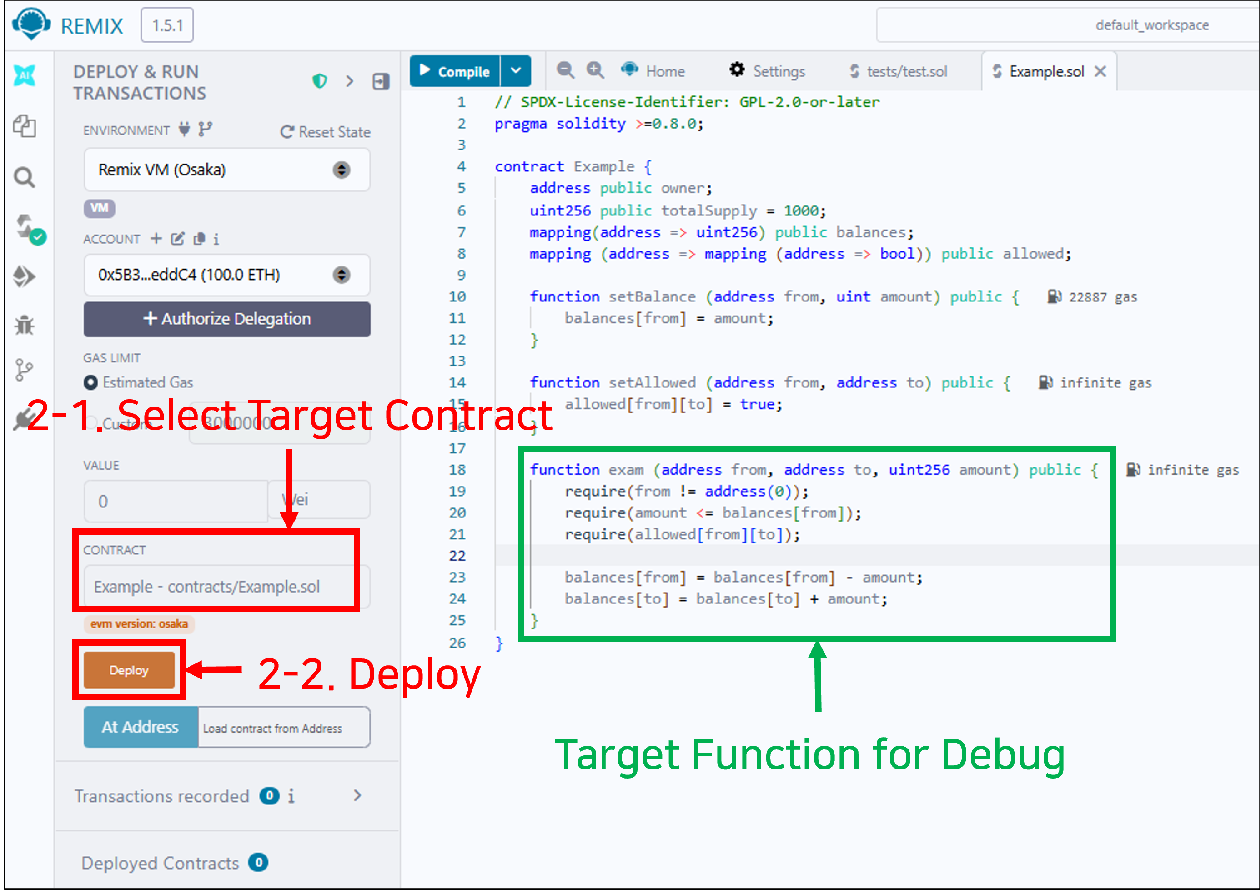
\includegraphics[width=0.9\columnwidth,height=0.35\textheight,keepaspectratio]{Fig2.pdf}
    \caption{Compilation in a conventional Solidity debugging workflow.}
    \label{fig:bg-compile}
\end{figure}
\FloatBarrier

\smallskip
\noindent\textbf{Step 2: Deploy.}
Before a contract can be executed, the compiled bytecode is deployed to a blockchain or a local blockchain environment.
As illustrated in Figure~\ref{fig:bg-deploy}, deployment creates a contract instance and invokes its constructor to initialize the contract state.
The deployed contract subsequently maintains persistent state across transactions.

\begin{figure}[!ht]
    \centering
    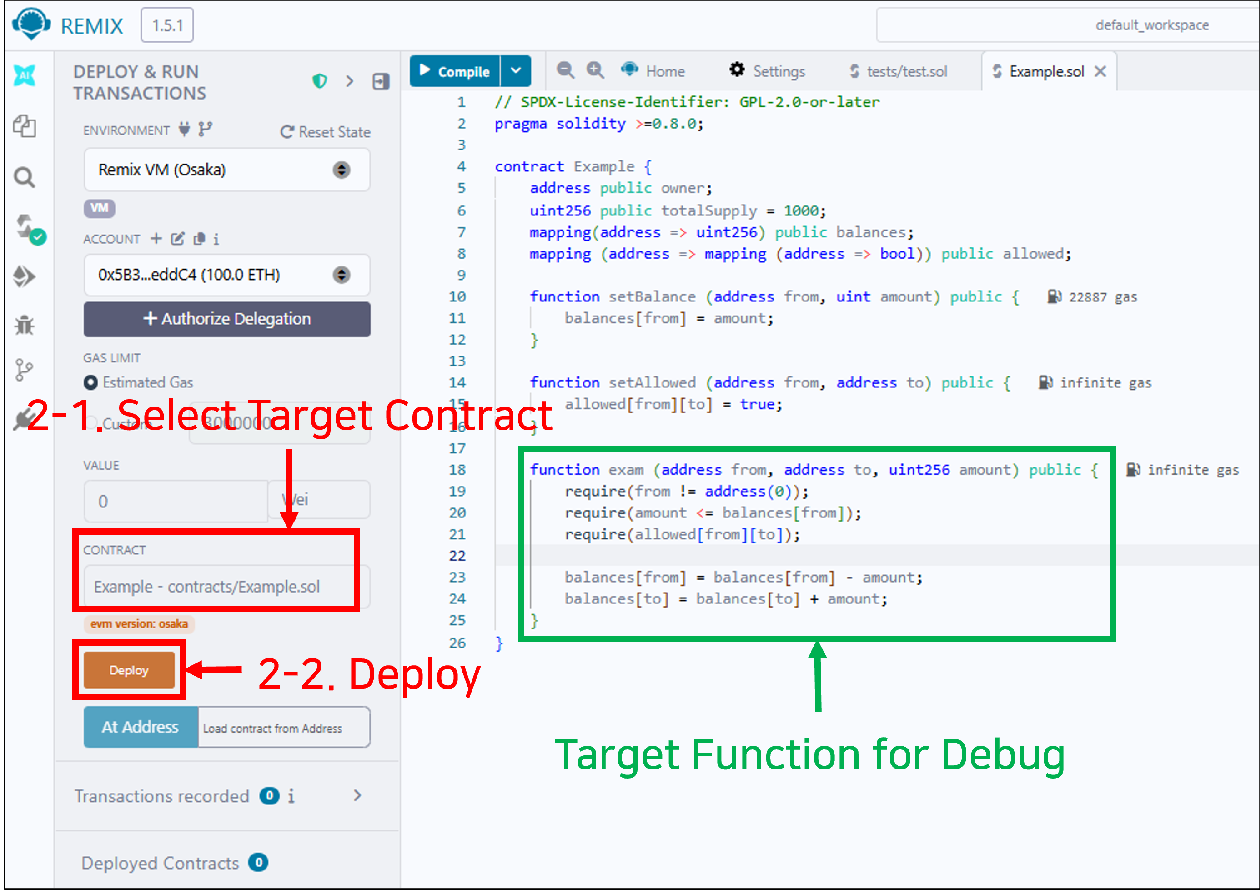
\includegraphics[width=0.9\columnwidth,height=0.3\textheight,keepaspectratio]{Fig3.pdf}
    \caption{Contract deployment in a conventional Solidity debugging workflow.}
    \label{fig:bg-deploy}
\end{figure}
\FloatBarrier

\smallskip
\noindent\textbf{Step 3: Initialize State and Execute.}
To inspect a target function, a developer must prepare an execution state in which the function can be invoked.
This preparation may require calling other functions in advance to initialize contract state or satisfy conditions enforced by constructs such as \texttt{require}.
Once the required state has been established, the developer supplies concrete function arguments and executes the target function as a transaction.
Figure~\ref{fig:bg-execute} shows an example of this process in Remix.

\begin{figure}[!ht]
    \centering
    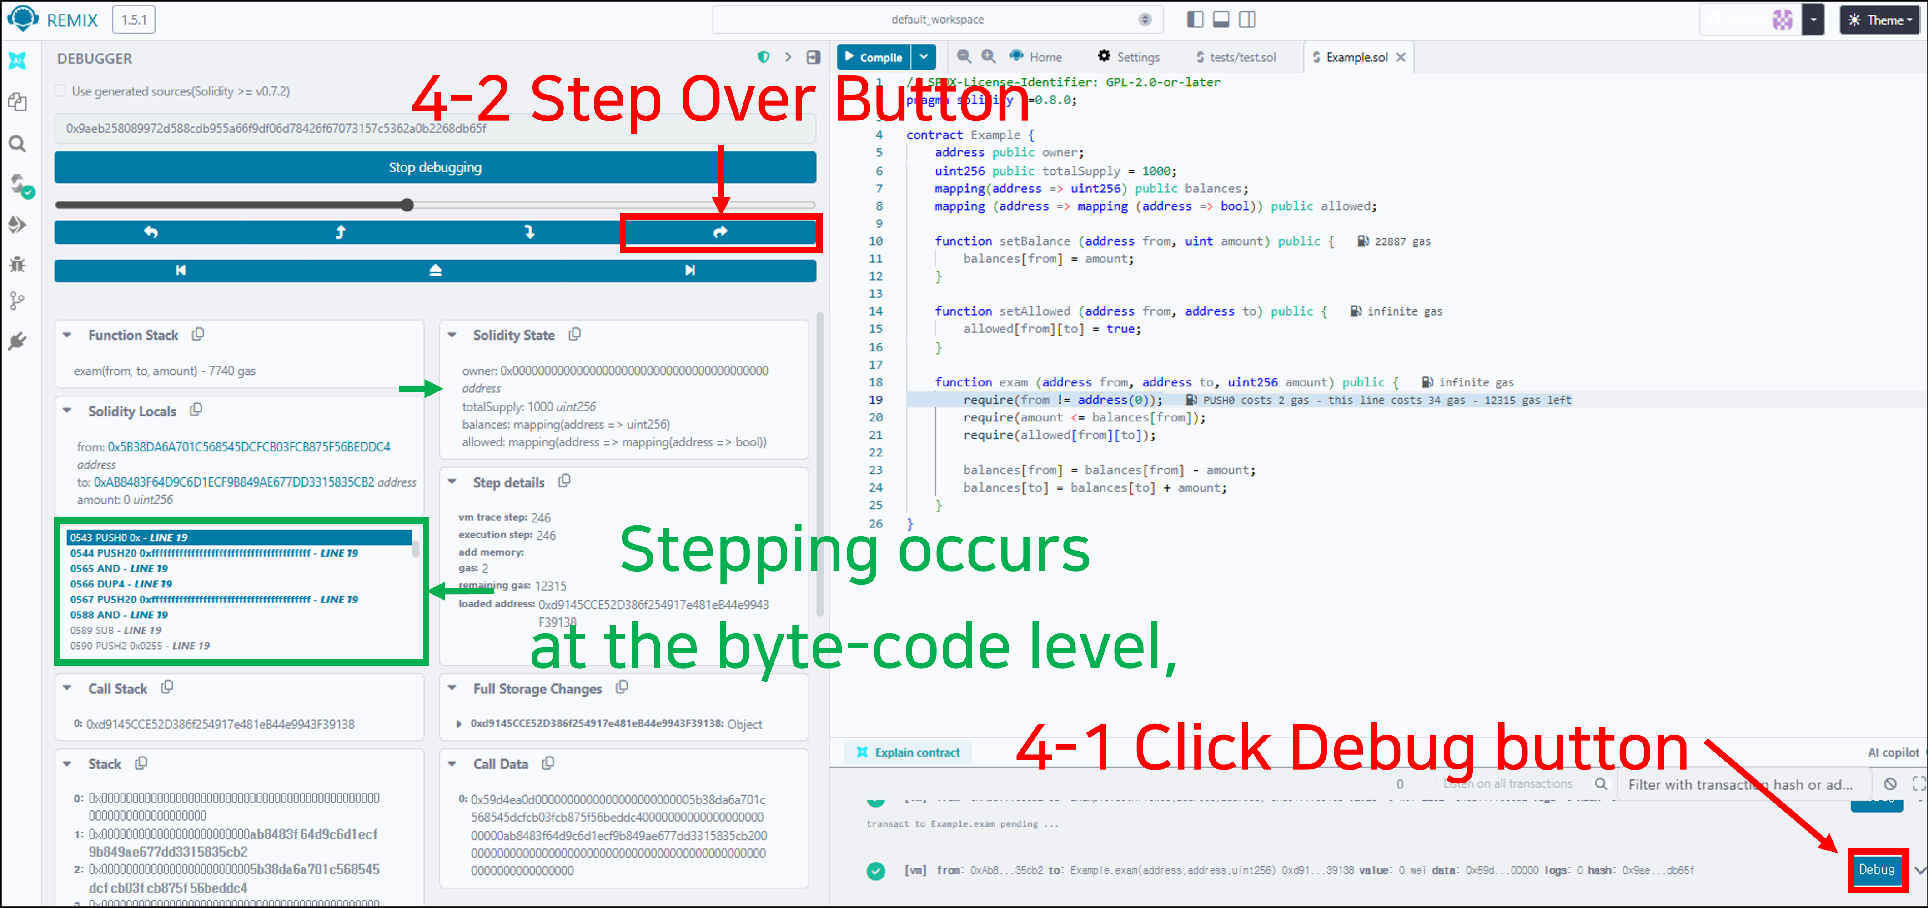
\includegraphics[width=0.9\columnwidth,keepaspectratio]{Fig4.pdf}
    \caption{State initialization and target-function execution in a conventional Solidity debugging workflow.}
    \label{fig:bg-execute}
\end{figure}
\FloatBarrier

\smallskip
\noindent\textbf{Step 4: Debug.}
After the target transaction has been executed, conventional Solidity debugging tools can expose its execution trace.
For example, Remix allows developers to inspect the executed transaction and step through the corresponding EVM instructions, as illustrated in Figure~\ref{fig:bg-debug}.
The debugger provides information such as the current opcode, stack and memory contents, storage values, and the relationship between bytecode instructions and source-code locations.

\begin{figure}[!ht]
    \centering
    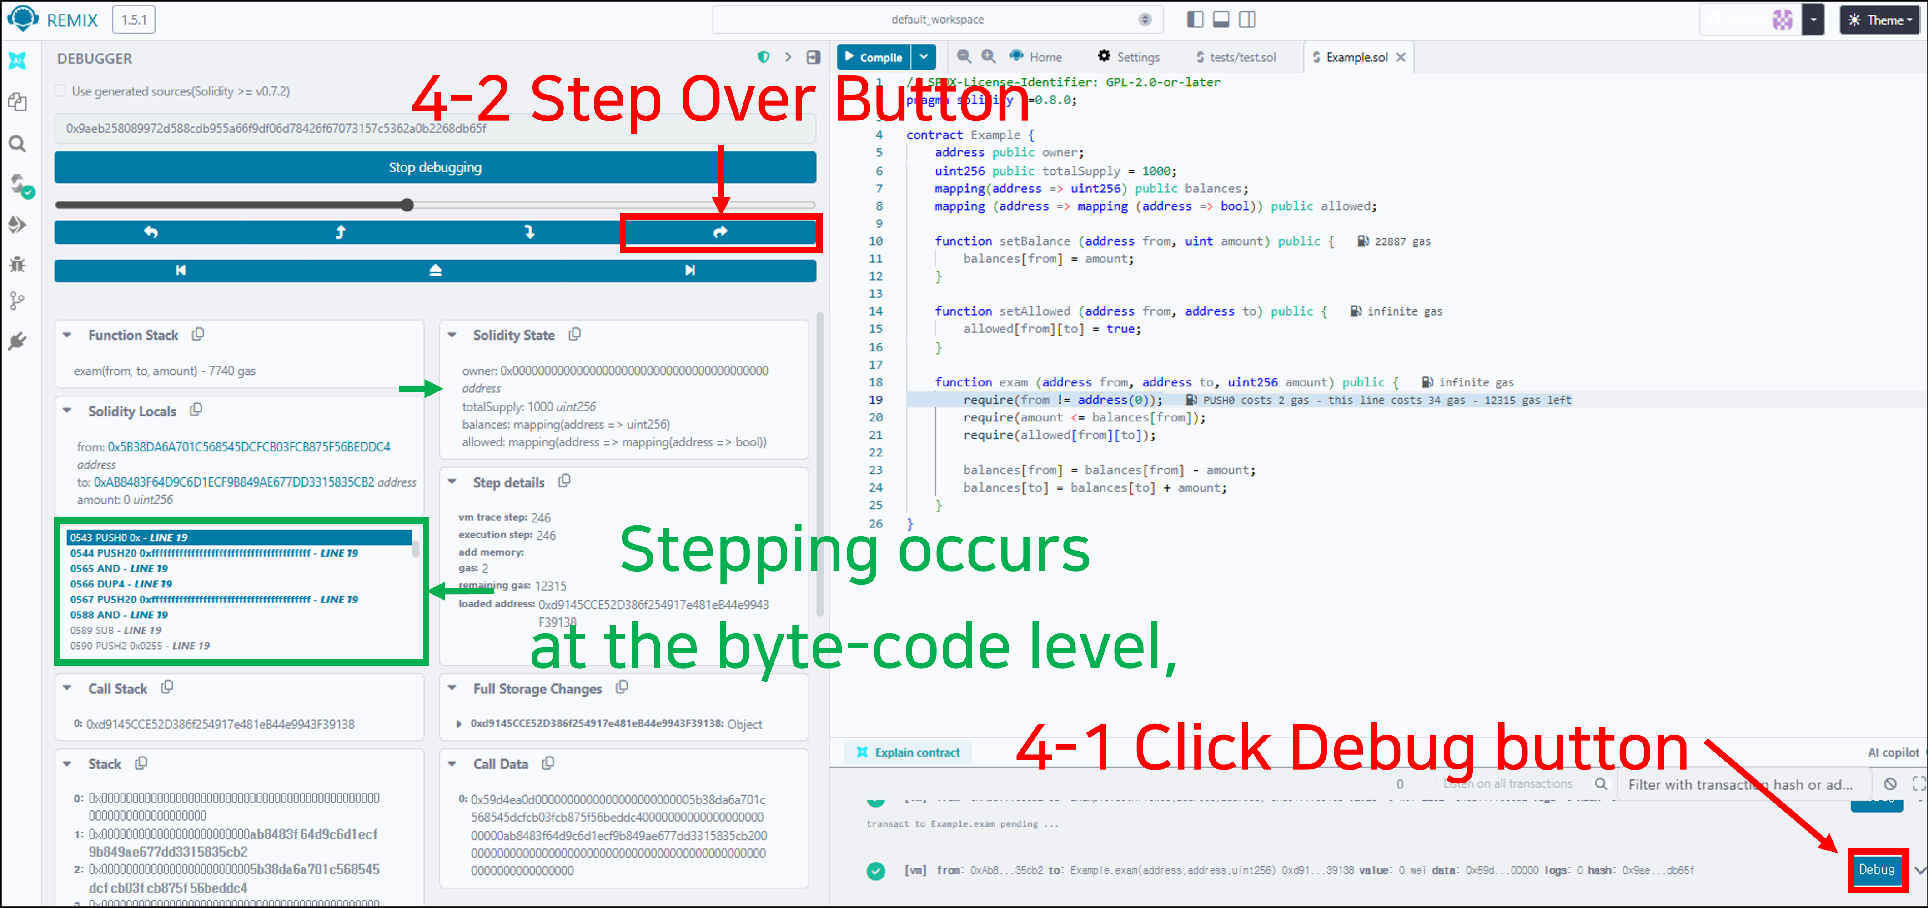
\includegraphics[width=1.0\columnwidth,keepaspectratio]{Fig5.pdf}
    \caption{Transaction-based bytecode debugging in a conventional Solidity debugging workflow.}
    \label{fig:bg-debug}
\end{figure}
\FloatBarrier

This workflow differs fundamentally from the edit--execute--debug cycle commonly available for traditional software.
In conventional Solidity debugging, the behavior to be inspected is materialized through a concrete execution: the contract is compiled and deployed, the required state is established, concrete inputs are supplied, and the resulting transaction trace is subsequently examined.
Accordingly, the observable debugging context is closely coupled to executable artifacts, initialized contract state, and a particular transaction execution.
These characteristics become particularly relevant when debugging support is considered during source-code development, where program behavior may need to be inspected before or while a complete concrete execution context is being prepared. 


%%%%%%%%%%%%%%%%%%%%%%%%%%%%%%%%%%%%%%%%%%%%%%%%%%%%%%%%%%%%%%%%%%%%%%%%%%%%%%%%
\section{Numeric Logic Errors in Solidity}\label{sec:bg:nle}
Recent studies have reported a variety of numeric-related weaknesses in smart contracts~\citep{numscout,gptscan,flyinointment,exploitablebugs,defiattacks}.
Unlike failures that trigger compilation errors, runtime exceptions, or transaction reverts, some numerical defects allow a transaction to complete successfully while producing values that are inconsistent with the intended behavior of the contract.
Following prior work, we refer to such defects as \textit{numeric logic errors}.

\begin{definition}[Numeric Logic Error]
A numeric logic error is a bug that allows a transaction to complete successfully without compile-time or runtime exceptions, but violates the developer's intended relationships among numerical values during function execution.
\end{definition}

This definition emphasizes an important characteristic of numeric logic errors.
Whether a numerical computation is erroneous cannot always be determined solely from the fact that execution succeeds or from the syntactic form of the computation.
Instead, correctness depends on whether the resulting numerical relationships conform to the behavior intended by the developer.
For example, two arithmetic expressions may both be syntactically valid and execute without reverting, while only one preserves the intended relationship among balances, exchange amounts, rewards, or accounting variables.
Thus, the intended numerical relationship constitutes part of the criterion by which such program behavior is judged.

Numeric logic errors can be distinguished according to the execution scope in which they manifest.
\textit{Single-transaction errors} arise within one atomic transaction.
The relevant computations may span multiple internal or external function calls, but the behavior leading to the erroneous numerical result is contained within a single transaction.
In contrast, \textit{multiple-transaction errors} emerge only through a sequence of transactions and therefore depend on state changes accumulated across multiple function invocations.
Examples include Risky First Deposit and Price Oracle Manipulation~\citep{gptscan,exploitablebugs}, whose effects become observable only after contract state has evolved over multiple transactions.

This dissertation primarily focuses on single-transaction numeric logic errors, including cases in which a transaction crosses contract boundaries through external calls.
This scope is consistent with the development-time analysis considered throughout the dissertation: the behavior of interest is bounded by one transaction and can therefore be analyzed with respect to the source-level execution being examined.
Numeric properties that inherently span arbitrary transaction sequences require reasoning about inter-transaction dependencies and contract-level invariants and are left outside the primary scope of this work.

Within the single-transaction scope, representative numeric logic errors can be organized according to the abstraction level at which the erroneous behavior arises.
Table~\ref{tab:nle-patterns} summarizes representative patterns reported in prior studies.

\begin{table}[t]
\centering
\caption{Representative single-transaction numeric logic error patterns from prior work, classified by abstraction level.}
\label{tab:nle-patterns}
\footnotesize
% Relative widths, not cm: the B5 measure is 116 mm (330.05 pt), so the
% 4.2 cm + 8.5 cm this table originally used overran the right margin by 15 mm
% -- silently, because \centering inside a float suppresses the Overfull report.
\begin{tabular}{@{}p{0.29\textwidth}p{0.67\textwidth}@{}}
\toprule
Pattern & Description \\
\midrule

\multicolumn{2}{@{}p{\dimexpr0.96\textwidth+2\tabcolsep\relax}@{}}{\textit{\textbf{Value-level errors: incorrect numerical values arise directly from computations.}}} \\
\midrule

Div In Path~\citep{numscout}
& Division results used in conditions may alter control-flow decisions because of integer truncation. \\

Exchange Problem~\citep{numscout}
& Rounding behavior in exchange calculations may produce an unintended output, such as zero output for a valid input or an imbalanced exchange. \\

Precision Loss Trend~\citep{numscout}
& Repeated or improperly ordered integer arithmetic may systematically introduce truncation that favors one side of a computation. \\

Minor Amount Retention~\citep{numscout}
& Integer division in distribution logic may leave numerical remainders unallocated. \\

\midrule
\multicolumn{2}{@{}p{\dimexpr0.96\textwidth+2\tabcolsep\relax}@{}}{\textit{\textbf{Algorithm-level errors: incorrect numerical behavior arises from the structural arrangement of operations.}}} \\
\midrule

Operator Order Issue~\citep{numscout}
& Different arithmetic evaluation orders can produce different integer results because intermediate truncation is not preserved across algebraically equivalent expressions. \\

Erroneous Accounting / Wrong Interest Rate Order~\citep{gptscan,exploitablebugs}
& Balance calculations use stale or prematurely updated interest-rate information, resulting in an incorrect numerical outcome. \\

Erroneous Accounting / Wrong Checkpoint Order~\citep{gptscan,exploitablebugs}
& State updates and checkpoints are performed in an incorrect order, causing subsequent reward or accounting calculations to use unintended values. \\

Inconsistent State Updates~\citep{exploitablebugs}
& A required state update is omitted, leaving subsequent computations to operate on stale numerical state. \\

Greedy Contract~\citep{flyinointment}
& The contract accepts funds but lacks the corresponding operation needed to release them, resulting in an unintended numerical state. \\

\bottomrule
\end{tabular}
\end{table}

\textbf{Value-level errors} arise when the computation directly produces an unintended numerical value.
Typical examples include the use of an incorrect operator or identifier, precision loss caused by integer arithmetic, or an arithmetic expression whose result differs from the value intended by the developer.
The erroneous behavior is therefore observable primarily through the values produced by the computation.

\textbf{Algorithm-level errors}, in contrast, arise from the structural arrangement of operations.
Examples include executing otherwise valid operations in an incorrect order, omitting a required state update, or failing to perform a necessary procedure call.
Although their underlying cause is structural, their effect may still become observable as an unintended relationship among numerical values.

The distinction between value-level and algorithm-level errors provides an organizing basis for characterizing the numeric logic errors considered in this dissertation.
The next chapter reviews related work on Solidity debugging and analysis, including existing approaches to numeric logic error detection.


%%%%%%%%%%%%%%%%%%%%%%%%%%%%%%%%%%%%%%%%%%%%%%%%%%%%%%%%%%%%%%%%%%%%%%%%%%%%%%%%
\chapter{Related Work}\label{chap:related}

\section{Solidity Debugging and Development Environments}
\label{sec:rel:debugging}
Modern Solidity development environments either embed a debugger or integrate external debugging plug-ins. 
Remix IDE~\citep{remix} is a widely used web-based development environment that provides Solidity editing, compilation, deployment, and transaction debugging. Its debugger operates over executed transactions and allows developers to inspect EVM-level information such as instructions, stack, memory, and storage.
Hardhat~\citep{hardhat} is a Node.js-based development framework that provides Solidity compilation, local blockchain execution, testing, and deployment support. Visual Studio Code extensions can integrate with Hardhat to provide step-by-step debugging of transaction executions. 
Forge~\citep{forge}, part of the Foundry toolchain, focuses on fast and reproducible testing. It executes Solidity tests on a local EVM and supports debugging of concrete test executions through Forge Debug. 
Solidity Debugger Pro~\citep{soldepro} is a Visual Studio Code extension that similarly supports runtime debugging over concrete transactions in conjunction with Hardhat.

These environments provide practical support for inspecting concrete smart-contract executions, but their debugging workflows are generally tied to compiled artifacts, deployed or locally instantiated contract state, and executed transactions. In contrast, the approach presented in this dissertation focuses on inspecting program behavior directly at the Solidity source-code level without requiring a separate concrete transaction execution for each debugging scenario.

\section{Numeric Logic Error Detection in Solidity}
\label{sec:rel:nle}
Several studies have proposed techniques for detecting numeric and logic-related errors in Solidity smart contracts.
These approaches differ in the types of numerical defects they target and in the criteria used to identify erroneous behavior.

NumScout~\citep{numscout} focuses specifically on numerical defects in smart contracts.
It defines five defect patterns---Div In Path, Operator Order Issue, Exchange Problem, Precision Loss Trend, and Minor Amount Retention---and detects their occurrences using symbolic execution guided by an LLM-based pruning mechanism.
Its detection criteria are therefore derived from predefined numerical defect patterns.
GPTScan~\citep{gptscan} targets a broader set of logic vulnerabilities, including accounting-related errors.
It combines GPT-based scenario matching with lightweight static analysis~\citep{slither} to identify code that conforms to predefined vulnerability scenarios.
Among its supported cases are numerical logic errors involving incorrect accounting operations, update ordering, and related financial computations.
ScType~\citep{sctype} approaches numerical correctness from a type-based perspective.
It extends Solidity variables with financial type information represented as tuples of $\langle$financial type, scaling factor, token unit, address$\rangle$ and detects inconsistent financial operations through type checking.
Unlike pattern-based detectors, ScType can incorporate developer-provided type annotations when the required financial information cannot be inferred directly from the source code.

Other studies address broader forms of logic errors beyond single-transaction numerical behavior.
For example, SmartInv~\citep{smartinv} infers invariants from source code and natural-language artifacts to detect machine-unauditable bugs, while several approaches analyze multi-transaction behaviors such as price manipulation~\citep{defiranger,defiguard,pomabuster,secplf,defitainter} and flash-loan attacks~\citep{defitail,midnight}.
These approaches extend logic-error detection to properties that depend on inferred invariants or state changes across multiple transactions.

Overall, existing numeric logic error detectors primarily identify erroneous behavior through predefined defect patterns, vulnerability scenarios, or domain-specific consistency rules.
They provide automated detection for the classes of errors represented by their respective analysis models.
The approach presented in this dissertation instead focuses on validating numerical relationships explicitly supplied by developers during development.

\section{Specification-Based Smart Contract Analysis}
\label{sec:rel:intent}
Specification-based smart contract analysis allows developers to explicitly state expected program properties and check whether contract implementations satisfy them using testing, symbolic execution, or formal verification backends.

Scribble~\citep{scribble} translates developer-written specifications into Solidity assertion code so that the resulting properties can be checked using existing analysis and testing tools such as MythX~\citep{mythx} and Mythril~\citep{mythril}.
It supports several forms of specification, including \texttt{if\_succeed} for conditions on successful function completion, invariant for contract-level properties, \texttt{if\_updated} for conditions associated with state updates, and \texttt{assert} for properties at specific execution points.
SmartACE~\citep{smartace} builds on Scribble specifications and verifies Solidity contracts through LLVM-IR-based verification harnesses using tools such as SeaHorn~\citep{seahorn}, libFuzzer~\citep{libfuzzer}, and KLEE~\citep{klee}.
It also abstracts the Ethereum address space into a finite set of representative users to reason about properties involving multiple participants and aggregate accounting behavior.
Idealist~\citep{idealist} distinguishes between annotations that provide assumptions for verification, such as loop invariants, call invariants, and call modifies, and annotations that express verification obligations, including \texttt{ensures}, \texttt{reverts\_if}, and contract invariants.
These annotations support reasoning about function postconditions, revert behavior, and contract-level invariants.
Solvent~\citep{solvent} focuses on user-specified liquidity properties.
It translates both the contract and the supplied properties into SMT constraints and checks their satisfiability, producing counterexamples when a property can be violated.

These approaches demonstrate the value of explicit developer-supplied specifications for checking smart-contract behavior.
They generally target broad contract properties and rely on verification, symbolic reasoning, or instrumented assertion checking to determine whether those properties hold.
In contrast, the approach presented in this dissertation focuses specifically on developer-authored numerical relationships associated with source-level program states and evaluates them over abstract program states during debugging.

\section{Abstract Interpretation and Interactive Static Analysis}
\label{sec:rel:ai}
Interactive and incremental abstract interpretation has been actively studied for traditional programming languages.
Several studies have integrated incremental or demand-driven analysis into development environments for languages such as C and Java, providing analysis results while programs are being edited~\citep{daig,ds,iac,iaj,fap}.

\citet{daig} proposed demanded abstract interpretation, which incrementally reconstructs only the analysis components affected by program changes.
A subsequent study by \citet{ds} extended this approach to procedure summaries, enabling inter-procedural analysis results to be reused across edits.
\citet{iac} introduced incremental analysis support for Goblint, selectively recomputing affected analysis facts for multithreaded C programs.
For Java, \citet{iaj} presented IntraJ, an analyzer integrated through the Language Server Protocol that computes only the syntax and data-flow information required for the current development context.
\citet{fap} proposed an efficient interval-analysis technique over call graphs and later extended it with incremental analysis that revisits only functions affected by program modifications.

These studies demonstrate the feasibility of interactive and incremental abstract interpretation for providing responsive analysis during development.
In contrast, IQDebug uses program-point abstract states as a source-level debugging context for Solidity and evaluates developer-authored numerical intent over these states.

\chapter{The Design of IQDebug}\label{chap:design}
\section{System Architecture}\label{sec:design:overview}

Figure~\ref{fig:design:architecture} illustrates the overall architecture of IQDebug.
The system processes its inputs through three phases: source processing, analysis, and intent validation.

\smallskip
\noindent\textbf{Input.}
IQDebug receives four types of input:

\begin{itemize}
    \item \textbf{Solidity source fragments} represent statements or code fragments to be incorporated into the currently analyzed program.
    \item \textbf{Debugging inputs} specify values used to establish a debugging scenario.
    \item \textbf{Developer intent} describes numerical relationships to be validated over the analyzed program states.
    \item \textbf{Dependency CFGs} provide precomputed control-flow information for referenced contracts when cross-contract analysis is required.
\end{itemize}

\begin{figure}[!t]
    \centering
    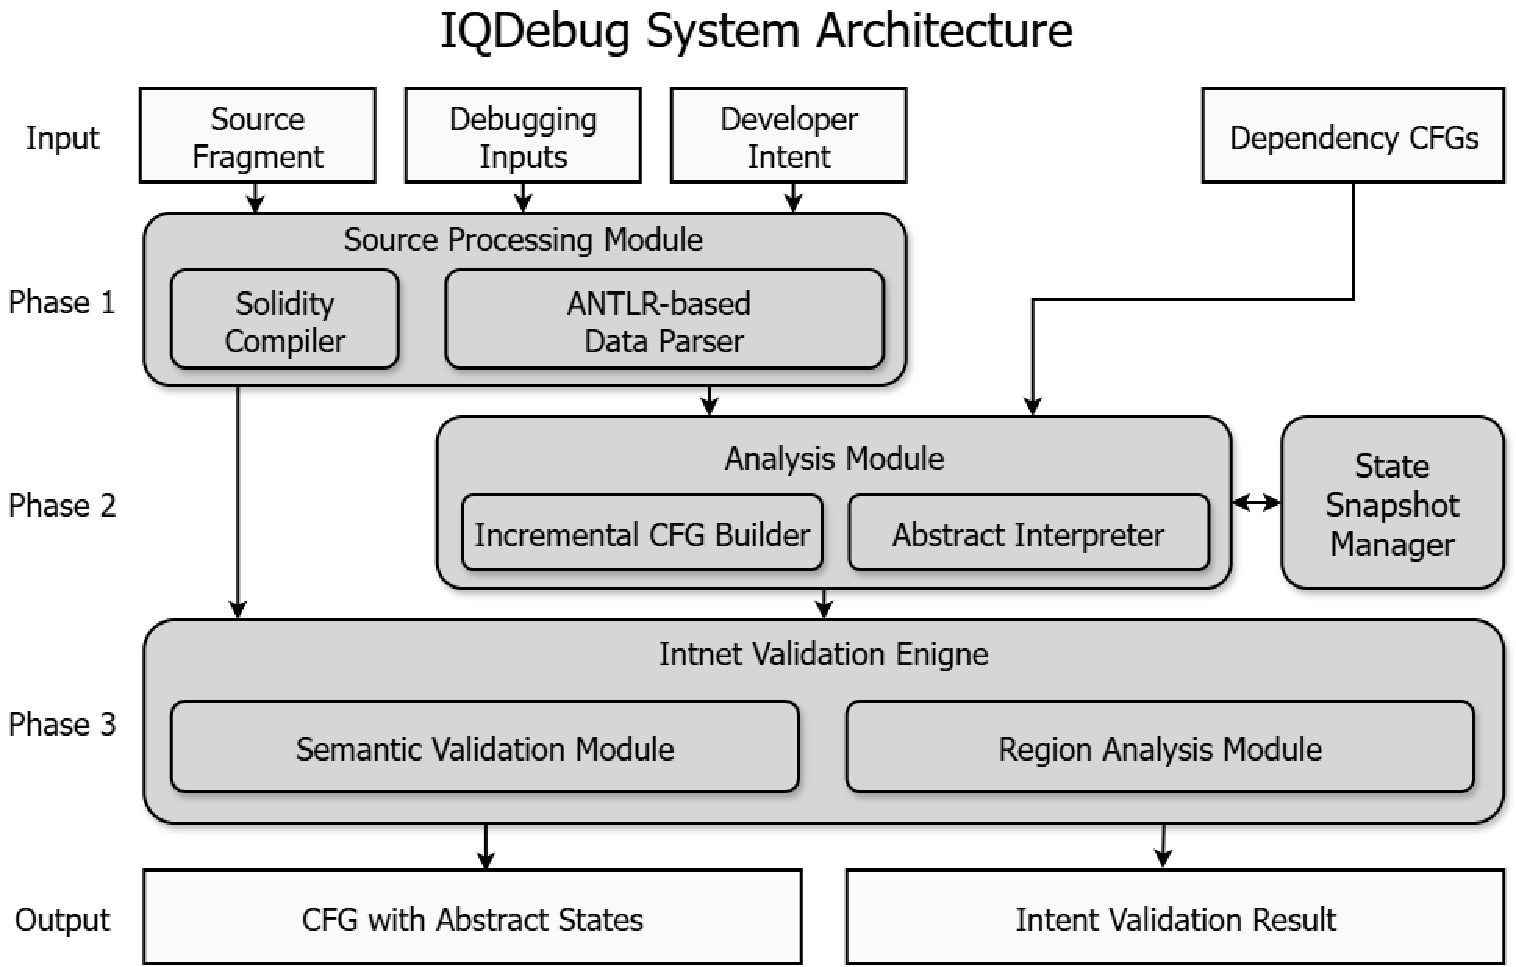
\includegraphics[width=\columnwidth,keepaspectratio]{Fig6.pdf}
    \caption{Overall architecture of \tool{}.}
    \label{fig:design:architecture}
\end{figure}

\smallskip
\noindent\textbf{Phase 1: Source Processing.}
The Source Processing Module receives the source fragment, debugging inputs, and developer intent.
The Solidity compiler checks whether the incoming source fragment can be inserted into the existing contract source without introducing syntactic errors.
The ANTLR-based data parser processes the source fragment, debugging inputs, and developer intent according to the extended Solidity grammar.
The parsed source and debugging information is forwarded to the Analysis Module, while the parsed intent information is provided to the Intent Validation Engine.

\smallskip
\noindent\textbf{Phase 2: Analysis.}
The Analysis Module incrementally updates the source-level control-flow graph and computes abstract program states.
The Incremental CFG Builder determines where a newly processed source statement should be inserted into the existing CFG, while the Abstract Interpreter evaluates the statement and propagates its effects to affected downstream program points.
When external contract behavior is required, precomputed dependency CFGs are supplied to the Analysis Module to support cross-contract analysis.
Inherited contract code and referenced libraries are analyzed within the target contract's execution context, while calls to separately deployed external contracts are analyzed only when the corresponding dependency CFG is available.
If such a dependency CFG is unavailable, the callee's internal state transitions are not incorporated into the analysis, and values returned from the call may remain unknown unless they are explicitly supplied as debugging inputs.
The State Snapshot Manager preserves the analysis state before debugging inputs are applied.
After the debugging inputs are interpreted and the corresponding abstract states are computed, the preserved state can be restored so that separate debugging scenarios do not permanently modify the underlying analysis context.
The resulting CFG stores the computed abstract states at its program points and serves as the primary representation used for source-level debugging.

\smallskip
\noindent\textbf{Phase 3: Intent Validation.}
The Intent Validation Engine evaluates developer intent against the abstract states produced by the Analysis Module.
The Semantic Validation Module determines whether the analyzed behavior satisfies, violates, or cannot conclusively establish the specified numerical relationship.
The Region Analysis Module further analyzes relevant abstract value regions to provide diagnostic information associated with the validation result.

\smallskip
\noindent\textbf{Output.}
IQDebug produces two main outputs:

\begin{itemize}
    \item \textbf{CFG with abstract states} is a source-level control-flow graph in which abstract program states are stored at individual program points.
    \item \textbf{Intent validation result} reports the outcome of evaluating developer intent against the corresponding abstract program states.
\end{itemize}

These outputs are used by the debugging interface to inspect program behavior directly at the Solidity source-code level.
Because abstract states are computed in advance and stored at source-level program points in the CFG, the debugger can reuse these stored results as long as the source code and debugging inputs remain unchanged.
Under this condition, stepping or moving between breakpoints only requires reading the stored states rather than re-running the Abstract Interpreter at every navigation step.

\section{Source-Level Program Analysis}\label{sec:design:analysis}
IQDebug analyzes Solidity programs directly at the source-code level.
The analysis maintains a source-level control-flow graph that evolves as source fragments are added or modified, and computes abstract program states over this representation.
This section first describes how Solidity source code is represented and incrementally incorporated into the CFG, then presents the debugging input model and the abstract interpretation used to compute program states.

\subsection{Source-Level Program Representation}\label{subsec:design:representation}
IQDebug maintains a source-level representation of a Solidity program that evolves with source-code edits.
Rather than requiring a complete program to be processed at once, IQDebug incrementally incorporates individual source fragments into the existing representation.
This process consists of parsing incoming source fragments, representing their control-flow semantics in the source-level CFG, maintaining mappings between source locations and CFG nodes, and updating the representation as the source code is inserted, deleted, or modified.

\subsubsection{Source fragments and interactive parsing}
\label{subsubsec:design:representation:parsing}
IQDebug processes Solidity source code at the granularity of source fragments.
The accepted fragments are divided into two types:

\begin{itemize}
  \item \textbf{Block fragment:} Includes contract and function definitions and control-flow constructs such as \texttt{if}/\texttt{else} blocks and loops. When the developer types an opening \texttt{\{}, most editors automatically insert the corresponding closing \texttt{\}}, allowing the structural block to be processed before its body is fully populated.

  \item \textbf{Statement fragment:} Includes declarations, assignments, function calls, and other expressions that terminate with a semicolon. Each statement can be processed individually when it is completed by the developer.       
\end{itemize}

A source fragment does not necessarily constitute a complete Solidity program by itself.
IQDebug therefore uses an ANTLR-based parser with an extended Solidity grammar that provides specialized entry rules for incremental source processing.
These rules allow individual fragments to be parsed according to both their syntactic form and their relationship with the source code that has already been processed.
Table~\ref{tab:interactive-rules} summarizes the seven entry rules for Solidity source constructs.

\begin{table}[!t]
\centering
\caption{Interactive parser entry rules}
\label{tab:interactive-rules}
\small
% p{8cm} overran the 116 mm measure by 27.4 pt: the "Entry Rule" column does not
% wrap (interactiveCatchClauseUnit is ~46 mm on its own), so the Purpose column
% has to be narrower here than it would be in a two-column paper.
\begin{tabular}{@{}c|lp{6.7cm}@{}}
\toprule
\textbf{Type} & \textbf{Entry Rule} & \textbf{Purpose} \\
\midrule
\multirow{2}{*}[-10pt]{Primary} & interactiveSourceUnit & Top-level declarations: functions, contracts, interfaces, libraries, state variables, pragmas, imports \\
& interactiveBlockUnit & Statements and control-flow skeletons inside function bodies \\
\midrule
\multirow{5}{*}[-8pt]{Continuation} & interactiveEnumUnit & Enum member items added after the enum shell is defined \\
& interactiveStructUnit & Struct member declarations added after the struct shell is defined \\
& interactiveDoWhileUnit & The while tail of a do-while loop \\
& interactiveIfElseUnit & else or else-if branches following an if statement \\
& interactiveCatchClauseUnit & catch clauses following a try statement \\
\bottomrule
\end{tabular}
\end{table}

As shown in Table~\ref{tab:interactive-rules}, the entry rules are divided into \textit{primary} and \textit{continuation} rules.

\begin{itemize}
  \item \textbf{Primary rules} handle constructs that can be parsed without depending on a preceding source construct.

  \item \textbf{Continuation rules} handle fragments whose syntactic role depends on an already existing construct. For example, \texttt{interactiveIfElseUnit} requires a preceding \texttt{if} or \texttt{else if} statement to determine where an incoming \texttt{else} branch belongs.
\end{itemize}

IQDebug also verifies that each source edit preserves the syntactic validity of the complete Solidity program.
The incoming fragment is incorporated into the currently maintained source code to construct a candidate program, which is then checked by the Solidity compiler.
If the resulting program is syntactically invalid, the edit is rejected before the source-level CFG is updated.
Otherwise, the parsed source construct is forwarded to the Incremental CFG Builder, which incorporates its control-flow structure into the existing CFG.

\subsubsection{Source-Level CFG Representation}
\label{subsubsec:design:representation:cfg}
IQDebug represents Solidity programs using a hierarchical source-level CFG.
The CFG serves as the common representation for incremental source processing, abstract interpretation, and subsequent source-level debugging.
Each node corresponds to a source-level program point, allowing abstract program states and intent-validation results to be associated with positions in the Solidity source code.

\noindent\textbf{CFG hierarchy.}
IQDebug organizes the CFG at two levels.
At the contract level, a \texttt{ContractCFG} represents state-variable initialization, constructor execution, and the functions defined in the contract (Figure~\ref{fig:contract-cfg}).
State variables are initialized before the constructor, and the constructor may subsequently update the initialized state.
Each function is represented by a separate \texttt{FunctionCFG} that models control flow from function entry to its possible termination points (Figure~\ref{fig:function-cfg}).
When a function declares modifiers, the modifier control flow surrounds the function body, with the modifier placeholder (\texttt{\_}) marking the position at which the function body is inserted.
For function calls, the corresponding callee CFG is connected to the caller's control-flow context.
If the callee belongs to an external contract whose dependency CFG is available, IQDebug uses the supplied dependency CFG to represent the called function.

\smallskip
\noindent\textbf{CFG node types.}
Both \texttt{ContractCFG} and \texttt{FunctionCFG} are composed of source-level CFG nodes that represent different control-flow roles.
IQDebug uses the following node types:

\begin{itemize}
  \item \texttt{entry node}: Represents the unique entry point of a contract-level or function-level CFG.

  \item \texttt{state variable node}: Represents contract state-variable declarations. State-variable declarations are grouped into a contract-level node because they do not introduce control-flow branches.

  \item \texttt{basic node}: Represents a source-level statement with sequential control flow, including variable declarations, assignments, function calls, \texttt{return}, and \texttt{revert} statements.

  \item \texttt{condition node}: Represents constructs that divide control flow according to a condition, including \texttt{if}, \texttt{else if}, loops, \texttt{require}/\texttt{assert}, and \texttt{try} constructs.

  \item \texttt{join node}: Represents a program point at which control flows from alternative branches are merged.

  \item \texttt{fixpoint evaluation node} (\(\phi\)): Represents the merge point for successive loop iterations and is used for fixpoint computation during abstract interpretation.

  \item \texttt{loop exit node}: Represents the control-flow point reached when execution leaves a loop through its false condition or a corresponding loop-exit path.

  \item \texttt{return exit node}: Represents the common destination of return paths within a function.

  \item \texttt{error exit node}: Represents exceptional termination caused by constructs such as \texttt{revert} or failed \texttt{require}/\texttt{assert} conditions.

  \item \texttt{exit node}: Represents the unique normal exit point of a contract-level or function-level CFG.
\end{itemize}

\noindent\textbf{Statement-local CFG construction.}
Within a \texttt{FunctionCFG}, each Solidity statement is translated into a CFG structure according to its control-flow semantics.
This statement-local representation defines how sequential execution, branching, loops, and abrupt control-flow changes are represented before incremental source updates are applied.

\begin{itemize}

  \item \textbf{Simple statements} create a single \texttt{basic node} between the preceding and succeeding control-flow points. This category includes variable declarations, assignments, and function calls (Figure~\ref{fig:new-simple-statement}).

  \item \textbf{If statements} create a \texttt{condition node}, true and false branches, and an \texttt{if join} at which the branch flows are merged (Figure~\ref{fig:new-if}).

  \item \textbf{Else-if clauses} extend the false branch of the preceding conditional with an additional \texttt{condition node} and branch structure before reconnecting to the outer join (Figure~\ref{fig:new-else-if}).

  \item \textbf{Else clauses} replace the remaining false branch with an explicit alternative branch that reconnects to the corresponding join node (Figure~\ref{fig:new-else}).

  \item \textbf{Loops} create a \texttt{fixpoint evaluation node} (\(\phi\)), a loop-condition node, a loop-body path, and a \texttt{loop exit node}. The body reconnects to the fixpoint node so that repeated iterations can be summarized during abstract interpretation (Figure~\ref{fig:new-while}).

  \item \textbf{Break statements} redirect control flow to the corresponding \texttt{loop exit node} (Figure~\ref{fig:new-break}), whereas \textbf{continue statements} redirect control flow to the loop's \(\phi\) node (Figure~\ref{fig:new-continue}).

  \item \textbf{Return statements} redirect control flow to the function's unique \texttt{return exit node} (Figure~\ref{fig:new-return}).

  \item \textbf{Require/assert statements} are represented by a \texttt{condition node}. The successful branch continues normal execution, while the failing branch leads to the \texttt{error exit node} (Figure~\ref{fig:new-require}).

  \item \textbf{Revert statements} terminate the current execution path by connecting directly to the \texttt{error exit node} (Figure~\ref{fig:new-revert}).

\end{itemize}

\begin{table}[t!]
\centering
\caption{Line-to-node index mapping by statement type}
\label{tab:line-mapping}
\small
\begin{tabular}{@{}lll@{}}
\toprule
\textbf{Statement} & \textbf{Maps Start Line To} & \textbf{Maps End Line To} \\
\midrule
\multicolumn{3}{@{}l}{\textit{\textbf{Simple statements}}} \\
\texttt{simple statement} & basic node & (none) \\
\texttt{break} & basic node & (none) \\
\texttt{continue} & basic node & (none) \\
\texttt{return} & basic node & (none) \\
\texttt{revert} & basic node & (none) \\
\texttt{require/assert} & condition node & (none) \\
\midrule
\multicolumn{3}{@{}l}{\textit{\textbf{Compound statements}}} \\
\texttt{if} & condition node & join node \\
\texttt{else if} & condition node & join node \\
\texttt{else} & basic node & join node \\
\texttt{while} & condition node & loop exit node \\
\bottomrule
\end{tabular}
\end{table}

\subsubsection{Line-to-Node Mapping}
\label{subsubsec:design:representation:mapping}
The statement-local CFG structures described above define how individual Solidity constructs are represented in the control-flow graph.
For incremental source processing, however, IQDebug must additionally maintain a correspondence between source-code locations and the CFG nodes representing those locations.
This correspondence is required because a newly inserted source fragment is identified by its position in the source code, whereas the CFG itself represents control-flow relationships rather than textual positions.
IQDebug therefore maintains a line-to-node index \(M\) that associates source lines with the corresponding CFG nodes.
The mapping reflects the CFG structure created for each statement type, as summarized in Table~\ref{tab:line-mapping}. 

Simple statements require only a mapping from their source line to the node that directly represents the statement.
Most simple statements therefore map to a \texttt{basic node}, whereas \texttt{require} and \texttt{assert} map to a \texttt{condition node} because their successful and failing outcomes form separate control-flow paths.

Compound constructs additionally require their structural boundaries to be represented.
For \texttt{if} and \texttt{else if} statements, the start line maps to the corresponding \texttt{condition node}, while the end line maps to the \texttt{join node} at which their branch flows converge.
An \texttt{else} block maps its start line to the entry of the alternative branch and its end line to the corresponding join node.
Similarly, a loop maps its start line to the loop condition and its end line to the \texttt{loop exit node}.

The line-to-node mapping provides the bridge between textual source edits and their corresponding positions in the CFG. IQDebug uses this mapping to locate insertion points, identify deletion boundaries, and determine the nodes affected by source modifications.

\subsubsection{Incremental Source-Code Updates}
\label{subsubsec:design:representation:updates}
IQDebug supports three types of incremental source-code updates: insertion, deletion, and modification.
Each update modifies the existing source-level CFG in place rather than reconstructing the entire graph.
After an update, abstract interpretation is resumed from the affected program point so that changes are propagated to downstream states while unaffected analysis results can be reused.

\smallskip
\noindent\textbf{Code insertion.}
When a new source fragment is inserted, IQDebug first determines the CFG position at which the corresponding control-flow structure should be attached.
The lookup procedure differs depending on whether the incoming fragment requires a previously established control-flow context.

\begin{algorithm}[!t]
\caption{Dependent-Context Lookup}
\label{alg:get-branch-context}
\begin{algorithmic}[1]
\State \textbf{Input:} CFG $G$, line-to-node index $M$, current line $L$
\State \textbf{Output:} Condition node $c$
\Function{GetBranchContext}{$G, M, L$}
\State $queue \gets \texttt{FindJoinNode}(M, L)$
\Comment{find join node at or before line $L$}

\If{$queue=\emptyset$}
\State \textbf{error} ``No join node found at or before line $L$''
\EndIf

\State $visited \gets \emptyset$

\While{$queue\neq\emptyset$}
\State $n \gets \texttt{Dequeue}(queue)$

\If{$n\in visited$}
  \State \textbf{continue}
\EndIf

\State $visited \gets visited\cup\{n\}$

\If{$\texttt{IsCond}(G,n)$ \textbf{and}
    $\texttt{CondType}(n)\in\{\texttt{if},\texttt{else\_if}\}$}
  \State \Return $n$
\EndIf

\For{$p\in\texttt{Pred}(G,n)$}
  \If{$p\notin visited$}
    \State $\texttt{Enqueue}(queue,p)$
  \EndIf
\EndFor

\EndWhile

\State \textbf{error} ``No matching condition node found''
\EndFunction
\end{algorithmic}
\end{algorithm}

\begin{itemize}
  \item \textbf{Dependent context:} A continuation construct such as \texttt{else} or \texttt{else if} cannot be inserted independently. IQDebug uses the line-to-node index together with CFG predecessor relationships to locate the preceding conditional to which the construct belongs.

  \item \textbf{Independent context:} Other statements and blocks can be positioned using the neighboring source-to-node mappings. IQDebug identifies the CFG node following the insertion position and derives the corresponding predecessor from the surrounding CFG structure.
\end{itemize}

Algorithms~\ref{alg:get-branch-context} and~\ref{alg:get-insertion-site} describe these two cases.

\noindent\textbf{Dependent-context lookup.}
Algorithm~\ref{alg:get-branch-context} locates the control-flow context required for continuation constructs such as \texttt{else} and \texttt{else if}, which cannot be positioned independently.

\begin{itemize}

\item \textbf{Initialization (Lines 4--8):}
The algorithm uses the line-to-node index \(M\) to find the join node at or before the current source line \(L\).
This node provides a starting point for backward traversal because a continuation construct must be associated with a previously established conditional structure.
If no corresponding join node exists, the requested continuation cannot be resolved in the current CFG.

\item \textbf{Predecessor traversal (Lines 9--22):}
Starting from the identified join node, the algorithm performs a breadth-first search over CFG predecessors.
The traversal continues until it finds the nearest \texttt{condition node} corresponding to an \texttt{if} or \texttt{else if} construct.
This node represents the conditional context to which the incoming continuation fragment should be attached.

\item \textbf{Failure handling (Line 23):}
If the traversal terminates without locating a matching conditional node, the algorithm reports that no valid dependent context exists for the incoming fragment.

\end{itemize}

\begin{algorithm}[!t]
\caption{Independent-Context Lookup}
\label{alg:get-insertion-site}
\begin{algorithmic}[1]
\State \textbf{Input:} CFG $G$, line-to-node index $M$, insertion position at line $L$
\State \textbf{Output:} Insertion-site node $A$
\Function{GetInsertionSite}{$G, M, L$}
\State $s \gets \texttt{FindPostNode}(M,L)$
\Comment{find first node after line $L$}

\If{$\texttt{IsLoopExit}(G,s)$ \textbf{or} $\texttt{IsJoin}(G,s)$}
\State $n \gets \texttt{FindPreviousNode}(M,L)$

\If{$\texttt{IsCond}(G,n)$}
  \State \Return $\texttt{BranchBlock}(n,\mathsf{true})$
\Else
  \State \Return $n$
\EndIf

\Else
\State $pred \gets \texttt{Pred}(G,s)$

\If{$|pred|=1$}
  \State \Return the unique element of $pred$
\Else
  \State \textbf{error} ``Basic successor must have exactly one predecessor''
\EndIf

\EndIf
\EndFunction
\end{algorithmic}
\end{algorithm}

\noindent\textbf{Independent-context lookup.}
Algorithm~\ref{alg:get-insertion-site} determines the CFG position for source fragments that do not require a preceding continuation context.
The algorithm follows a successor-oriented strategy, using the first mapped node after the insertion position as the primary structural reference.

\begin{itemize}

\item \textbf{Successor lookup (Line 4):}
The algorithm first retrieves the first CFG node mapped after source line \(L\) using \texttt{FindPostNode}.
Because this succeeding source construct has already been incorporated into the CFG, it provides a stable reference for determining where the new fragment should be inserted.

\item \textbf{Structural-boundary case (Lines 5--11):}
If the succeeding node is a \texttt{loop exit node} or \texttt{join node}, the insertion position lies immediately before the boundary of a loop or conditional construct.
The algorithm therefore retrieves the preceding mapped node using \texttt{FindPreviousNode}.
If this node is a condition, its true branch is returned as the insertion context; otherwise, the preceding node itself becomes the insertion point.

\item \textbf{Sequential-successor case (Lines 12--19):}
If the succeeding node is an ordinary sequential node, the algorithm retrieves its predecessor.
A sequential node has a unique predecessor by construction, and this predecessor is returned as the insertion point.
If this invariant does not hold, the CFG is considered structurally inconsistent.

\end{itemize}

Together, Algorithms~\ref{alg:get-branch-context} and~\ref{alg:get-insertion-site} translate a source-code insertion position into the corresponding CFG context.
Once the context is identified, the Incremental CFG Builder creates the statement-specific CFG structure described in Section~\ref{subsubsec:design:representation:cfg}, updates the surrounding edges and line-to-node mappings, and resumes incremental interpretation from the affected program point.

\smallskip
\noindent\textbf{Code deletion.} Algorithm~\ref{alg:deletion} removes a selected source range while preserving the consistency of both the Solidity source and the corresponding function-level CFG.

\begin{algorithm}[!t]
\caption{Code Deletion}
\label{alg:deletion}
\begin{algorithmic}[1]
\State \textbf{Input:} Function-level CFG $G$, line-to-node index $M$, source code $C$, deletion range $[L_s, L_e]$
\State \textbf{Output:} Updated CFG with reconnected edges and recomputed abstract states
\Function{CodeDeletion}{$G, M, C, L_s, L_e$}
  \State $C' \gets \texttt{RemoveLines}(C, L_s, L_e)$ \Comment{produce candidate source}
  \If{$\neg\,\texttt{SyntaxValid}(C')$}
    \State \textbf{error} ``Deletion produces invalid syntax''
  \EndIf
  \State $pred, succ \gets \texttt{FindBoundary}(G, M, L_s, L_e)$ \Comment{unique pred/succ outside range}
  \State $G.\texttt{RemoveEdge}(pred, \texttt{FindNode}(M, L_s))$ \Comment{detach deleted region}
  \State $G.\texttt{RemoveEdge}(\texttt{FindNode}(M, L_e), succ)$
  \State $G.\texttt{AddEdge}(pred, succ)$ \Comment{reconnect}
  \ForAll{$l \in [L_s, L_e]$}
    \State $G.\texttt{RemoveNodes}(M[l])$ \Comment{remove all nodes and their internal edges}
  \EndFor
  \State $\texttt{ShiftIndex}(M, L_e, L_e - L_s + 1)$ \Comment{shift subsequent line mappings}
  \State $\texttt{IncrementalInterpretation}(G, \{succ\})$ \Comment{Algorithm~\ref{alg:reinterpret}}
\EndFunction
\end{algorithmic}
\end{algorithm}

\begin{itemize}

    \item \textbf{Syntax validation (Lines 4--7):}
    The algorithm first removes the source lines in the deletion range \([L_s,L_e]\) from \(C\) to construct a candidate source \(C'\).
    The candidate source is then checked by the Solidity compiler.
    If the deletion makes the program syntactically invalid, the update is rejected before the CFG is modified.

    \item \textbf{Boundary lookup (Line 8):}
    Using the line-to-node index \(M\), \texttt{FindBoundary} identifies the CFG region corresponding to the deleted source range and returns the predecessor \(pred\) and successor \(succ\) immediately outside that region.
    These nodes define the control-flow boundaries that must be reconnected after deletion.

    \item \textbf{CFG reconnection (Lines 9--11):}
    The edges connecting the deleted region to \(pred\) and \(succ\) are removed, and a new edge is created directly from \(pred\) to \(succ\).
    This bypasses the deleted control-flow region while preserving the surrounding CFG structure.

    \item \textbf{Node removal (Lines 12--14):}
    All CFG nodes associated with source lines in \([L_s,L_e]\) are removed together with their internal edges.

    \item \textbf{Index update and reinterpretation (Lines 15--16):}
    Because source lines following the deleted range shift upward, IQDebug updates the corresponding entries in the line-to-node index.
    Incremental interpretation then resumes from \(succ\), propagating the effects of the deletion only to downstream program points affected by the structural change.

\end{itemize}

\smallskip
\noindent\textbf{Code modification.}
Code modification handles edits that change the contents of an existing statement without changing its control-flow role, such as modifying an assigned expression or changing the condition of an \texttt{if} statement.
IQDebug uses the line-to-node mapping to locate the CFG node corresponding to the modified source statement and replaces the stored statement while preserving the surrounding CFG structure.
Incremental interpretation is then resumed from the modified node so that the effects of the change are propagated to downstream abstract states.

\subsection{Debugging Input Model}\label{subsec:design:inputs}
IQDebug allows developers to establish a debugging scenario by directly specifying values for program variables relevant to the target analysis.
Unlike transaction-based state preparation, these debugging inputs are injected into the abstract analysis before the target program behavior is evaluated.

\begin{figure}[!t]
\footnotesize
\setstretch{1}
\begin{verbatim}
debugInput
: debugGlobalVar
| debugStateVar
| debugParam
| debugIReturn
;

debugGlobalVar
: '@GlobalVar' identifier ('.' identifier)? '=' debugValue
| '@GlobalVar' 'address' '(' identifier ')' '.'
identifier '=' debugValue
;

debugStateVar
: '@StateVar' varRef '=' debugValue
;

debugParam
: '@Param' varRef '=' debugValue
;

debugIReturn
: '@IReturn' identifier '.' identifier '(' ')'
ireturnAccessChain? '=' debugValue
| '@IReturn' identifier '(' identifier ')' '.'
identifier '(' ')' ireturnAccessChain? '=' debugValue
;

debugValue
: '[' signedNumberLiteral ',' signedNumberLiteral ']'
| 'symbolicAddress' numberLiteral
| 'symbolicBytes' hexStringLiteral
| 'symbolicString' hexStringLiteral
| ('true' | 'false' | 'any')
| identifier ('.' identifier)*
| 'array' '['(signedNumberLiteral (',' signedNumberLiteral))?']'
| 'arrayAddress' '['(numberLiteral (',' numberLiteral))?']'
;

// Other grammar rules are omitted for brevity.
\end{verbatim}
\caption{Grammar of the debugging input.}
\label{fig:design:debug-input-grammar}
\end{figure}

IQDebug supports four types of debugging input:

\begin{itemize}
    \item \textbf{\texttt{@GlobalVar}:} Specifies a value for a Solidity global variable or a value derived from the global execution context, such as \texttt{msg.sender}, \texttt{block.timestamp}, or an address balance.

    \item \textbf{\texttt{@StateVar}:} Specifies a value for a contract state variable. The referenced variable may include nested member or index accesses, allowing values to be supplied for mappings and structured state variables.

    \item \textbf{\texttt{@Param}:} Specifies a value for a parameter of the analyzed function at function entry.

    \item \textbf{\texttt{@IReturn}:} Specifies a return value for an external call made through a Solidity interface. An interface declares the callable function signatures but does not contain the implementation of the external contract that will execute the call. Therefore, when the corresponding dependency CFG is unavailable, IQDebug cannot derive the returned value from the available source-level representation. Similar to \texttt{@GlobalVar}, \texttt{@StateVar}, and \texttt{@Param}, \texttt{@IReturn} allows the developer to provide this value as part of a debugging scenario and inspect the subsequent source-level behavior under the specified input. \texttt{@IReturn} is restricted to interface functions declared \texttt{view} or \texttt{pure}. For state-modifying external calls, supplying only a return value would not represent the state changes that may affect subsequent program behavior.  
\end{itemize}

Figure~\ref{fig:design:debug-input-grammar} presents the grammar of these debugging inputs.
The grammar distinguishes the target of a debugging input from the value assigned to that target.
\texttt{@GlobalVar} supports Solidity global variables and address-related global properties, while \texttt{@StateVar} and \texttt{@Param} use \texttt{varRef} to reference state variables and function parameters, respectively.
\texttt{@IReturn} identifies an external function call and may additionally include member, index, or chained-call accesses over the returned value.

The \texttt{debugValue} rule defines the values that can be injected into the analysis.
Numerical values are specified as intervals using two signed bounds, while non-numerical inputs are represented using symbolic or finite abstract forms.
Specifically, IQDebug supports symbolic addresses, symbolic byte and string values, Boolean values including \texttt{any}, enum literals, integer arrays, and address arrays.
These forms allow debugging inputs to describe both numerical ranges and non-numerical execution contexts without requiring a concrete transaction state.

\subsection{Abstract Interpretation of Program States}\label{subsec:design:ai}
IQDebug uses abstract interpretation to compute abstract values of program variables at source-level program points.
For numerical variables, the analysis uses the interval domain, where an interval such as \([1,10]\) represents all integer values from 1 through 10 as a single abstract value.
Non-numerical Solidity values are represented using the corresponding abstract domains.
The complete domain definitions and formal semantics are provided in Appendix~\ref{app:semantics}.
At each CFG program point, IQDebug maintains an abstract environment that maps program variables to abstract values.
An unconstrained value may be represented by \(\top\), whereas an infeasible program state is represented by \(\bot\).
When multiple control-flow paths reach the same program point, their abstract environments are combined using the least upper bound operator \(\sqcup\).
For conditional branches, the incoming environment is refined according to the branch predicate before it is propagated to the corresponding successor.

Abstract interpretation is performed even when no debugging input is provided.
In this case, values that can be derived from the source code, such as literals, initialized variables, and values constrained by branch conditions, are propagated through the CFG, while values without sufficient constraints may remain \(\top\) or otherwise imprecise.
When the developer provides debugging inputs, IQDebug reuses the existing CFG and injects the specified values into the analysis environment.
The source-level CFG itself is not reconstructed because the program structure remains unchanged.
Instead, the target function is reinterpreted using the updated environment, and the abstract states stored at downstream program points are recomputed to reflect the supplied inputs.
IQDebug distinguishes between source-code updates and debugging-input updates when determining where reinterpretation begins.
For a source-code update, the CFG is first modified as described in Section~\ref{subsubsec:design:representation:updates}, and the affected program point is used as the seed of incremental reinterpretation.
Only forward-reachable states that may be influenced by the edit need to be recomputed.
For a debugging-input update, interpretation restarts from the entry of the analyzed function because the modified input environment may affect all subsequent program points.

\begin{algorithm}[!t]
\caption{Incremental Interpretation}
\label{alg:reinterpret}
\begin{algorithmic}[1]
\State \textbf{Input:} CFG $G$, seed set $S$
\State \textbf{Output:} Environments updated along forward-reachable paths from $S$
\Function{IncrementalInterpretation}{$G, S$}
  \State $wl\gets\langle\rangle$; \quad $inq\gets\emptyset$; \quad $out\gets$ output map
  \ForAll{$s\in S$}
    \If{$\neg\texttt{IsSink}(G, s)\ \land\ s\notin inq$} \State $wl.\textsf{enqueue}(s)$; \quad $inq\gets inq\cup\{s\}$ \EndIf
  \EndFor

  \While{$wl\neq\langle\rangle$}
    \State $n \gets wl.\textsf{dequeue}()$; \quad $inq\gets inq\setminus\{n\}$
    \State $\hat{\sigma}_{\mathrm{in}}\gets \bigsqcup_{p\in\texttt{Pred}(G, n)} \texttt{PruneByCondition}(p,n)$

    \If{$\texttt{IsLoopHeader}(G, n)$}
       \State $exit \gets \texttt{Fixpoint}(G, n)$ \Comment{compute loop fixpoint (Algorithm~\ref{alg:fixpoint})}
       \ForAll{$s \in \texttt{Succ}(G, exit)$}
         \If{$\neg\texttt{IsSink}(G, s)\ \land\ s\notin inq$} \State $wl.\textsf{enqueue}(s)$; \quad $inq\gets inq\cup\{s\}$ \EndIf
       \EndFor
       \State \textbf{continue}
    \EndIf

    \State $\hat{\sigma}_{\mathrm{out}}\gets \texttt{Transfer}(n,\hat{\sigma}_{\mathrm{in}})$
    \If{$\hat{\sigma}_{\mathrm{out}}\neq out[n]$}
       \State $\Env(n)\gets \hat{\sigma}_{\mathrm{out}}$; \quad $out[n]\gets \hat{\sigma}_{\mathrm{out}}$
       \ForAll{$s \in \texttt{Succ}(G, n)$}
         \If{$\neg\texttt{IsSink}(G, s)\ \land\ s\notin inq$} \State $wl.\textsf{enqueue}(s)$; \quad $inq\gets inq\cup\{s\}$ \EndIf
       \EndFor
    \EndIf
  \EndWhile
\EndFunction
\end{algorithmic}
\end{algorithm}

Algorithm~\ref{alg:reinterpret} performs worklist-based propagation from the selected seed nodes.
For each node, the incoming environment is constructed from the abstract states of its predecessors.
If a predecessor is a condition node, the corresponding branch predicate is used to refine the predecessor state before propagation.
At merge points, incoming states from multiple predecessors are combined using \(\sqcup\).

The resulting environment is then processed by the abstract transfer function associated with the current node.
If the newly computed output differs from the previously stored abstract state, IQDebug updates the node and places its successors on the worklist.
If the output is unchanged, propagation from that node stops because the current update introduces no further change to downstream states.
This change-driven procedure allows previously computed abstract states to be reused when they are unaffected by a source-code edit.

Loops require separate treatment because their control-flow cycles may otherwise cause abstract states to be propagated indefinitely.
IQDebug therefore computes a fixpoint that summarizes the effects of repeated loop execution.
With interval analysis, widening is used to ensure convergence, but applying widening too early may expand an otherwise bounded interval excessively.

To mitigate this loss of precision, IQDebug uses adaptive widening.
When the operands of a loop condition can be evaluated to sufficiently precise intervals, including through developer-provided debugging inputs, the analyzer estimates an iteration threshold and delays widening until that threshold is exceeded.
For example, when a loop counter and its bound are represented by singleton intervals, their difference can be used to estimate the number of iterations.
If such an estimate cannot be derived, the analysis falls back to a default widening threshold.

% [!t], not [!ht]: with "h" the ! made LaTeX drop this algorithm into whatever
% space was left.  That alone was not enough -- at the document's 1.25 leading
% the body measures 568.7 pt against a 540.6 pt \textheight, so page 36 stayed
% 17 pt overfull.  \setstretch{1}\small (local to the float) brings it under.
% NB algorithmicx ignores \setstretch unless a font-size command follows it,
% which is why \small is doing part of the work here.
\begin{algorithm}[!t]
\caption{Loop Fixpoint with Adaptive Widening}
\label{alg:fixpoint}
\setstretch{1}\small
\begin{algorithmic}[1]
\State \textbf{Input:} CFG $G$, loop condition node $h$
\State \textbf{Output:} Loop exit node with stabilized environment
\Function{LoopFixpoint}{$G, h$}
  \State $L \gets \texttt{LoopNodes}(G, h)$; \quad $start \gets \bigsqcup\{\Env(p)\mid p\in\texttt{Pred}(G, h)\setminus L\}$
  \State $\tau \gets \texttt{EstimateIterations}(h, start)$ \Comment{annotation-aware threshold}
  \State $vis[\cdot]\gets 0$; \quad $in[h]\gets start$

  \State \textbf{// Widening phase}
  \State $wl\gets \langle h\rangle$
  \While{$wl\neq\langle\rangle$}
    \State $n\gets wl.\textsf{dequeue}()$; \quad $vis[n]\gets vis[n]+1$
    \If{$in[n] = \bot$}
       \State $in[n] \gets \bigsqcup_{p\in\texttt{Pred}(G, n)\cap L} \texttt{PruneByCondition}(p,n)$
    \EndIf
    \State $\hat{o}_{\text{raw}}\gets \texttt{Transfer}(n,in[n])$ \Comment{compute raw output}
    \If{$\texttt{IsFixpointEvalNode}(n)\ \land\ vis[n] > \tau$}
       \State $\hat{o}\gets \texttt{Widen}(out[n],\hat{o}_{\text{raw}})$ \Comment{widen output after $\tau$ visits}
    \Else \State $\hat{o}\gets out[n]\sqcup \hat{o}_{\text{raw}}$
    \EndIf
    \If{$\hat{o} = out[n]$} \textbf{continue} \Comment{output unchanged, skip propagation}
    \EndIf
    \State $out[n]\gets \hat{o}$
    \ForAll{$s \in \texttt{Succ}(G, n) \cap L$}
      \State $in[s] \gets in[s] \sqcup \texttt{PruneByCondition}(n,s)$
      \State $wl.\textsf{enqueue}(s)$
    \EndFor
  \EndWhile

  \State \texttt{NarrowingPhase}($L$) \Comment{standard descending iteration}

  \State $exit \gets \texttt{FindLoopExit}(G, h)$
  \State $\Env(exit) \gets \bigsqcup_{p\in\texttt{Pred}(G, exit)} \texttt{PruneByCondition}(p,exit)$ \Comment{join with loop-exit pruning}
  \State \Return $exit$
\EndFunction
\end{algorithmic}
\end{algorithm}

Algorithm~\ref{alg:fixpoint} computes the abstract state entering the loop from predecessors outside the loop and repeatedly propagates states through the loop body.
Before the widening threshold is reached, successive states are combined using \(\sqcup\).
Once the threshold is exceeded at the fixpoint evaluation node, widening is applied to ensure convergence.
After the widening phase stabilizes, narrowing is applied to refine the resulting over-approximation.
The final loop-exit state is then obtained by refining the stabilized state with the negated loop condition and propagating it to the program point following the loop.

The abstract environment computed at each source-level program point is stored in the corresponding CFG node.
These stored states are subsequently consumed by both the Intent Validation Engine and the source-level debugging interface.
As long as the source code and debugging inputs remain unchanged, debugging navigation can reuse the stored states without re-running abstract interpretation at every step.
When the source code or debugging inputs change, the relevant abstract states are recomputed according to the reinterpretation rules described above.

For loop-related program points, the stored abstract state represents the stabilized fixpoint result rather than the state of a particular concrete iteration.
This design allows IQDebug to present a finite source-level debugging representation even when the corresponding concrete execution may traverse a loop multiple times.

\section{Intent-Aware Validation}\label{sec:design:intent}

The denotational semantics of the intent model is built around a meaning function
\[
\mathcal{V}\llbracket \cdot \rrbracket
\;\colon\;
\mathbb{A}
\;\to\;
\bigl(\mathbb{C} \rightharpoonup \mathbb{J}\bigr),
\]
which assigns to each intent \(a \in \mathbb{A}\) a partial function that maps validation contexts in \(\mathbb{C}\) to judgments in \(\mathbb{J}\).

\smallskip
\noindent\textbf{Syntactic domain.}
$\mathbb{A}$ is the set of developer-authored intents generated by the grammar in
\S\ref{sec:intent-semantics}, with a typical intent denoted by $a$.
Each intent begins with either \texttt{@During} or \texttt{@Post} and
contains one atomic intent clause.

The grammar distinguishes three classes of forms:
\begin{itemize}
    \item \textbf{\texttt{@During}-specific forms}, associated with an individual program statement and evaluated at the corresponding program point;
    \item \textbf{\texttt{@Post} forms}, evaluated with respect to the normal function-exit context; and
    \item \textbf{Common forms}, which may be used under either \texttt{@During} or \texttt{@Post}, with their reference environment determined by the intent scope.
\end{itemize}

Each intent expresses one atomic numeric obligation.
When multiple independently checkable obligations are required, they are represented as separate intents rather than being combined through intent-level logical connectives.

\smallskip
\noindent\textbf{Semantic domain.}
We use two semantic domains:
\begin{itemize}
    \item $\Sigma$ --- the space of abstract variable environments produced by
    the abstract interpreter. Each $\sigma \in \Sigma$ maps program variables
    to abstract values, including compound values such as arrays, mappings,
    and structs whose numeric leaves are represented by intervals.
    \item $\mathbb{C}$ --- the set of validation contexts. Each
    $\Gamma \in \mathbb{C}$ is a record containing the program-state snapshots
    and auxiliary data available when an intent is evaluated.
\end{itemize}

\begin{table}[t]
\centering
\caption{Fields of the validation context $\Gamma \in \mathbb{C}$.
Each intent form reads only the fields required by its semantics.}
\label{tab:validation-context}
\small
\begin{tabularx}{\linewidth}{@{} l L @{}}
\toprule
Field & Meaning \\
\midrule
$\sigma_{\text{pt}} \in \Sigma$
& abstract state at the target program point \\
$\sigma_{\text{before}} \in \Sigma$
& state immediately before the statement at the selected source line \\
$\sigma_{\text{assign}} \in \Sigma$
& state at the relevant variable-assignment point within the enclosing function \\
$\sigma_{\text{entry}} \in \Sigma$
& state at function entry, after parameter binding and supplied debugging inputs \\
$\sigma_{\text{exit}} \in \Sigma$
& joined state at normal function exit \\
$R : \text{Line} \rightharpoonup \text{Val}^*$
& partial map from return-statement lines to captured return values \\
$\mathcal{K}$
& statements associated with the selected source location,
used for call-argument and \texttt{require}/\texttt{assert} lookup \\
\bottomrule
\end{tabularx}
\end{table}

Table~\ref{tab:validation-context} presents the abstract-state snapshots and
auxiliary information that constitute the validation context used by IQDebug.

\smallskip
\noindent\textbf{Field supply.}
The fields available in $\Gamma$ depend on the intent scope:
\begin{itemize}
    \item \textbf{\texttt{@During}}:
    $\sigma_{\text{pt}}$, $\sigma_{\text{before}}$,
    $\sigma_{\text{assign}}$, $\sigma_{\text{entry}}$, $R$, and $\mathcal{K}$;
\item \textbf{\texttt{@Post}}:
$\sigma_{\text{pt}}$, $\sigma_{\text{entry}}$,
$\sigma_{\text{exit}}$, and $R$.
\end{itemize}

This distinction also determines the available snapshot qualifiers.
Under \texttt{@During}, \texttt{before}, \texttt{after}, and \texttt{assign}
refer to $\sigma_{\text{before}}$, $\sigma_{\text{pt}}$, and
$\sigma_{\text{assign}}$, respectively.
Under \texttt{@Post}, \texttt{entry} and \texttt{exit} refer to
$\sigma_{\text{entry}}$ and $\sigma_{\text{exit}},$ respectively.
The target program-point state $\sigma_{\text{pt}}$ corresponds to the state
after the selected statement under \texttt{@During} and to the normal
function-exit state under \texttt{@Post}.
Accordingly, an unqualified reference is evaluated using
$\sigma_{\text{pt}}$ in both scopes and is equivalent to \texttt{after}
under \texttt{@During} and \texttt{exit} under \texttt{@Post}.

\smallskip
\noindent\textbf{Judgment set.}
$\mathbb{J} = {S,V,W,U}$ is the set of four validation judgments:
\begin{itemize}
    \item \textbf{Satisfied} ($S$) --- every concrete state represented by the
    relevant abstract state satisfies the intent;
    \item \textbf{Violated} ($V$) --- every represented concrete state violates
    the intent;
    \item \textbf{Warning} ($W$) --- the target program point is reachable, but
    the available abstract information is not precise enough to establish
    either uniform satisfaction or uniform violation;
    \item \textbf{Unreachable} ($U$) --- the target program point has no
    reachable abstract state under the current analysis context, and therefore
    the intent cannot be evaluated over any reachable program state.
\end{itemize}

For an intent $a \in \mathbb{A}$ and a validation context
$\Gamma \in \mathbb{C}$, IQDebug reports
$\mathcal{V}\llbracket a \rrbracket(\Gamma) \in \mathbb{J}$.
\textit{Satisfied} and \textit{Violated} represent definite validation outcomes.
They indicate that the intent uniformly holds or uniformly fails, respectively,
over all concrete states represented by the relevant abstract state.
\textit{Warning} instead indicates that the target program point is reachable,
but the abstraction contains insufficient information to establish either of
these definite outcomes.
\textit{Unreachable} is distinct from \textit{Warning}: it indicates that no
reachable abstract state exists at the target program point under the current
analysis context.

\subsubsection{Syntax and Semantics}\label{sec:intent-semantics}

\begin{figure}[!t]
\centering
\setstretch{1}\small
\renewcommand{\arraystretch}{1.0}
\begin{tabular}{@{}r@{\quad}c@{\quad}l@{\qquad}l@{}}

duringIntent
  & $\rightarrow$ & \texttt{@During} duringClause & \\[2pt]

postIntent
  & $\rightarrow$ & \texttt{@Post} postClause & \\[6pt]

duringClause
  & $\rightarrow$ &
    identifier \texttt{.arg[}$n$\texttt{]} relOp intentValue$_D$
  & $(D_{\text{arg}})$ \\
  & $|$ & \texttt{require} feasible
  & $(D_{\text{req}})$ \\
  & $|$ & \texttt{assert} feasible
  & $(D_{\text{asrt}})$ \\
  & $|$ & commonClause$_D$
  & $(D_{\text{com}})$ \\[6pt]

postClause
  & $\rightarrow$ & commonClause$_P$
  & $(P_{\text{com}})$ \\[6pt]

commonClause$_k$
  & $\rightarrow$ & returnExpression relOp intentValue$_k$
  & $(C_{\text{ret}})$ \\
  & $|$ & \texttt{return[}$n$\texttt{]} relOp intentValue$_k$
  & $(C_{\text{ret}_n})$ \\
  & $|$ & \texttt{return } intentValue$_k$ relOp intentValue$_k$
  & $(C_{\text{retVar}})$ \\
  & $|$ & intentValue$_k$ relOp
           \texttt{PercentOf(}intentValue$_k$\texttt{,} $p$\texttt{)}
  & $(C_{\text{pct}})$ \\
  & $|$ & intentValue$_k$ relOp
           \texttt{ceil(}intentValue$_k$\texttt{,} $d$\texttt{)}
  & $(C_{\text{ceil}})$ \\
  & $|$ & intentValue$_k$ relOp
           \texttt{floor(}intentValue$_k$\texttt{,} $d$\texttt{)}
  & $(C_{\text{flr}})$ \\
  & $|$ & intentValue$_k$ relOp intentValue$_k$
  & $(C_{\text{cmp}})$ \\
  & $|$ & intentValue$_k$ ${=}{>}$ intentValue$_k$
  & $(C_{\text{impl}})$ \\
  & $|$ & \texttt{changed(}intentValue$_k$\texttt{,}
           \texttt{true} $|$ \texttt{false}\texttt{)}
  & $(C_{\text{chg}})$ \\[6pt]

intentValue$_k$
  & $\rightarrow$ & arithExpr$_k$ & \\[2pt]

arithExpr$_k$
  & $\rightarrow$ &
    arithExpr$_k$ ($\ll$ $|$ $\gg$ $|$ $\ggg$) arithAdd$_k$
  & \\
  & $|$ & arithAdd$_k$
  & \\[2pt]

arithAdd$_k$
  & $\rightarrow$ &
    arithAdd$_k$ (+ $|$ -) arithTerm$_k$
  & \\
  & $|$ & arithTerm$_k$
  & \\[2pt]

arithTerm$_k$
  & $\rightarrow$ &
    arithTerm$_k$ (* $|$ / $|$ \%) arithExp$_k$
  & \\
  & $|$ & arithExp$_k$
  & \\[2pt]

arithExp$_k$
  & $\rightarrow$ &
    arithFactor$_k$ ** arithExp$_k$
  & \\
  & $|$ & arithFactor$_k$
  & \\[4pt]

arithFactor$_D$
  & $\rightarrow$ &
    number
    $|$ \texttt{[} number \texttt{,} number \texttt{]}
    $|$ varRef
  & \\
  & $|$ &
    varRef\texttt{(before)}
    $|$ varRef\texttt{(after)}
  & \\
  & $|$ &
    varRef\texttt{(assign)}
    $|$ \texttt{(} arithExpr$_D$ \texttt{)}
  & \\[4pt]

arithFactor$_P$
  & $\rightarrow$ &
    number
    $|$ \texttt{[} number \texttt{,} number \texttt{]}
    $|$ varRef
  & \\
  & $|$ &
    varRef\texttt{(entry)}
    $|$ varRef\texttt{(exit)}
  & \\
  & $|$ &
    \texttt{(} arithExpr$_P$ \texttt{)}
  & \\[4pt]

varRef
  & $\rightarrow$ & identifier subAccess* & \\[2pt]

subAccess
  & $\rightarrow$ &
    \texttt{.} identifier
    $|$ \texttt{[} expr \texttt{]}
  & \\[6pt]

relOp
  & $\rightarrow$ &
    $<$ $|$ $>$ $|$ $\leq$ $|$ $\geq$
    $|$ \texttt{==} $|$ \texttt{!=}
  & \\
  & $|$ &
    \texttt{in} $|$ \texttt{not in}
  & \\

\end{tabular}

\caption{
Grammar of developer-authored intent.
}
\label{fig:intent-grammar}
\end{figure}

\smallskip
\noindent\textbf{Grammar overview.}
Figure~\ref{fig:intent-grammar} presents the syntax of developer-authored intents supported by IQDebug.

An intent begins with either \texttt{@During} or \texttt{@Post}, which determines its evaluation scope and the intent forms and snapshot-qualified references available within the expression.
An \texttt{@During} intent specifies a condition evaluated at a selected statement-level program point.
Its clauses include function-argument relations, feasibility checks for \texttt{require} and \texttt{assert} statements, and the common forms shared with \texttt{@Post}.
An \texttt{@Post} intent specifies a condition evaluated at the normal exit of the target function and is expressed using the common forms.
The common forms support direct relational comparisons, return-related comparisons, percentage- and rounding-based comparisons through \texttt{PercentOf}, \texttt{ceil}, and \texttt{floor}, truthiness-based implication, and state-change checks through \texttt{changed}.
The return-related forms distinguish three ways of referring to function results.
\texttt{returnExpression} refers to the complete value captured at a return statement, while \texttt{return[$n$]} selects the \(n\)-th element of a tuple return.
The \texttt{return} form instead compares numeric expressions evaluated in the abstract environment associated with the selected return statement.

Intent-value expressions define the numeric operands used by these intent forms.
They support numeric literals, inline intervals \([a,b]\), variable references with member and index access, parenthesized expressions, and arithmetic combinations of these values.
The supported arithmetic operators include addition, subtraction, multiplication, division, modulo, exponentiation, and bit shifting.
The \texttt{PercentOf} helper expresses a percentage of an intent-value expression, whereas the second argument of \texttt{ceil} and \texttt{floor} specifies the unit to which the evaluated value is rounded upward or downward, respectively.
The grammar distinguishes two intent-value expression contexts, denoted by \(k \in \{D,P\}\), according to the evaluation scope of the intent.
The \(D\) context is used for \texttt{@During} intents and permits the snapshot qualifiers \texttt{before}, \texttt{after}, and \texttt{assign}.
As defined by the validation context in Table~\ref{tab:validation-context}, these qualifiers refer to the abstract states immediately before the selected statement, at the target program point after the statement has been interpreted, and at the relevant assignment of the referenced variable, respectively.
The \(P\) context is used for \texttt{@Post} intents and permits \texttt{entry} and \texttt{exit}, which refer to the abstract states at function entry and normal function exit.

Unqualified variable references remain valid in both contexts and are evaluated at the target program point.
Consequently, an unqualified reference corresponds to \texttt{after} under \texttt{@During} and to \texttt{exit} under \texttt{@Post}.
Because a snapshot qualifier applies to an individual variable reference, references from different snapshots may be combined within the same arithmetic expression.
The supported relational operators are \(<\), \(>\), \(\leq\), \(\geq\), \texttt{==}, and \texttt{!=}, together with the membership operators \texttt{in} and \texttt{not in}.
The implication operator \({=}{>}\) is a separate truthiness-based intent form rather than a relational operator.
The denotational semantics of these intent forms and operators are defined below.

\smallskip
\noindent\textbf{Well-formedness.}
We write $\Gamma \vdash a : \mathbf{wf}$ to mean that an intent $a$ is
well-formed under validation context $\Gamma$.
An intent is well-formed if it conforms to the grammar in
Figure~\ref{fig:intent-grammar}, every variable reference resolves in the
corresponding field of $\Gamma$, and all auxiliary information required by
the selected intent form is available.
The semantic equations below define
$\mathcal{V}\llbracket a \rrbracket(\Gamma)$
only for well-formed inputs.
Accordingly, an intent for which a required snapshot or auxiliary field is
unavailable lies outside the domain of the meaning function rather than
producing a validation judgment.

Well-formedness is independent of the precision of the abstract values
contained in the validation context.
IQDebug may perform intent validation without any developer-supplied debugging
inputs, in which case values that cannot be sufficiently constrained by the
program analysis may remain $\top$ or otherwise imprecise.
Developers may optionally provide debugging inputs such as
\texttt{@GlobalVar}, \texttt{@StateVar}, \texttt{@Param}, and
\texttt{@IReturn} to constrain such values and obtain more precise abstract
states.
Even when an intent is well-formed, insufficiently precise abstract values may
lead to a \textit{Warning} judgment.
By contrast, if the target program point itself has no reachable abstract
state, the well-formed intent yields \textit{Unreachable}.

\smallskip
\noindent\textbf{Expression evaluation.}Let $\mathcal{I}$ denote the set of integer intervals.
Intent-value expressions are evaluated against an abstract variable environment
$\sigma \in \Sigma$ by
\[
\mathrm{eval}
\;:\;
\Sigma \times \mathit{intentValue}
\;\to\;
\mathcal{I}.
\]

Ordinary arithmetic subexpressions are evaluated using the underlying abstract
interpreter.
An inline interval literal $a,b$ is interpreted directly as an abstract
integer interval, while a numeric literal $n$ evaluates to the singleton
interval $n,n$.

Snapshot qualification changes the abstract environment used to evaluate an
individual variable reference.
For a variable reference $v$,
\[
\mathrm{eval}(\sigma, v(\mathit{entry}))
=
\mathrm{eval}(\sigma_{\mathrm{entry}},v),
\qquad
\mathrm{eval}(\sigma, v(\mathit{exit}))
=
\mathrm{eval}(\sigma_{\mathrm{exit}},v),
\]
\[
\mathrm{eval}(\sigma, v(\mathit{before}))
=
\mathrm{eval}(\sigma_{\mathrm{before}},v),
\qquad
\mathrm{eval}(\sigma, v(\mathit{after}))
=
\mathrm{eval}(\sigma_{\mathrm{pt}},v),
\]
\[
\mathrm{eval}(\sigma, v(\mathit{assign}))
=
\mathrm{eval}(\sigma_{\mathrm{assign}},v).
\]

Unqualified variable references are evaluated using the environment supplied
as the first argument of $\mathrm{eval}$.
For the intent semantics defined below, this environment is
$\sigma_{\mathrm{pt}}$ unless a particular intent form specifies another
evaluation environment.
Accordingly, an unqualified reference corresponds to \texttt{after} under
\texttt{@During} and to \texttt{exit} under \texttt{@Post}.

Some intent forms obtain their operands through auxiliary information rather
than directly from an $\mathit{intentValue}$.
For rule $(D_{\text{arg}})$,
$\mathrm{arg}_n(f,\mathcal{K})$ resolves the $n$-th argument expression of the
selected function call, after which the expression is evaluated using
$\mathrm{eval}$.
Rules $(C_{\text{ret}})$ and $(C_{\text{ret}_n})$ instead obtain captured
return values directly from the return-summary field $R$ as
$R(\ell_{\text{ret}})$ and $R(\ell_{\text{ret}})[n]$, respectively.

\smallskip
\noindent\textbf{Boolean-expression evaluation.} The feasibility forms operate on Solidity Boolean conditions rather than on
$\mathit{intentValue}$ expressions.
We therefore use the abstract Boolean domain
\[
\mathcal{B}
=
\bigl\{
\{0\},
\{1\},
\{0,1\}
\bigr\}
\]
and the boolean-expression evaluation function
\[
\mathrm{eval}_{\mathcal{B}}
\;:\;
\Sigma \times \mathrm{BExpr}
\;\to\;
\mathcal{B},
\]
where $\mathrm{BExpr}$ denotes the supported Solidity Boolean-expression
category.
The values ${0}$, ${1}$, and ${0,1}$ represent conditions that are
definitely false, definitely true, and potentially either false or true,
respectively.

\smallskip
\noindent\textbf{Numeric helper operations.} The intent forms \texttt{PercentOf}, \texttt{ceil}, and
\texttt{floor} transform an evaluated integer interval into another integer
interval before relational comparison.

For an interval $X=[l,u]$ and an integer percentage $p$, we define
\[
\mathrm{PercentOf}^{*}(X,p)
=
\mathrm{hull}
\left(
\left\lfloor\frac{lp}{100}\right\rfloor,
\left\lceil\frac{lp}{100}\right\rceil,
\left\lfloor\frac{up}{100}\right\rfloor,
\left\lceil\frac{up}{100}\right\rceil
\right),
\]
where $\mathrm{hull}$ denotes the smallest integer interval containing all
of its arguments.

For a positive integer unit $n$, let
\[
\mathrm{ceil}_{n}(x)
=
n\left\lceil\frac{x}{n}\right\rceil,
\qquad
\mathrm{floor}_{n}(x)
=
n\left\lfloor\frac{x}{n}\right\rfloor.
\]
Their interval extensions are
\[
\mathrm{Ceil}^{*}([l,u],n)
=
[
\mathrm{ceil}_{n}(l),
\mathrm{ceil}_{n}(u)
],
\]
and
\[
\mathrm{Floor}^{*}([l,u],n)
=
[
\mathrm{floor}_{n}(l),
\mathrm{floor}_{n}(u)
].
\]

\smallskip
\noindent\textbf{Comparison primitive.}
For a reachable target program point, relational intents are evaluated using
\[
\mathrm{Cmp}^{*}
\;:\;
\mathcal{I} \times \mathrm{Op} \times \mathcal{I}
\;\to\;
\mathbb{J}_{r},
\]
where \(\mathbb{J}_{r}=\{S,V,W\}\).

For left- and right-operand intervals \(L\) and \(R\), respectively,
\[
\mathrm{Cmp}^{*}(L,\mathit{op},R)
=
\begin{cases}
S
&
\text{if }
\forall l \in L,\forall r \in R :
l \mathrel{\mathit{op}} r,
\\[2pt]
V
&
\text{if }
\forall l \in L,\forall r \in R :
\neg(l \mathrel{\mathit{op}} r),
\\[2pt]
W
&
\text{otherwise.}
\end{cases}
\]

Thus, \(S\) and \(V\) represent uniform satisfaction and uniform violation,
respectively, over all concrete value combinations represented by the two
interval operands.
If neither condition can be established, the comparison yields \(W\).
For
\(\mathit{op}\in\{\texttt{in},\texttt{not in}\}\),
set membership over the values represented by the intervals replaces the
pointwise ordering relation.

\smallskip
\noindent\textbf{Truthiness implication primitive.}
The implication form \({=}{>}\) is interpreted according to the zero/non-zero
status of its two interval operands:

\[
\mathrm{Impl}^{*}
\;:\;
\mathcal{I}\times\mathcal{I}
\;\to\;
\mathbb{J}_{r},
\]
with
\[
\mathrm{Impl}^{*}(L,R)
=
\begin{cases}
S & \text{if } L=\{0\}, \\[2pt]
S & \text{if } 0\notin L \text{ and } 0\notin R, \\[2pt]
V & \text{if } 0\notin L \text{ and } R=\{0\}, \\[2pt]
W & \text{otherwise.}
\end{cases}
\]

Here, zero represents false and a non-zero value represents true.
Accordingly, the implication is satisfied when the left operand is definitely
false or when both operands are definitely non-zero.
It is violated when the left operand is definitely non-zero while the right
operand is definitely zero.
All remaining cases yield \(W\) because the interval abstraction does not
establish a definite truthiness relation.

\smallskip
\noindent\textbf{Feasibility primitive.}
The feasibility forms use
\[
\mathrm{Feasible}^{*}
\;:\;
\mathcal{B}
\;\to\;
\mathbb{J}_{r},
\qquad
\mathrm{Feasible}^{*}(B)
=
\begin{cases}
V & \text{if } B=\{0\}, \\
S & \text{otherwise.}
\end{cases}
\]

Unlike relational validation, feasibility asks whether the condition can hold
for at least one concrete state represented by the abstract Boolean value.
Thus, both \(\{1\}\) and \(\{0,1\}\) are classified as feasible, whereas only
\(\{0\}\) yields \(V\).

\smallskip
\noindent\textbf{Meaning function.}
The meaning function
$\mathcal{V}\llbracket\cdot\rrbracket$,
introduced in Section~\ref{sec:design:intent}, is defined by case analysis over
the intent forms.
We use $e$ for an intent-value expression, $f$ for a function identifier,
and $\ell_{\text{ret}}$ for the return-statement line selected by the intent.
We further use
$\mathrm{retEnv}(\ell_{\text{ret}},\Gamma)$
to denote the abstract variable environment at the corresponding return
statement.
Before applying the form-specific semantics, IQDebug checks whether the target
program point has a reachable abstract state.
If the target point is unreachable under the current analysis context, the
meaning function yields $U$.
Otherwise, the corresponding intent form is evaluated using the semantic
primitives defined above, yielding a judgment in
$\mathbb{J}_{r}={S,V,W}$.
Thus, for a well-formed intent $a$,
\[
\mathcal{V}\llbracket a\rrbracket(\Gamma)
=
\begin{cases}
U
& \text{if the target program point is unreachable},\\
\mathcal{V}_{r}\llbracket a\rrbracket(\Gamma)
& \text{otherwise},
\end{cases}
\]
where $\mathcal{V}_{r}$ denotes the form-specific semantics over reachable
abstract states defined below.

\smallskip
\noindent\textbf{\texttt{@During} intents.}
The forms specific to \texttt{@During} are call-argument comparison and
feasibility.
Let $\mathcal{K}$ denote the statements associated with the selected source
location.
The $n$-th call argument is evaluated using the abstract state immediately
before the call, while the feasibility of a \texttt{require} or
\texttt{assert} condition is evaluated at the target program point:

\begin{align*}
\mathcal{V}_{r}\llbracket
f.\text{arg}[n]\ \mathit{op}\ e
\rrbracket(\Gamma)
&=
\mathrm{Cmp}^{*}\bigl(
\mathrm{eval}(
\sigma_{\text{before}},
\mathrm{arg}_n(f,\mathcal{K})
),
\mathit{op},
\mathrm{eval}(\sigma_{\text{before}},e)
\bigr),
\\[3pt]
%
\mathcal{V}_{r}\llbracket
\text{require feasible}
\rrbracket(\Gamma)
&=
\mathrm{Feasible}^{*}\bigl(
\mathrm{eval}_{\mathcal{B}}
(
\sigma_{\text{pt}},
\mathrm{cond}_{\mathrm{req}}(\mathcal{K})
)
\bigr),
\\[3pt]
%
\mathcal{V}_{r}\llbracket
\text{assert feasible}
\rrbracket(\Gamma)
&=
\mathrm{Feasible}^{*}\bigl(
\mathrm{eval}_{\mathcal{B}}
(
\sigma_{\text{pt}},
\mathrm{cond}_{\mathrm{asrt}}(\mathcal{K})
)
\bigr).
\end{align*}
\smallskip
\noindent\textbf{\texttt{@Post} intents.}
All \texttt{@Post} intents use forms shared with \texttt{@During} and therefore
require no additional scope-specific semantic equations.
Their unqualified expressions are evaluated with respect to the target
program-point state, which corresponds to the normal function-exit state under
\texttt{@Post}.

\smallskip
\noindent\textbf{Common-form intents.}
For forms that may appear under either intent scope, unqualified expressions are evaluated using the abstract state at the target program point:
\[
\mathrm{ref}(\Gamma)
=
\sigma_{\text{pt}}.
\]
Under \texttt{@During}, \(\sigma_{\text{pt}}\) corresponds to the state after the selected statement has been interpreted, whereas under \texttt{@Post}, it corresponds to the normal function-exit state.
The return-summary forms directly compare a captured return value:

\begin{align*}
\mathcal{V}_{r}\llbracket
\text{returnExpression}\ \mathit{op}\ e
\rrbracket(\Gamma)
&=
\mathrm{Cmp}^{*}\bigl(
R(\ell_{\text{ret}}),
\mathit{op},
\mathrm{eval}(\mathrm{ref}(\Gamma),e)
\bigr),
\\[3pt]
%
\mathcal{V}_{r}\llbracket
\text{return}[n]\ \mathit{op}\ e
\rrbracket(\Gamma)
&=
\mathrm{Cmp}^{*}\bigl(
R(\ell_{\text{ret}})[n],
\mathit{op},
\mathrm{eval}(\mathrm{ref}(\Gamma),e)
\bigr).
\end{align*}
The \texttt{return} variable-comparison form instead evaluates both operands in the abstract environment associated with the selected return statement:
\[
\mathcal{V}_{r}\llbracket
\text{return}\ e_l\ \mathit{op}\ e_r
\rrbracket(\Gamma)
=
\mathrm{Cmp}^{*}\bigl(
\mathrm{eval}(
\mathrm{retEnv}(\ell_{\text{ret}},\Gamma),
e_l
),
\mathit{op},
\mathrm{eval}(
\mathrm{retEnv}(\ell_{\text{ret}},\Gamma),
e_r
)
\bigr).
\]
The three numeric-helper forms first transform the right-hand interval and then apply the ordinary comparison primitive:
\begin{align*}
\mathcal{V}_{r}\llbracket
e_l\ \mathit{op}\ \texttt{PercentOf}(e_r,p)
\rrbracket(\Gamma)
&=
\mathrm{Cmp}^{*}\bigl(
\mathrm{eval}(\mathrm{ref}(\Gamma),e_l),
\mathit{op},
\\
&\qquad
\mathrm{PercentOf}^{*}\bigl(
\mathrm{eval}(\mathrm{ref}(\Gamma),e_r),
p
\bigr)
\bigr),
\\[3pt]
%
\mathcal{V}_{r}\llbracket
e_l\ \mathit{op}\ \texttt{ceil}(e_r,n)
\rrbracket(\Gamma)
&=
\mathrm{Cmp}^{*}\bigl(
\mathrm{eval}(\mathrm{ref}(\Gamma),e_l),
\mathit{op},
\\
&\qquad
\mathrm{Ceil}^{*}\bigl(
\mathrm{eval}(\mathrm{ref}(\Gamma),e_r),
n
\bigr)
\bigr),
\\[3pt]
%
\mathcal{V}_{r}\llbracket
e_l\ \mathit{op}\ \texttt{floor}(e_r,n)
\rrbracket(\Gamma)
&=
\mathrm{Cmp}^{*}\bigl(
\mathrm{eval}(\mathrm{ref}(\Gamma),e_l),
\mathit{op},
\\
&\qquad
\mathrm{Floor}^{*}\bigl(
\mathrm{eval}(\mathrm{ref}(\Gamma),e_r),
n
\bigr)
\bigr).
\end{align*}
Ordinary relational comparison and truthiness implication are defined by
\begin{align*}
\mathcal{V}_{r}\llbracket
e_l\ \mathit{op}\ e_r
\rrbracket(\Gamma)
&=
\mathrm{Cmp}^{*}\bigl(
\mathrm{eval}(\mathrm{ref}(\Gamma),e_l),
\mathit{op},
\mathrm{eval}(\mathrm{ref}(\Gamma),e_r)
\bigr),
\\[3pt]
%
\mathcal{V}_{r}\llbracket
e_l \Rightarrow e_r
\rrbracket(\Gamma)
&=
\mathrm{Impl}^{*}\bigl(
\mathrm{eval}(\mathrm{ref}(\Gamma),e_l),
\mathrm{eval}(\mathrm{ref}(\Gamma),e_r)
\bigr).
\end{align*}
\smallskip
\noindent\textbf{Change detection.}
The remaining common form, \(\mathrm{changed}(e,b)\), compares the value of \(e\) at function entry with its value at the target program point.
Because the target program-point state already represents the evaluation boundary for both intent scopes, we define
\[
\mathrm{bound}(\Gamma)
=
\sigma_{\text{pt}}.
\]
The two forms are then defined by ordinary equality and inequality comparison:
\begin{align*}
\mathcal{V}_{r}\llbracket
\mathrm{changed}(e,\mathrm{true})
\rrbracket(\Gamma)
&=
\mathrm{Cmp}^{*}\!\left(
\mathrm{eval}(\sigma_{\text{entry}},e),
\neq,
\mathrm{eval}(\mathrm{bound}(\Gamma),e)
\right),
\\[3pt]
%
\mathcal{V}_{r}\llbracket
\mathrm{changed}(e,\mathrm{false})
\rrbracket(\Gamma)
&=
\mathrm{Cmp}^{*}\!\left(
\mathrm{eval}(\sigma_{\text{entry}},e),
=,
\mathrm{eval}(\mathrm{bound}(\Gamma),e)
\right).
\end{align*}
Thus, \(\mathrm{changed}\) captures whether the value of \(e\) differs between function entry and the intent's target program point.
It does not record whether \(e\) was modified at an intermediate program point and later restored to its entry value.

\subsubsection{Interval Comparison Diagnostics}
\label{sec:validation-engine}
\begin{algorithm}[!t]
\caption{Interval Comparison Diagnostics for
$\mathrm{Cmp}^{*}$-based Intents}
\label{alg:comparison-diagnostics}
\begin{algorithmic}[1]
\State \textbf{Input:} Intervals $L$, $R$, comparison operator $op$,
       judgment $j\in\mathbb{J}_{r}$
\State \textbf{Output:} $(\mathit{regions},\mathit{shape})$
\State $\mathit{regions} \gets \mathit{ExtractViolatedRegion}(L,R,op)$
\If{$j\neq W$}
    \State \Return $(\mathit{regions},\bot)$
\EndIf
\State $\mathit{shape} \gets
       \mathit{ClassifyWarningShape}(\mathit{regions},op)$
\State \Return $(\mathit{regions},\mathit{shape})$
\end{algorithmic}
\end{algorithm}

For intents whose reachable-state judgments are determined by
$\mathrm{Cmp}^{*}$, IQDebug derives additional diagnostic information from the
same abstract interval comparison.
These diagnostics are computed after the semantic judgment has been determined
and do not alter that judgment.

Algorithm~\ref{alg:comparison-diagnostics} presents the procedure used by
IQDebug to derive violated-region information and, for a \textit{Warning}
judgment, classify the directional structure of the resulting uncertainty.
IQDebug derives two forms of auxiliary diagnostic information from a
$\mathrm{Cmp}^{*}$-based comparison:
\begin{itemize}
    \item \textbf{Violated region} --- the portion of the left-operand interval
    $L$ containing values for which the specified comparison can be violated by
    at least one value represented by the right operand $R$;
    \item \textbf{Warning shape} --- for a \textit{Warning} judgment, a coarse
    Type~1/Type~2/Type~3 classification describing the directional structure
    of the violated region.
\end{itemize}

These diagnostics are downstream of the semantic judgment
$j\in\mathbb{J}_{r}$ and do not refine or alter the
\textit{Satisfied}, \textit{Violated}, or \textit{Warning} result.
The diagnostics instead provide supplementary information for interpreting
the interval comparison once the target program point has been determined to
be reachable.
The other semantic primitives require no dedicated interval-diagnostic
procedure.
$\mathrm{Impl}^{}$ is determined directly from the zero/non-zero status of
its interval operands, while $\mathrm{Feasible}^{}$ is determined from the
abstract Boolean value of the corresponding condition.

\smallskip
\noindent\textbf{Step 1: Violated-region extraction
(Algorithm~\ref{alg:comparison-diagnostics}, line~3).}
Let $L=[l_{\min},l_{\max}]$ and
$R=[r_{\min},r_{\max}]$ be finite integer intervals.
To identify which portions of the left operand contribute to a violated or
inconclusive comparison, IQDebug partitions the values represented by $L$
into three disjoint regions:
\[
T_s
=
\{\,l\in L
\mid
\forall r\in R,\;
l\mathrel{op}r
\,\},
\]
\[
T_v
=
\{\,l\in L
\mid
\forall r\in R,\;
\neg(l\mathrel{op}r)
\,\},
\]
and
\[
T_w
=
L\setminus(T_s\cup T_v).
\]
Here, $T_s$, $T_v$, and $T_w$ characterize three regions of the abstract
left-operand interval $L$ with respect to $R$.
$T_s$ denotes the region whose values are guaranteed to satisfy the comparison
against every value represented by $R$, whereas $T_v$ denotes the region whose
values are guaranteed to violate it.
$T_w$ contains the remaining values, for which neither uniform satisfaction nor
uniform violation can be established with respect to $R$.
Accordingly, $T_s$, $T_v$, and $T_w$ provide a value-level decomposition of the
same abstract comparison used to derive the semantic judgment.

\begin{table}[t]
\centering
\caption{Per-operator \texttt{Satisfied}/\texttt{Violated} semantic
conditions.}
\label{tab:op-conditions}
\small

\begin{tabular*}{\linewidth}{@{\extracolsep{\fill}} c l l @{}}
\toprule
$op$ & Satisfied condition & Violated condition \\
\midrule
$>$
& $l_{\min}>r_{\max}$
& $l_{\max}\leq r_{\min}$ \\

$\geq$
& $l_{\min}\geq r_{\max}$
& $l_{\max}<r_{\min}$ \\

$<$
& $l_{\max}<r_{\min}$
& $l_{\min}\geq r_{\max}$ \\

$\leq$
& $l_{\max}\leq r_{\min}$
& $l_{\min}>r_{\max}$ \\

\midrule
$=$
& $L=R$, both singletons
& $L\cap R=\emptyset$ \\

$\neq$
& $L\cap R=\emptyset$
& $L=R$, both singletons \\

\midrule
\texttt{in}
& $L\subseteq R$
& $L\cap R=\emptyset$ \\

\texttt{not in}
& $L\cap R=\emptyset$
& $L\subseteq R$ \\
\bottomrule
\end{tabular*}
\end{table}

Table~\ref{tab:op-conditions} presents the
\textit{Satisfied} and \textit{Violated} conditions for all supported comparison
operators.
For the ordered relational operators $>$, $\geq$, $<$, and $\leq$, the relative
positions of the endpoints of $L$ and $R$ determine whether the relation holds
or fails uniformly over the two abstract intervals.
For $=$ and $\neq$, the result depends on the overlap between $L$ and $R$ and,
in the singleton case, on whether both operands represent the same integer
value.
The membership operators \texttt{in} and \texttt{not in} are interpreted with
respect to the sets of integer values represented by the intervals rather than
through an ordering relation.
Thus, \texttt{in} is \textit{Satisfied} when $L\subseteq R$ and
\textit{Violated} when $L\cap R=\emptyset$, whereas \texttt{not in} uses the
converse conditions.
For every supported operator, a comparison that satisfies neither the
\textit{Satisfied} nor the \textit{Violated} condition yields
\textit{Warning} under $\mathrm{Cmp}^{*}$.

\begin{figure}[t]
\centering

% Row 1: (a) L below R, (b) L extends below R
\begin{subfigure}[b]{0.48\linewidth}
\centering
\begin{tikzpicture}[
    x=0.3cm, y=0.4cm,
    Rbox/.style={fill=red!30, draw=red!60!black, line width=0.4pt},
    Tsbox/.style={fill=green!40, draw=green!60!black, line width=0.4pt},
    Tvbox/.style={fill=red!50, draw=red!65!black, line width=0.4pt},
    Twbox/.style={fill=yellow!60, draw=orange!65!black, line width=0.4pt},
    ax/.style={->, line width=0.4pt, black!70},
    tick/.style={line width=0.3pt, black!70},
    txt/.style={font=\tiny},
    Tlbl/.style={font=\scriptsize},
]
\fill[Rbox] (8, 5.0) rectangle (12, 6.0);
\node[Tlbl] at (10, 5.5) {$R$};
\draw[tick] (8, 4.8) -- (8, 6.2);
\draw[tick] (12, 4.8) -- (12, 6.2);
\node[txt, anchor=south] at (8, 6.2) {$r_{\min}$};
\node[txt, anchor=south] at (12, 6.2) {$r_{\max}$};
\fill[Tvbox] (2, 3.0) rectangle (6, 4.0);
\node[Tlbl] at (4, 3.5) {$T_v$};
\node[Tlbl, anchor=east] at (1.8, 3.5) {$L$};
\draw[tick] (2, 2.8) -- (2, 4.2);
\draw[tick] (6, 2.8) -- (6, 4.2);
\node[txt, anchor=north] at (2, 2.8) {$l_{\min}$};
\node[txt, anchor=north] at (6, 2.8) {$l_{\max}$};
\draw[ax] (0, 2.0) -- (20, 2.0);
\node[txt, anchor=west] at (20, 2.0) {$\mathbb{Z}$};
\end{tikzpicture}
\caption{$L$ below $R$: $T_v = L$ (Violated).}
\label{fig:region-fullyv}
\end{subfigure}
\hfill
\begin{subfigure}[b]{0.48\linewidth}
\centering
\begin{tikzpicture}[
    x=0.3cm, y=0.4cm,
    Rbox/.style={fill=red!30, draw=red!60!black, line width=0.4pt},
    Tsbox/.style={fill=green!40, draw=green!60!black, line width=0.4pt},
    Tvbox/.style={fill=red!50, draw=red!65!black, line width=0.4pt},
    Twbox/.style={fill=yellow!60, draw=orange!65!black, line width=0.4pt},
    ax/.style={->, line width=0.4pt, black!70},
    tick/.style={line width=0.3pt, black!70},
    txt/.style={font=\tiny},
    Tlbl/.style={font=\scriptsize},
]
\fill[Rbox] (8, 5.0) rectangle (12, 6.0);
\node[Tlbl] at (10, 5.5) {$R$};
\draw[tick] (8, 4.8) -- (8, 6.2);
\draw[tick] (12, 4.8) -- (12, 6.2);
\node[txt, anchor=south] at (8, 6.2) {$r_{\min}$};
\node[txt, anchor=south] at (12, 6.2) {$r_{\max}$};
\fill[Tvbox] (4, 3.0) rectangle (8, 4.0);
\fill[Twbox] (8, 3.0) rectangle (10, 4.0);
\node[Tlbl] at (6, 3.5) {$T_v$};
\node[Tlbl] at (9, 3.5) {$T_w$};
\node[Tlbl, anchor=east] at (3.8, 3.5) {$L$};
\draw[tick] (4, 2.8) -- (4, 4.2);
\draw[tick] (10, 2.8) -- (10, 4.2);
\node[txt, anchor=north] at (4, 2.8) {$l_{\min}$};
\node[txt, anchor=north] at (10, 2.8) {$l_{\max}$};
\draw[ax] (0, 2.0) -- (20, 2.0);
\node[txt, anchor=west] at (20, 2.0) {$\mathbb{Z}$};
\end{tikzpicture}
\caption{$L$ extends below $R$: $T_s = \emptyset$ (Warning).}
\label{fig:region-lower}
\end{subfigure}

\vspace{8pt}

% Row 2: (c) L inside R, (d) L surrounds R (canonical)
\begin{subfigure}[b]{0.48\linewidth}
\centering
\begin{tikzpicture}[
    x=0.3cm, y=0.4cm,
    Rbox/.style={fill=red!30, draw=red!60!black, line width=0.4pt},
    Tsbox/.style={fill=green!40, draw=green!60!black, line width=0.4pt},
    Tvbox/.style={fill=red!50, draw=red!65!black, line width=0.4pt},
    Twbox/.style={fill=yellow!60, draw=orange!65!black, line width=0.4pt},
    ax/.style={->, line width=0.4pt, black!70},
    tick/.style={line width=0.3pt, black!70},
    txt/.style={font=\tiny},
    Tlbl/.style={font=\scriptsize},
]
\fill[Rbox] (8, 5.0) rectangle (12, 6.0);
\node[Tlbl] at (10, 5.5) {$R$};
\draw[tick] (8, 4.8) -- (8, 6.2);
\draw[tick] (12, 4.8) -- (12, 6.2);
\node[txt, anchor=south] at (8, 6.2) {$r_{\min}$};
\node[txt, anchor=south] at (12, 6.2) {$r_{\max}$};
\fill[Twbox] (9, 3.0) rectangle (11, 4.0);
\node[Tlbl] at (10, 3.5) {$T_w$};
\node[Tlbl, anchor=east] at (8.8, 3.5) {$L$};
\draw[tick] (9, 2.8) -- (9, 4.2);
\draw[tick] (11, 2.8) -- (11, 4.2);
\node[txt, anchor=north] at (9, 2.8) {$l_{\min}$};
\node[txt, anchor=north] at (11, 2.8) {$l_{\max}$};
\draw[ax] (0, 2.0) -- (20, 2.0);
\node[txt, anchor=west] at (20, 2.0) {$\mathbb{Z}$};
\end{tikzpicture}
\caption{$L$ inside $R$: $T_w = L$ (Warning).}
\label{fig:region-Rcontains}
\end{subfigure}
\hfill
\begin{subfigure}[b]{0.48\linewidth}
\centering
\begin{tikzpicture}[
    x=0.3cm, y=0.4cm,
    Rbox/.style={fill=red!30, draw=red!60!black, line width=0.4pt},
    Tsbox/.style={fill=green!40, draw=green!60!black, line width=0.4pt},
    Tvbox/.style={fill=red!50, draw=red!65!black, line width=0.4pt},
    Twbox/.style={fill=yellow!60, draw=orange!65!black, line width=0.4pt},
    ax/.style={->, line width=0.4pt, black!70},
    tick/.style={line width=0.3pt, black!70},
    txt/.style={font=\tiny},
    Tlbl/.style={font=\scriptsize},
]
\fill[Rbox] (8, 5.0) rectangle (12, 6.0);
\node[Tlbl] at (10, 5.5) {$R$};
\draw[tick] (8, 4.8) -- (8, 6.2);
\draw[tick] (12, 4.8) -- (12, 6.2);
\node[txt, anchor=south] at (8, 6.2) {$r_{\min}$};
\node[txt, anchor=south] at (12, 6.2) {$r_{\max}$};
\fill[Tvbox] (4, 3.0) rectangle (8, 4.0);
\fill[Twbox] (8, 3.0) rectangle (12, 4.0);
\fill[Tsbox] (12, 3.0) rectangle (16, 4.0);
\node[Tlbl] at (6, 3.5) {$T_v$};
\node[Tlbl] at (10, 3.5) {$T_w$};
\node[Tlbl] at (14, 3.5) {$T_s$};
\node[Tlbl, anchor=east] at (3.8, 3.5) {$L$};
\draw[tick] (4, 2.8) -- (4, 4.2);
\draw[tick] (16, 2.8) -- (16, 4.2);
\node[txt, anchor=north] at (4, 2.8) {$l_{\min}$};
\node[txt, anchor=north] at (16, 2.8) {$l_{\max}$};
\draw[ax] (0, 2.0) -- (20, 2.0);
\node[txt, anchor=west] at (20, 2.0) {$\mathbb{Z}$};
\end{tikzpicture}
\caption{$L$ surrounds $R$ (canonical): all three regions non-empty (Warning).}
\label{fig:region-canonical}
\end{subfigure}

\vspace{8pt}

% Row 3: (e) L extends above R, (f) L above R
\begin{subfigure}[b]{0.48\linewidth}
\centering
\begin{tikzpicture}[
    x=0.3cm, y=0.4cm,
    Rbox/.style={fill=red!30, draw=red!60!black, line width=0.4pt},
    Tsbox/.style={fill=green!40, draw=green!60!black, line width=0.4pt},
    Tvbox/.style={fill=red!50, draw=red!65!black, line width=0.4pt},
    Twbox/.style={fill=yellow!60, draw=orange!65!black, line width=0.4pt},
    ax/.style={->, line width=0.4pt, black!70},
    tick/.style={line width=0.3pt, black!70},
    txt/.style={font=\tiny},
    Tlbl/.style={font=\scriptsize},
]
\fill[Rbox] (8, 5.0) rectangle (12, 6.0);
\node[Tlbl] at (10, 5.5) {$R$};
\draw[tick] (8, 4.8) -- (8, 6.2);
\draw[tick] (12, 4.8) -- (12, 6.2);
\node[txt, anchor=south] at (8, 6.2) {$r_{\min}$};
\node[txt, anchor=south] at (12, 6.2) {$r_{\max}$};
\fill[Twbox] (10, 3.0) rectangle (12, 4.0);
\fill[Tsbox] (12, 3.0) rectangle (16, 4.0);
\node[Tlbl] at (11, 3.5) {$T_w$};
\node[Tlbl] at (14, 3.5) {$T_s$};
\node[Tlbl, anchor=east] at (9.8, 3.5) {$L$};
\draw[tick] (10, 2.8) -- (10, 4.2);
\draw[tick] (16, 2.8) -- (16, 4.2);
\node[txt, anchor=north] at (10, 2.8) {$l_{\min}$};
\node[txt, anchor=north] at (16, 2.8) {$l_{\max}$};
\draw[ax] (0, 2.0) -- (20, 2.0);
\node[txt, anchor=west] at (20, 2.0) {$\mathbb{Z}$};
\end{tikzpicture}
\caption{$L$ extends above $R$: $T_v = \emptyset$ (Warning).}
\label{fig:region-upper}
\end{subfigure}
\hfill
\begin{subfigure}[b]{0.48\linewidth}
\centering
\begin{tikzpicture}[
    x=0.3cm, y=0.4cm,
    Rbox/.style={fill=red!30, draw=red!60!black, line width=0.4pt},
    Tsbox/.style={fill=green!40, draw=green!60!black, line width=0.4pt},
    Tvbox/.style={fill=red!50, draw=red!65!black, line width=0.4pt},
    Twbox/.style={fill=yellow!60, draw=orange!65!black, line width=0.4pt},
    ax/.style={->, line width=0.4pt, black!70},
    tick/.style={line width=0.3pt, black!70},
    txt/.style={font=\tiny},
    Tlbl/.style={font=\scriptsize},
]
\fill[Rbox] (8, 5.0) rectangle (12, 6.0);
\node[Tlbl] at (10, 5.5) {$R$};
\draw[tick] (8, 4.8) -- (8, 6.2);
\draw[tick] (12, 4.8) -- (12, 6.2);
\node[txt, anchor=south] at (8, 6.2) {$r_{\min}$};
\node[txt, anchor=south] at (12, 6.2) {$r_{\max}$};
\fill[Tsbox] (14, 3.0) rectangle (18, 4.0);
\node[Tlbl] at (16, 3.5) {$T_s$};
\node[Tlbl, anchor=east] at (13.8, 3.5) {$L$};
\draw[tick] (14, 2.8) -- (14, 4.2);
\draw[tick] (18, 2.8) -- (18, 4.2);
\node[txt, anchor=north] at (14, 2.8) {$l_{\min}$};
\node[txt, anchor=north] at (18, 2.8) {$l_{\max}$};
\draw[ax] (0, 2.0) -- (20, 2.0);
\node[txt, anchor=west] at (20, 2.0) {$\mathbb{Z}$};
\end{tikzpicture}
\caption{$L$ above $R$: $T_s = L$ (Satisfied).}
\label{fig:region-fullys}
\end{subfigure}

\caption{Spectrum of $L$ vs $R$ configurations for $op = \text{``$>$''}$.}
\label{fig:region-partition}
\end{figure}

Figure~\ref{fig:region-partition} illustrates, for the representative operator
$>$, how the left-operand interval $L$ is partitioned into the satisfying
region $T_s$, the violating region $T_v$, and the indeterminate region $T_w$
according to the relative position of the right-operand interval $R$.
Across subfigures~(a)--(f), the figure covers the full spectrum from the case
where $L$ lies entirely below $R$ to the case where $L$ lies entirely above
$R$.
The color coding indicates which values of $L$ are guaranteed to violate the
comparison (\(T_v\)), guaranteed to satisfy it (\(T_s\)), or remain
inconclusive under the abstraction (\(T_w\)).

In Figure~\ref{fig:region-partition}(a), the entire interval $L$ is located
below $R$.
Hence every value represented by $L$ fails to satisfy $l > r$ for all
$r \in R$, so $T_v = L$ and the comparison is \textit{Violated}.
At the opposite extreme, Figure~\ref{fig:region-partition}(f) places the whole
interval $L$ above $R$.
In this case every value in $L$ is greater than every value in $R$, so
$T_s = L$ and the comparison is \textit{Satisfied}.
The remaining four subfigures illustrate the different kinds of
\textit{Warning} configurations.

In Figure~\ref{fig:region-partition}(b), $L$ extends upward into the range of
values that may exceed some elements of $R$ but not all of them.
Accordingly, $L$ is divided into a definitely violating part $T_v$ and an
indeterminate part $T_w$, while $T_s$ is empty.
Figure~\ref{fig:region-partition}(c) shows the case in which $L$ lies entirely
within $R$.
No value of $L$ is guaranteed to be greater than all values of $R$, and no
value is guaranteed to be less than or equal to all values of $R$.
Thus the whole interval is indeterminate, yielding $T_w = L$.
Figure~\ref{fig:region-partition}(d) is the canonical mixed case in which $L$
surrounds $R$.
Here all three regions are non-empty: lower values of $L$ belong to $T_v$,
upper values belong to $T_s$, and the overlapping middle portion belongs to
$T_w$.
Finally, Figure~\ref{fig:region-partition}(e) is symmetric to
Figure~\ref{fig:region-partition}(b): the lower part of $L$ is indeterminate,
the upper part is guaranteed to satisfy the comparison, and no part belongs to
$T_v$.

These subfigures together illustrate an important property of
$\mathrm{Cmp}^{*}$.
A comparison is \textit{Violated} only when the whole of $L$ belongs to
$T_v$, and it is \textit{Satisfied} only when the whole of $L$ belongs to
$T_s$.
Whenever $L$ contains both definite and non-definite portions, or consists
entirely of indeterminate values, the judgment becomes \textit{Warning}.
The figure therefore makes explicit how interval abstraction separates
guaranteed satisfaction, guaranteed violation, and uncertainty within the same
left-operand interval.
Based on this partition, IQDebug reports the \textit{violated region} as the
portion of $L$ for which a violating comparison remains possible:
\[
V
=
\{\,l\in L
\mid
\exists r\in R,\;
\neg(l\mathrel{op}r)
\,\}.
\]
For the partition above, this region is exactly
\[
V = T_v \cup T_w = L \setminus T_s.
\]

Thus, the violated region includes both values that definitely violate the
comparison and values for which violation remains possible under the abstract
right operand.
Only the satisfying region $T_s$, whose values are guaranteed to satisfy the
comparison against all values represented by $R$, is excluded from the
reported violated region.

\begin{table}[t]
\centering
\caption{Per-operator violated-region decomposition.}
\label{tab:false-regions}
\footnotesize

\begin{tabular*}{\linewidth}
{@{\extracolsep{\fill}} c l l l @{}}
\toprule
$op$
& $L_{\mathit{lower}}$
& $L_{\mathit{upper}}$
& $L_{\mathit{overlap}}$ \\
\midrule

$>$
& $[l_{\min},\,\min(l_{\max},r_{\min})]$
& ---
& $[\max(l_{\min},r_{\min}+1),\,
     \min(l_{\max},r_{\max})]$
\\

$\geq$
& $[l_{\min},\,\min(l_{\max},r_{\min}-1)]$
& ---
& $[\max(l_{\min},r_{\min}),\,
     \min(l_{\max},r_{\max}-1)]$
\\

$<$
& ---
& $[\max(l_{\min},r_{\max}),\,l_{\max}]$
& $[\max(l_{\min},r_{\min}),\,
     \min(l_{\max},r_{\max}-1)]$
\\

$\leq$
& ---
& $[\max(l_{\min},r_{\max}+1),\,l_{\max}]$
& $[\max(l_{\min},r_{\min}+1),\,
     \min(l_{\max},r_{\max})]$
\\

\midrule

$=$
& $[l_{\min},\,\min(l_{\max},r_{\min}-1)]$
& $[\max(l_{\min},r_{\max}+1),\,l_{\max}]$
&
$\begin{cases}
L\cap R & \text{if } |R|>1,\\
\emptyset & \text{if } |R|=1
\end{cases}$
\\

$\neq$
& ---
& ---
& $L\cap R$
\\

\midrule

\texttt{in}
& $[l_{\min},\,\min(l_{\max},r_{\min}-1)]$
& $[\max(l_{\min},r_{\max}+1),\,l_{\max}]$
& ---
\\

\texttt{not in}
& ---
& ---
& $L\cap R$
\\

\bottomrule
\end{tabular*}
\end{table}

Table~\ref{tab:false-regions} presents the per-operator decomposition of the
violated region into lower, upper, and overlapping components.
An interval whose lower endpoint exceeds its upper endpoint is treated as
empty, and ``---'' indicates that no component exists in the corresponding
direction.

For diagnostic reporting, IQDebug decomposes the violated region according to
the position of its values relative to the interval represented by \(R\):
\begin{itemize}
    \item \(L_{\mathit{lower}}\) contains values in \(V\) that lie below the
    range represented by \(R\);
    \item \(L_{\mathit{upper}}\) contains values in \(V\) that lie above the
    range represented by \(R\);
    \item \(L_{\mathit{overlap}}\) contains values in \(V\) that overlap the
    range represented by \(R\).
\end{itemize}

Each component is either an integer sub-interval or empty, and together the
three components reconstruct the violated region:
\[
V
=
L_{\mathit{lower}}
\cup
L_{\mathit{upper}}
\cup
L_{\mathit{overlap}}.
\]

The interpretation of these components depends on the comparison operator.
\begin{itemize}
    \item \textbf{Ordered comparisons (\(>\), \(\geq\), \(<\), and \(\leq\)).}
    The violated region is determined by the relative ordering of \(L\) and
    the endpoints of \(R\).
    Depending on the direction of the comparison,
    \(L_{\mathit{lower}}\) or \(L_{\mathit{upper}}\) captures values that
    definitely violate the relation, while \(L_{\mathit{overlap}}\) captures
    values for which violation remains possible because they overlap the range
    represented by \(R\).
    \item \textbf{Equality and inequality (\(=\) and \(\neq\)).}
    For equality, values outside \(R\) are definite violations and therefore
    appear in \(L_{\mathit{lower}}\) and \(L_{\mathit{upper}}\).
    When \(R\) is a non-singleton interval, values in \(L\cap R\) are also
    included in \(L_{\mathit{overlap}}\), because equality is not guaranteed
    against every value represented by \(R\).
    When \(R\) is a singleton, the matching value is guaranteed to satisfy the
    relation and is therefore excluded from the violated region.
    For inequality, only \(L\cap R\) contributes to the violated region.
    If \(R\) is a singleton, the matching value definitely violates
    \(\neq\); otherwise, overlapping values remain values for which violation
    is possible.
    \item \textbf{Membership comparisons (\texttt{in} and \texttt{not in}).}
    For \texttt{in}, values outside the set represented by \(R\) are definite
    violations and therefore appear in
    \(L_{\mathit{lower}}\) and \(L_{\mathit{upper}}\).
    For \texttt{not in}, the converse applies: values in \(L\cap R\) belong to
    the violated region and are represented by
    \(L_{\mathit{overlap}}\).
\end{itemize}

\smallskip
\noindent\textbf{Step 2: Warning-shape classification
(Algorithm~\ref{alg:comparison-diagnostics}, lines~4--7).}
For a \textit{Warning} judgment, IQDebug further summarizes the directional
structure of the violated region derived in Step~1.
The classification is based on whether violating values occur below, above,
or within the range represented by \(R\), using
\(L_{\mathit{lower}}\), \(L_{\mathit{upper}}\), and
\(L_{\mathit{overlap}}\).

\begin{itemize}
    \item \textbf{Type 1 (overlap-only).}
    Both \(L_{\mathit{lower}}\) and \(L_{\mathit{upper}}\) are empty.
    Accordingly, the violated region is confined to
    \(L_{\mathit{overlap}}\), indicating that possible violation arises only
    within the range represented by \(R\).
    \item \textbf{Type 2 (one-sided).}
    Exactly one of \(L_{\mathit{lower}}\) and \(L_{\mathit{upper}}\) is
    non-empty.
    The violated region therefore extends to only one side of the range
    represented by \(R\), possibly together with an overlapping component.
    \item \textbf{Type 3 (two-sided).}
    Both \(L_{\mathit{lower}}\) and \(L_{\mathit{upper}}\) are non-empty.
    In this case, the violated region extends to both sides of the range
    represented by \(R\), possibly together with an overlapping component.
\end{itemize}

These warning types characterize only the geometric structure of the abstract
violated region.
They do not constitute a severity, exploitability, likelihood, or priority
ordering.
For example, a Type~3 warning is not inherently more severe than a Type~2 or
Type~1 warning; its practical significance depends on the semantics of the
program and the surrounding protocol logic.

Accordingly, IQDebug separates semantic validation from diagnostic
classification.
The \textit{Satisfied}, \textit{Violated}, and \textit{Warning} judgments are
determined solely by the abstract comparison semantics.
The violated region and the Type~1--3 warning shape are derived afterward as
auxiliary diagnostics to help developers interpret why a
\textit{Warning} arises and how the possible violating values are distributed
relative to \(R\).

\section{Source-Level Debugging over Abstract Program States}\label{sec:design:debugging}
IQDebug provides source-level debugging by navigating abstract program states rather than replaying a concrete transaction trace. As described in Section~\ref{sec:design:analysis}, abstract interpretation computes an abstract environment for each source-level program point and stores the resulting state in the corresponding CFG node. The line-to-node mapping connects source locations to these CFG nodes, allowing the debugger to associate a selected source line with the abstract program state computed at that point.
The state presented by IQDebug therefore represents an abstraction of the program values that may occur at the selected program point rather than the values from a single concrete execution. Numerical variables are represented by intervals, while supported non-numerical values are represented using their corresponding abstract domains. Also, when an intent is associated with the current program point, the debugger can additionally present the validation judgment and, where applicable, the diagnostic information derived in Section~\ref{sec:design:intent}. Thus, the same source-level program point serves as the common reference for inspecting abstract values and interpreting developer-authored intent.

Navigation itself does not invoke the abstract interpreter as long as the analyzed source code and debugging inputs remain unchanged. Instead, IQDebug reuses the abstract states already stored in the CFG and moves among source-level program points according to the CFG structure. Consequently, a step operation in IQDebug does not execute the next concrete instruction. It navigates to the next relevant source-level program point and presents the abstract state associated with that point. In this respect, IQDebug differs from a conventional debugger that follows a single concrete execution trace: multiple feasible control-flow successors or predecessors may be represented simultaneously by the abstract CFG.

Loop states require a similar interpretation. IQDebug does not maintain a sequence of concrete states for individual loop iterations. The abstract state associated with a loop body represents the state stabilized through fixpoint computation and therefore summarizes the loop behavior rather than a particular iteration. The navigation behavior for loops is described in Section~\ref{...}.
\smallskip
\noindent\textbf{Update handling and state reuse.}
Because source code, debugging inputs, and developer intent can be modified independently during debugging, IQDebug distinguishes three update cases and reuses existing analysis artifacts whenever possible.
\begin{itemize}
    \item \textbf{Intent-only update.}
    When only the developer intent changes, the program structure and its abstract states remain unchanged.
    IQDebug therefore reuses both the existing CFG and the abstract states stored in its nodes and evaluates the new intent against the already available validation context.
    Neither source parsing nor abstract interpretation is required.
    \item \textbf{Intent and debugging-input update.}
    When the debugging inputs change, the source-level program structure remains unchanged and the existing CFG can therefore be reused.
    However, the updated inputs may change the initial abstract environment of the analyzed function and consequently affect its downstream abstract states.
    IQDebug reinterprets the target function from its entry using the updated debugging inputs, updates the abstract states stored in the CFG, and subsequently reevaluates the intent over the resulting validation context.
    \item \textbf{Source-code update.}
    When the source code changes, IQDebug does not reconstruct and reinterpret the entire program from scratch.
    Instead, it applies the incremental source-processing and CFG-update procedure described in Section~\ref{sec:design:analysis}.
    The affected CFG portion is updated, abstract interpretation resumes from the affected program point, and downstream states are recomputed as necessary.
    Intent validation and subsequent debugging navigation then operate on the updated abstract states.

\end{itemize}
IQDebug therefore separates validation-only updates, interpretation-only updates, and structural source updates so that each form of interaction triggers only the backend processing required by the changed information.

\subsection{Forward and Backward Navigation}
\label{subsec:design:navigation-forward-backward}
IQDebug provides bidirectional source-level navigation over the feasible control-flow relationships represented in the CFG. Because navigation operates over abstract program states rather than a concrete execution trace, forward and backward steps may expose multiple feasible control-flow directions at the same program point.

\smallskip
\noindent\textbf{Step Forward.}
A forward step examines the feasible successor nodes of the current CFG node.
If exactly one feasible successor exists, the cursor moves to that successor and IQDebug presents its associated abstract state.
If multiple feasible successors exist, IQDebug displays all of them simultaneously rather than selecting a single concrete path.
Successors determined to be unreachable by abstract interpretation are excluded from the feasible successor set.
Accordingly, at a branch point, the debugger exposes all control-flow directions that remain feasible under the current abstract analysis context.

\smallskip
\noindent\textbf{Step Backward.}
A backward step is defined over the feasible predecessors of the current CFG node and does not rely on navigation history.
If exactly one feasible predecessor exists, the cursor moves to that predecessor.
If multiple feasible predecessors exist, the cursor moves to the first feasible predecessor while IQDebug highlights all feasible predecessors simultaneously.
The cursor position therefore serves only as the current navigation focus and does not imply that the highlighted predecessor was the unique path by which the current node was reached.
Backward navigation thus exposes the possible predecessor states of the current program point rather than reconstructing a unique execution history.

\subsection{Function-Call Navigation}
\label{subsec:design:navigation-call}
IQDebug supports source-level navigation across function-call boundaries when the callee CFG can be determined from the available program representation and abstract analysis context.

\smallskip
\noindent\textbf{Step Into.}
A \textit{Step Into} operation moves the debugging focus from a call site to the entry of the corresponding callee CFG.
IQDebug supports this operation for same-contract internal calls, inherited function calls, library calls, and cross-contract calls whose target can be statically associated with an available source-level contract representation.
For cross-contract navigation, the callee must be identifiable from the source-level contract object and its corresponding dependency CFG must be available.
For example, if a variable is declared with a concrete contract type, such as
\texttt{Token token; token.transfer(...);},
and the CFG of \texttt{Token} is available, IQDebug can navigate into the corresponding callee function.
In contrast, address-based or dynamically dispatched calls for which no unique source-level callee can be determined remain opaque to \textit{Step Into}.
Low-level calls such as
\texttt{call},
\texttt{delegatecall},
\texttt{staticcall},
and native address-based \texttt{transfer}
are therefore not navigable unless a unique source-level callee representation is otherwise available.

\smallskip
\noindent\textbf{Interface-only external calls.}
When only an interface declaration is available and the corresponding implementation CFG is unavailable, IQDebug cannot navigate into the callee because no source-level program representation exists for the external implementation.
Such a call is therefore treated as an opaque external call.
If an \texttt{@IReturn} debugging input is provided, IQDebug can use the supplied return value to continue abstract interpretation on the caller side.
However, \texttt{@IReturn} does not provide a callee CFG and therefore does not enable \textit{Step Into}.
It supports continuation of caller-side analysis rather than navigation inside the external call.

\smallskip
\noindent\textbf{Step Out.}
A \textit{Step Out} operation returns the debugging focus from the current callee CFG to the caller-side program point following the call site.
The abstract state presented after returning reflects the return value and state effects propagated from the analyzed callee.

\subsection{Breakpoint-Based Navigation}
\label{subsec:design:navigation-breakpoint}
IQDebug supports breakpoint-based navigation over source-level program points represented in the CFG.
A breakpoint is attached to a source line and mapped to the corresponding CFG node through the line-to-node mapping described in Section~\ref{subsec:design:representation:mapping}.
Unlike a breakpoint in a concrete runtime debugger, an IQDebug breakpoint does not suspend program execution.
Instead, it serves as a navigation target over precomputed abstract program states.

\smallskip
\noindent\textbf{Breakpoint.}
When a breakpoint is set on a source line, IQDebug associates it with the corresponding CFG node.
If the target node is reachable under the current abstract analysis context, the breakpoint can be used as a navigation destination.
If the target node is unreachable, the breakpoint remains visible but is marked as unreachable so that the developer can distinguish an inactive navigation target from a reachable one.

\smallskip
\noindent\textbf{Continue.}
The \textit{Continue} operation traverses the CFG forward from the current node and stops at the first reachable breakpoint encountered according to the debugger's CFG traversal order.
Unreachable breakpoint nodes are skipped.
When traversal reaches a branch, only feasible successor relationships identified by the abstract analysis are considered.
Thus, \textit{Continue} follows the same feasibility information used by ordinary forward navigation rather than executing a single concrete path.

\smallskip
\noindent\textbf{Next and Previous Breakpoint.}
The \textit{Next Breakpoint} and \textit{Previous Breakpoint} operations reuse the same CFG traversal ordering used by \textit{Continue}.
\textit{Next Breakpoint} moves to the next reachable breakpoint in that ordering, whereas \textit{Previous Breakpoint} moves to the preceding reachable breakpoint.
These operations are defined over CFG structure and are independent of navigation history.

Consequently, breakpoint-based navigation provides coarse-grained movement among developer-selected source locations while preserving the same abstract reachability semantics used by step-wise navigation.

\subsection{Navigation over Control-Flow Structures}
\label{subsec:design:navigation-control-flow}
IQDebug adapts source-level navigation to control-flow structures whose abstract execution may represent multiple concrete paths or repeated executions. Rather than selecting a single concrete trace, the debugger preserves the feasible control-flow relationships identified by abstract interpretation and presents the corresponding abstract states at each program point.

\smallskip
\noindent\textbf{Branches and joins.}
At a conditional branch, IQDebug considers only successor nodes whose abstract states remain feasible after condition pruning.
A successor whose state is reduced to \(\bot\) is treated as unreachable and is excluded from navigation.
If more than one successor remains feasible, IQDebug displays all feasible successors simultaneously instead of selecting one as the active execution path.
At a join point, the abstract state stored in the join node is obtained by joining the states propagated from all feasible predecessors.
The resulting state therefore represents a merged abstraction of multiple possible incoming paths rather than the state of a single execution.
During backward navigation from such a node, IQDebug highlights all feasible predecessor nodes.
The cursor is placed on the first feasible predecessor only as a navigation focus; this position does not indicate that the program reached the join through that predecessor in a concrete execution.

\smallskip
\noindent\textbf{Loops.}
IQDebug does not provide iteration-by-iteration navigation for loops.
The abstract states associated with loop nodes are obtained through fixpoint computation and summarize the values that may arise across the represented iterations.
Accordingly, a state displayed within a loop should be interpreted as a fixpoint-stabilized loop abstraction rather than as a snapshot of a particular iteration.
A \textit{Step Forward} operation from a loop header or a statement within the loop treats the loop as a summarized abstract transition.
Instead of stepping through individual iterations, IQDebug moves the debugging focus to the first source-level statement following the loop and presents the corresponding post-loop abstract state.
This avoids assigning a concrete iteration order to states that are represented only through the loop fixpoint.
To expose how the loop changes the analyzed state, IQDebug additionally reports a loop-level delta at the loop header.
The delta compares the abstract state before entering the loop with the fixpoint-stabilized state and reports only variables whose abstract values differ between the two.
For example, a loop may be summarized as
\[
\texttt{acc}: [1,1] \rightarrow [1,\top],
\qquad
\texttt{i}: [0,0] \rightarrow [0,\top].
\]
This information is a summary of the loop's abstract effect and should not be interpreted as an iteration trace.

Through these navigation rules, IQDebug preserves the abstract semantics of branches, joins, and loops while providing source-level movement without imposing a single concrete execution path.


%%%%%%%%%%%%%%%%%%%%%%%%%%%%%%%%%%%%%%%%%%%%%%%%%%%%%%%%%%%%%%%%%%%%%%%%%%%%%%%%
\chapter{Evaluation}\label{chap:eval}
% Evaluation 전체 논리 = 세 RQ
%   RQ1 Capability  : 무엇을 표현하고 검증할 수 있는가?
%   RQ2 Cost        : 그것을 명세하고 분석하며 interactive 하게 쓰는 데 얼마가 드는가?
%   RQ3 Comparison  : 기존 detection approach 와 분석 모델/범위/비용이 어떻게 다른가?
% Threats to Validity 에서 "defect-unaware developer 가 더 잘 디버깅한다"는 주장이
% 아님을 명확히 선 긋는다.

\section{Experimental Setup}\label{sec:eval:setup}
% plan: implementation and execution environment; benchmark/dataset;
%       통합된 IQDebug 환경에서 기존 IntentChecker 실험을 재실행한다는 점;
%       기존 비교 도구와 configuration; (필요 시) evaluation procedure.

% -----------------------------------------------------------------------------
\section{Intent Validation Capability}\label{sec:eval:rq1}
% plan: 기존 IntentChecker RQ1 구조를 최대한 유지 —
%       expressibility / validatability; Value-level vs Algorithm-level;
%       Usable vs Unusable; Satisfied / Warning / Violated
%       (+ 현재 구현에서 필요하면 Unreachable 포함);
%       현재 grammar/engine 기준으로 결과 재산정.
% 핵심 질문: Can developer-authored numeric intent be expressed and validated
%            over the analyzed Solidity behaviors?

% -----------------------------------------------------------------------------
\section{Specification and Analysis Cost}\label{sec:eval:cost}
% NOTE(제목 미확정): 4.2 는 "RQ1:", 4.4 는 "RQ3:" 접두가 있는데 여기만 없다.
%   기존 IntentChecker RQ2 제목("What Are the Costs of Specifying and Validating
%   Numeric Intent?")을 그대로 유지하는 선택지도 열려 있음 — 확정되면 헤딩만 교체.

\subsection{Specification Cost}\label{subsec:eval:speccost}
% plan: intent specification effort; debug input requirement;
%       annotation/input size; 필요한 값/범위 수.

\subsection{Validation and Interactive Analysis Cost}\label{subsec:eval:analysiscost}
% plan: initial source analysis latency; abstract interpretation latency;
%       intent validation latency;
%       debug input 변경 후 evaluate latency / intent 변경 후 verify latency /
%       code edit 후 incremental analyze latency;
%       cached CFG/state reuse 효과;
%       navigation 이 analysis engine 재호출 없이 수행되는 구조
%       (+ 필요 시 local navigation computation cost);
%       benchmark 별 latency; (필요 시) function size / CFG size 와 latency 관계.
% * 재는 대상 = "사람이 step 을 몇 초 만에 눌렀는가" 가 아니라
%   interactive debugging action 을 지원하기 위해 *시스템이 부담하는* computational cost.

% -----------------------------------------------------------------------------
\section{Comparison with Existing Detection Tools}\label{sec:eval:rq3}
% plan: 기존 IntentChecker 비교 구조 유지 —
%       detection/analysis model; predefined criteria vs developer-authored intent;
%       supported bug/intent scope; coverage; runtime/latency;
%       baseline = ScType / GPTScan / NumScout 등.
% * step/breakpoint 를 detector 와 억지로 비교하지 않는다. 비교 대상이 debugger 가
%   아니라 detector 이므로 IntentChecker 에서 비교했던 공통 분석 능력만 비교한다.

% -----------------------------------------------------------------------------
\section{Threats to Validity}\label{sec:eval:threats}
% plan: Retrospective evaluation (개발자가 bug 를 모르는 prospective setting 아님);
%       Developer effectiveness not evaluated (bug discovery time / success rate 미측정);
%       Reconstructed intent validity (재구성한 intent = 원 개발자 intent 보장 못 함);
%       Manual classification bias (Value/Algorithm, Usable/Unusable 판단에 연구자 개입);
%       Benchmark representativeness;
%       Baseline configuration/version 의존성;
%       (필요 시) performance environment dependence.


%%%%%%%%%%%%%%%%%%%%%%%%%%%%%%%%%%%%%%%%%%%%%%%%%%%%%%%%%%%%%%%%%%%%%%%%%%%%%%%%
\chapter{Discussion}\label{chap:discussion}

\section{Design Trade-offs of Source-Level Debugging}\label{sec:disc:tradeoffs}
% plan: SolQDebug discussion 재구성 — 왜 abstract interpretation 인가;
%       왜 interval domain 인가; responsiveness vs precision;
%       flow-sensitive / path-insensitive 선택;
%       concrete debugger 와 다른 navigation semantics; loop fixpoint; merge behavior.
%       Chapter 3 에서 충분히 설명했다면 짧게.

% -----------------------------------------------------------------------------
\section{Practical Guidelines for Debug Inputs and Intent Specification}\label{sec:disc:guidelines}
% plan: SolQDebug 의 annotation/loop guideline + IntentChecker 의 intent guideline 결합 —
%       적절한 debug input range 설정; too narrow / too broad 문제;
%       branch/domain constraints 활용;
%       loop 결과는 iteration-specific value 가 아니라 fixpoint 로 해석;
%       @During / @Post 선택; observable value relation 사용;
%       필요한 값과 observation point 의 availability 고려.

% -----------------------------------------------------------------------------
\section{Current Limitations}\label{sec:disc:limitations}
% plan: 시스템 자체의 현재 한계만 —
%       developer 가 intent 를 직접 작성해야 함 (annotation burden = 첫 번째 항목);
%       developer 가 적절한 debug input range 를 제공해야 함;
%       single-transaction scope; value-level intent 중심;
%       unsupported / opaque constructs; path-insensitive abstraction;
%       loop iteration-level debugging 미지원; full multi-transaction analysis 미지원;
%       intent auto-generation / repair 미지원;
%       Plan B 미구현 시 debug input 자동생성 없음.

%%%%%%%%%%%%%%%%%%%%%%%%%%%%%%%%%%%%%%%%%%%%%%%%%%%%%%%%%%%%%%%%%%%%%%%%%%%%%%%%
\chapter{Conclusion}\label{chap:conclusion}


%%%%%%%%%%%%%%%%%%%%%%%%%%%%%% BIBLIOGRAPHY %%%%%%%%%%%%%%%%%%%%%%%%%%%%%%%%%%%%
\newpage
\renewcommand\bibname{Bibliography}
\phantomsection
\addcontentsline{toc}{chapter}{Bibliography}
\bibliographystyle{plainnat}
\bibliography{references}
% Thesis-local bibliography: paper/Phd_thesis/references.bib (2026-09-18).
% Seeded from the \bibitem lists of the SolQDebug and IntentChecker manuscripts;
% the MERGE NOTES at the head of that file record the key collisions and the
% aliases that were folded -- read them before adding citations.
% The older paper/references.bib is no longer used by this document.

%%%%%%%%%%%%%%%%%%%%%%%%%%%%%%% APPENDICES %%%%%%%%%%%%%%%%%%%%%%%%%%%%%%%%%%%%%
% With \appendix, report numbers chapters A, B, ... and sections A.1, A.2, ...
% Chapters below get their own ToC entries automatically -- do NOT also
% \addcontentsline a bare "Appendix" line (the KU template does; it produces a
% stray entry pointing at nothing).
\newpage
\appendix

% ---------------------------------------------------------------------------
%  Imported verbatim from SolDebug/Proof_Read/main.tex, lines 2064-2409
%  (2026-09-24).  Two mechanical changes only:
%    - \section/\subsection promoted to \chapter/\section (this is Appendix A),
%    - \setcounter{figure}{8} dropped (it continued the paper's body numbering;
%      the appendix numbers its own figures A.1, A.2, ...).
%  Wording, TikZ code, captions and \label names are unchanged.
% ---------------------------------------------------------------------------
\chapter{Incremental CFG Construction Patterns}
\label{app:cfg-patterns}

This appendix provides the complete CFG construction patterns for IQDebug's incremental CFG builder, which follows the construction scheme introduced in SolQDebug~\citep{solqdebug}.
The patterns show how each statement type is incrementally spliced into the existing control-flow graph.

\section{CFG Hierarchy}

\begin{figure}[H]
\centering
\begin{tikzpicture}[scale=0.8, transform shape,
  node distance=1.2cm and 2cm,
  block/.style={rectangle, draw, thick, minimum width=2.5cm, minimum height=0.8cm, align=center, font=\footnotesize},
  cfgblock/.style={rounded rectangle, draw, thick, minimum width=2.8cm, minimum height=0.85cm, align=center, font=\footnotesize},
  dots/.style={circle, draw=none, minimum size=0.3cm}
]
  \node[block] (entry) {Entry};
  \node[block, below=of entry] (state) {State Variable Node};
  \node[cfgblock, below=of state] (constructor) {ConstructorCFG};
  \node[cfgblock, below left=1.5cm and 2.5cm of constructor] (func1) {FunctionCFG};
  \node[cfgblock, below=1.5cm of constructor] (func2) {FunctionCFG};
  \node[dots, right=0.5cm of func2] (funcdots) {...};
  \node[cfgblock, below right=1.5cm and 2.5cm of constructor] (funcn) {FunctionCFG};
  \node[block, below=1.5cm of func2] (exit) {Exit};

  \draw[->, thick] (entry) -- (state);
  \draw[->, thick] (state) -- (constructor);
  \draw[->, thick] (constructor) -| (func1);
  \draw[->, thick] (constructor) -- (func2);
  \draw[->, thick] (constructor) -| (funcn);
  \draw[->, thick] (func1) |- (exit);
  \draw[->, thick] (func2) -- (exit);
  \draw[->, thick] (funcn) |- (exit);
\end{tikzpicture}
\caption{Structure of ContractCFG. The contract-level CFG sequences state variable initialization, constructor execution, and all function definitions.}
\label{fig:contract-cfg}
\end{figure}

\begin{figure}[H]
\centering
\begin{tikzpicture}[scale=0.8, transform shape,
  node distance=1.2cm and 3cm,
  block/.style={rectangle, draw, thick, minimum width=2.5cm, minimum height=0.8cm, align=center, font=\footnotesize},
  cfgblock/.style={rounded rectangle, draw, thick, minimum width=2.8cm, minimum height=0.85cm, align=center, font=\footnotesize},
  dots/.style={circle, draw=none, minimum size=0.3cm}
]
  % Main sequence
  \node[block] (entry) {Entry};
  \node[block, below=of entry] (basic) {Basic Node};
  \node[dots, below left=1.5cm and 0.5cm of basic] (dots1) {...};
  \node[dots, below=1.5cm of basic] (dots2) {...};
  \node[dots, below right=1.5cm and 0.5cm of basic] (dots3) {...};
  \node[block, below=3cm of basic] (exit) {Exit};

  % ModifierCFG on the right
  \node[cfgblock, right=of basic] (modifier) {ModifierCFG};

  % Solid edges
  \draw[->, thick] (entry) -- (basic);
  \draw[->, thick] (basic) -- (dots1);
  \draw[->, thick] (basic) -- (dots2);
  \draw[->, thick] (basic) -- (dots3);
  \draw[->, thick] (dots1) |- (exit);
  \draw[->, thick] (dots2) -- (exit);
  \draw[->, thick] (dots3) |- (exit);

  % Bidirectional dashed edges to ModifierCFG
  \draw[<->, thick, dashed] (entry.north) -- ++(0,0.5) -| (modifier.north);
  \draw[<->, thick, dashed] (exit.south) -- ++(0,-0.5) -| (modifier.south);
\end{tikzpicture}
\caption{Structure of FunctionCFG. Each function maintains its own control-flow graph. When modifiers are present, control flows from the function entry to the modifier, and returns from the modifier's placeholder (\texttt{\_}) back to the function body, eventually reaching the function exit.}
\label{fig:function-cfg}
\end{figure}

\section{Statement-Level Construction Patterns}

The following patterns show how each statement type is incrementally spliced into the existing control-flow graph.
All patterns assume an initial state with a current node connected to successors (\texttt{...}),
as illustrated in the simple statement example.

\begin{figure}[H]
\centering
\begin{tikzpicture}[scale=0.8, transform shape,
  node distance=1cm,
  block/.style={rectangle, draw, thick, minimum width=2.5cm, minimum height=0.8cm, align=center, font=\footnotesize},
  dots/.style={circle, draw=none, minimum size=0.3cm}
]
  \node[block] (current) {Current Node};
  \node[block, below=of current, fill=green!15] (new) {New Statement\\Node};
  \node[dots, below=of new] (succ) {...};

  \draw[->, thick] (current) -- node[right] {splice} (new);
  \draw[->, thick] (new) -- node[right] {reconnect} (succ);

  % Before state (left side)
  \node[block, left=3cm of current] (before_cur) {Current Node};
  \node[dots, below=of before_cur] (before_succ) {...};
  \draw[->, thick] (before_cur) -- (before_succ);

  \node[above=0.3cm of before_cur, font=\footnotesize\bfseries] {Before};
  \node[above=0.3cm of current, font=\footnotesize\bfseries] {After};
\end{tikzpicture}
\caption{Simple statement insertion: single node spliced between current node and successors}
\label{fig:new-simple-statement}
\end{figure}

\begin{figure}[H]
\centering
\begin{tikzpicture}[scale=0.8, transform shape,
  node distance=1.2cm and 1.5cm,
  block/.style={rectangle, draw, thick, minimum width=2cm, minimum height=0.7cm, align=center, font=\footnotesize},
  cond/.style={diamond, draw, thick, aspect=2, minimum width=1.5cm, align=center, font=\footnotesize},
  dots/.style={circle, draw=none, minimum size=0.3cm}
]
  \node[block] (current) {Current Node};
  \node[cond, below=of current, fill=green!15] (cond) {condition};
  \node[block, below left=of cond, fill=green!15] (true) {True\\Node};
  \node[block, below right=of cond, fill=green!15] (false) {False\\Node};
  \node[block, below=2.5cm of cond, fill=green!15] (join) {If Join\\Node};
  \node[dots, below=of join] (succ) {...};

  \draw[->, thick] (current) -- (cond);
  \draw[->, thick] (cond) -| node[above left, pos=0.3] {T} (true);
  \draw[->, thick] (cond) -| node[above right, pos=0.3] {F} (false);
  \draw[->, thick] (true) |- (join);
  \draw[->, thick] (false) |- (join);
  \draw[->, thick] (join) -- (succ);
\end{tikzpicture}
\caption{If statement insertion. The builder creates a \texttt{condition node}, two nodes for true/false arms, and an \texttt{if join}}
\label{fig:new-if}
\end{figure}

\begin{figure}[H]
\centering
\begin{tikzpicture}[scale=0.8, transform shape,
  node distance=1.2cm and 2cm,
  block/.style={rectangle, draw, thick, minimum width=1.8cm, minimum height=0.7cm, align=center, font=\footnotesize},
  cond/.style={diamond, draw, thick, aspect=2, minimum width=1.3cm, align=center, font=\footnotesize},
  dots/.style={circle, draw=none, minimum size=0.3cm}
]
  \node[block] (current) {Current Node};
  \node[cond, below=1cm of current] (if_cond) {if condition};
  \node[block, below left=1.2cm and 2.2cm of if_cond] (if_true) {If True\\Node};
  \node[dots, below=0.6cm of if_true] (if_dots) {...};

  % else-if branch (highlighted)
  \node[cond, below right=1.2cm and 2.2cm of if_cond, fill=green!15] (elif_cond) {else-if\\condition};
  \node[block, below left=1cm and 1.5cm of elif_cond, fill=green!15] (elif_true) {Else-If True\\Node};
  \node[block, below right=1cm and 1.5cm of elif_cond, fill=green!15] (elif_false) {Else-If False\\Node};

  \node[block, below=2.5cm of elif_cond, fill=green!15] (elif_join) {Else-If Join\\Node};
  \node[block, below=5.5cm of if_cond] (if_join) {If Join\\Node};
  \node[dots, below=0.6cm of if_join] (succ) {...};

  \draw[->, thick] (current) -- (if_cond);
  \draw[->, thick] (if_cond) -| node[above left, pos=0.25] {T} (if_true);
  \draw[->, thick] (if_cond) -| node[above right, pos=0.25] {F} (elif_cond);
  \draw[->, thick] (elif_cond) -| node[above left, pos=0.25] {T} (elif_true);
  \draw[->, thick] (elif_cond) -| node[above right, pos=0.25] {F} (elif_false);
  \draw[->, thick] (if_dots) -- ++(0,-1.5) -| (if_join);
  \draw[->, thick] (elif_true) |- (elif_join);
  \draw[->, thick] (elif_false) |- (elif_join);
  \draw[->, thick] (elif_join) |- (if_join);
  \draw[->, thick] (if_join) -- (succ);
\end{tikzpicture}
\caption{Else-if statement insertion. The builder replaces the false arm with a new \texttt{condition node}, two nodes, and an \texttt{else-if join}}
\label{fig:new-else-if}
\end{figure}

\begin{figure}[H]
\centering
\begin{tikzpicture}[scale=0.8, transform shape,
  node distance=1.2cm and 2cm,
  block/.style={rectangle, draw, thick, minimum width=2cm, minimum height=0.7cm, align=center, font=\footnotesize},
  cond/.style={diamond, draw, thick, aspect=2, minimum width=1.5cm, align=center, font=\footnotesize},
  dots/.style={circle, draw=none, minimum size=0.3cm}
]
  \node[block] (current) {Current Node};
  \node[cond, below=1cm of current] (cond) {condition};
  \node[block, below left=1.2cm and 2cm of cond] (true) {True\\Node};
  \node[dots, below=0.6cm of true] (true_dots) {...};
  \node[block, below right=1.2cm and 2cm of cond, fill=green!15] (else) {Else\\Node};
  \node[dots, below=0.6cm of else] (else_dots) {...};
  \node[block, below=3.5cm of cond] (join) {If Join\\Node};
  \node[dots, below=0.6cm of join] (succ) {...};

  \draw[->, thick] (current) -- (cond);
  \draw[->, thick] (cond) -| node[above left, pos=0.3] {T} (true);
  \draw[->, thick] (cond) -| node[above right, pos=0.3] {F} (else);
  \draw[->, thick] (true) -- (true_dots);
  \draw[->, thick] (else) -- (else_dots);
  \draw[->, thick] (true_dots) -- ++(0,-0.5) -| (join);
  \draw[->, thick] (else_dots) -- ++(0,-0.5) -| (join);
  \draw[->, thick] (join) -- (succ);
\end{tikzpicture}
\caption{Else statement insertion. The builder replaces the false branch node with a new else node, connecting to the \texttt{if join}}
\label{fig:new-else}
\end{figure}

\begin{figure}[H]
\centering
\begin{tikzpicture}[scale=0.8, transform shape,
  node distance=1cm and 2.2cm,
  block/.style={rectangle, draw, thick, minimum width=2cm, minimum height=0.7cm, align=center, font=\footnotesize},
  cond/.style={diamond, draw, thick, aspect=2, minimum width=1.5cm, align=center, font=\footnotesize},
  phi/.style={circle, draw, thick, fill=blue!15, minimum size=1cm, align=center, font=\footnotesize},
  dots/.style={circle, draw=none, minimum size=0.3cm}
]
  \node[block] (current) {Current Node};
  \node[phi, below=1cm of current, fill=green!15] (phi) {$\phi$};
  \node[cond, below=1cm of phi, fill=green!15] (cond) {condition};
  \node[block, below left=1.2cm and 2.2cm of cond, fill=green!15] (body) {Body\\Entry Node};
  \node[block, below right=1.2cm and 2.2cm of cond, fill=green!15] (exit) {Loop\\Exit Node};
  \node[dots, below=0.6cm of exit] (succ) {...};

  \draw[->, thick] (current) -- (phi);
  \draw[->, thick] (phi) -- (cond);
  \draw[->, thick] (cond) -| node[above left, pos=0.3] {T} (body);
  \draw[->, thick] (cond) -| node[above right, pos=0.3] {F} (exit);
  \draw[->, thick] (body) -- ++(-1.5,0) |- node[above left, pos=0.15] {back edge} (phi);
  \draw[->, thick] (exit) -- (succ);
\end{tikzpicture}
\caption{While loop insertion. The builder creates a \texttt{fixpoint evaluation node} $\phi$, a \texttt{condition node}, a loop body node, and a \texttt{loop exit node}}
\label{fig:new-while}
\end{figure}

\begin{figure}[H]
\centering
\begin{tikzpicture}[scale=0.8, transform shape,
  node distance=1cm and 2.5cm,
  block/.style={rectangle, draw, thick, minimum width=2cm, minimum height=0.7cm, align=center, font=\footnotesize},
  cond/.style={diamond, draw, thick, aspect=2, minimum width=1.3cm, align=center, font=\footnotesize},
  phi/.style={circle, draw, thick, fill=blue!15, minimum size=0.8cm, align=center, font=\footnotesize},
  dots/.style={circle, draw=none, minimum size=0.3cm}
]
  \node[phi] (phi) {$\phi$};
  \node[cond, below=0.8cm of phi] (cond) {condition};
  \node[block, below left=1cm and 2cm of cond] (body) {Body Node};
  \node[dots, below=0.5cm of body] (body_dots) {...};
  \node[block, below=0.5cm of body_dots, fill=green!15] (break) {\texttt{break}};
  \node[block, below right=1cm and 2cm of cond] (exit) {Loop\\Exit Node};

  \draw[->, thick] (phi) -- (cond);
  \draw[->, thick] (cond) -| node[above left, pos=0.2] {T} (body);
  \draw[->, thick] (cond) -| node[above right, pos=0.2] {F} (exit);
  \draw[->, thick] (body) -- (body_dots);
  \draw[->, thick] (body_dots) -- (break);
  \draw[->, thick] (break) -| node[above right, pos=0.6] {redirect} (exit);
\end{tikzpicture}
\caption{Break statement insertion. The \texttt{break} node's outgoing edge is redirected to the \texttt{loop exit node}}
\label{fig:new-break}
\end{figure}

\begin{figure}[H]
\centering
\begin{tikzpicture}[scale=0.8, transform shape,
  node distance=1cm and 2.5cm,
  block/.style={rectangle, draw, thick, minimum width=2cm, minimum height=0.7cm, align=center, font=\footnotesize},
  cond/.style={diamond, draw, thick, aspect=2, minimum width=1.3cm, align=center, font=\footnotesize},
  phi/.style={circle, draw, thick, fill=blue!15, minimum size=0.8cm, align=center, font=\footnotesize},
  dots/.style={circle, draw=none, minimum size=0.3cm}
]
  \node[phi] (phi) {$\phi$};
  \node[cond, below=0.8cm of phi] (cond) {condition};
  \node[block, below left=1cm and 2cm of cond] (body) {Body Node};
  \node[dots, below=0.5cm of body] (body_dots) {...};
  \node[block, below=0.5cm of body_dots, fill=green!15] (continue) {\texttt{continue}};
  \node[block, below right=1cm and 2cm of cond] (exit) {Loop\\Exit Node};

  \draw[->, thick] (phi) -- (cond);
  \draw[->, thick] (cond) -| node[above left, pos=0.2] {T} (body);
  \draw[->, thick] (cond) -| node[above right, pos=0.2] {F} (exit);
  \draw[->, thick] (body) -- (body_dots);
  \draw[->, thick] (body_dots) -- (continue);
  \draw[->, thick] (continue) -- ++(-1.5,0) |- node[left, pos=0.25] {redirect} (phi);
\end{tikzpicture}
\caption{Continue statement insertion. The \texttt{continue} node's outgoing edge is redirected to the loop's \texttt{fixpoint evaluation node} $\phi$}
\label{fig:new-continue}
\end{figure}

\begin{figure}[H]
\centering
\begin{tikzpicture}[scale=0.8, transform shape,
  node distance=1cm,
  block/.style={rectangle, draw, thick, minimum width=2cm, minimum height=0.7cm, align=center, font=\footnotesize},
  exit/.style={rectangle, draw, thick, rounded corners, fill=red!15, minimum width=2cm, minimum height=0.7cm, align=center, font=\footnotesize},
  dots/.style={circle, draw=none, minimum size=0.3cm}
]
  \node[block] (current) {Current Node};
  \node[block, below=of current, fill=green!15] (return) {\texttt{return}};
  \node[exit, below right=0.5cm and 2cm of return] (exit) {RETURN\\EXIT};
  \node[dots, below left=0.5cm and 0.5cm of return] (detached) {...};

  \draw[->, thick] (current) -- (return);
  \draw[->, thick, bend left=15] (return) to node[above right] {rewire} (exit);
  \draw[->, thick, dashed, gray] (return) -- node[left, gray] {detached} (detached);
\end{tikzpicture}
\caption{Return statement insertion. The containing node's edge is rewired to the function's unique \texttt{return exit node}}
\label{fig:new-return}
\end{figure}

\begin{figure}[H]
\centering
\begin{tikzpicture}[scale=0.8, transform shape,
  node distance=1cm and 2cm,
  block/.style={rectangle, draw, thick, minimum width=2cm, minimum height=0.7cm, align=center, font=\footnotesize},
  cond/.style={diamond, draw, thick, aspect=2, minimum width=1.5cm, align=center, font=\footnotesize},
  exit/.style={rectangle, draw, thick, rounded corners, fill=red!15, minimum width=2cm, minimum height=0.7cm, align=center, font=\footnotesize},
  dots/.style={circle, draw=none, minimum size=0.3cm}
]
  \node[block] (current) {Current Node};
  \node[cond, below=of current, fill=green!15] (cond) {condition};
  \node[block, below left=of cond, fill=green!15] (true) {True\\Node};
  \node[exit, below right=of cond] (error) {ERROR\\EXIT};
  \node[dots, below=of true] (succ) {...};

  \draw[->, thick] (current) -- (cond);
  \draw[->, thick] (cond) -| node[above left, pos=0.3] {T} (true);
  \draw[->, thick] (cond) -| node[above right, pos=0.3] {F} (error);
  \draw[->, thick] (true) -- (succ);
\end{tikzpicture}
\caption{Require/assert statement insertion. The builder creates a \texttt{condition node} with true edge to a node and false edge to the \texttt{error exit node}}
\label{fig:new-require}
\end{figure}

\begin{figure}[H]
\centering
\begin{tikzpicture}[scale=0.8, transform shape,
  node distance=1cm,
  block/.style={rectangle, draw, thick, minimum width=2cm, minimum height=0.7cm, align=center, font=\footnotesize},
  exit/.style={rectangle, draw, thick, rounded corners, fill=red!15, minimum width=2cm, minimum height=0.7cm, align=center, font=\footnotesize},
  dots/.style={circle, draw=none, minimum size=0.3cm}
]
  \node[block] (current) {Current Node};
  \node[block, below=of current, fill=green!15] (revert) {\texttt{revert}};
  \node[exit, below right=0.5cm and 2cm of revert] (error) {ERROR\\EXIT};
  \node[dots, below left=0.5cm and 0.5cm of revert] (detached) {...};

  \draw[->, thick] (current) -- (revert);
  \draw[->, thick, bend left=15] (revert) to node[above right] {rewire} (error);
  \draw[->, thick, dashed, gray] (revert) -- node[left, gray] {detached} (detached);
\end{tikzpicture}
\caption{Revert statement insertion. The containing node's edge is rewired to the function's unique \texttt{error exit node}}
\label{fig:new-revert}
\end{figure}


\chapter{Abstract Domain and Formal Semantics}
\label{app:semantics}

This appendix presents the abstract domains and formal semantics underlying IQDebug's abstract interpreter.
The framework uses interval abstractions for numerical values, finite-set abstractions for addresses, and structured abstract representations for composite Solidity values.
These definitions provide the semantic foundation for the program-state computation described in Section~\ref{subsec:design:ai}.

\section{Language Syntax}

We consider the subset of Solidity expressions and statements required by IQDebug's source-level analysis.
The syntax abstracts away concrete Solidity parsing details while retaining the constructs relevant to value propagation and control flow.

\noindent\textbf{Expressions.}

\begin{align*}
e \in \mathsf{Expr}\ ::=\ &
n
\mid x
\mid \mathsf{true}
\mid \mathsf{false}
\mid \mathsf{address\_literal} \\
& \mid e_1 \oplus e_2
\mid e_1\ \odot\ e_2
\mid e_1 ? e_2 : e_3 \\
& \mid e.f
\mid e_1[e_2]
\mid f(\overline{e})
\mid \neg e
\mid \mathsf{delete}\ e
\end{align*}

where
\(\oplus \in \{+,-,*,/,\%,**,\&\&,||,\&,|,\wedge,<<,>>\}\)
and
\(\odot \in \{<,\le,>,\ge,==,\ne\}\).

\noindent\textbf{Statements.}

\begin{align*}
s \in \mathsf{Stmt}\ ::=\ &
\mathsf{skip}
\mid s_1;s_2
\mid \tau\ x;
\mid \tau\ x=e; \\
& \mid lv := e
\mid \mathsf{delete}\ lv \\
& \mid \mathsf{if}\ p\ \mathsf{then}\ s_t\ \mathsf{else}\ s_f \\
& \mid \mathsf{while}\ p\ \mathsf{do}\ s \\
& \mid \mathsf{for}\ init;p;incr\ \mathsf{do}\ s \\
& \mid \mathsf{do}\ s\ \mathsf{while}\ p \\
& \mid \mathsf{return}\ e
\mid \mathsf{assert}(p)
\mid \mathsf{require}(p) \\
& \mid \mathsf{revert}(\cdots) \\
& \mid \mathsf{try}\ e\ (\mathsf{returns}(x))\ s_t\ \mathsf{catch}\ s_c \\
& \mid f(\overline{e})
\end{align*}

Here, \(\tau\) ranges over supported Solidity types, including integer, Boolean, address, array, mapping, and struct types.
The metavariable \(lv\) denotes an assignable location such as a variable, struct field, array element, or mapping entry, while \(p\) denotes a Boolean predicate.

\section{Abstract Domain}

IQDebug represents program variables using type-specific abstract domains.
For numerical values, intervals summarize sets of concrete values, while other Solidity types use abstractions appropriate to their semantics.

\noindent\textbf{Atomic abstract values.}

\begin{itemize}

\item \textbf{Unsigned integers:}
\[
\widehat{\mathbb{U}}_N =
\{[\ell,u] \mid 0 \le \ell \le u \le 2^N-1\}
\cup \{\bot,\top^{\mathbb{U}}_N\}.
\]

\item \textbf{Signed integers:}
\[
\widehat{\mathbb{Z}}_N =
\{[\ell,u] \mid -2^{N-1} \le \ell \le u \le 2^{N-1}-1\}
\cup \{\bot,\top^{\mathbb{Z}}_N\}.
\]

\item \textbf{Booleans:}
\[
\widehat{\mathbb{B}} =
\{\bot,
\widehat{\mathsf{false}},
\widehat{\mathsf{true}},
\top\}.
\]

\item \textbf{Addresses:}
\[
\widehat{\mathbb{A}}
=
\{\bot\}
\cup
\wp_{\mathrm{fin}}(\mathsf{AddrID})
\cup
\{\top\},
\]
where finite sets contain symbolic address identifiers.

\item \textbf{Bytes and strings:}
Values whose concrete contents are not materialized are represented symbolically or by an opaque abstract value.

\item \textbf{Enums:}
\[
\widehat{\mathsf{Enum}}(E)
=
\{[\ell,u] \mid 0\le\ell\le u\le |E|-1\}
\cup
\{\bot,\top_E\}.
\]

\end{itemize}

\noindent\textbf{Composite abstract values.}

\begin{itemize}

\item \textbf{Structs:}
\[
\widehat{\mathsf{Struct}}(C)
=
\prod_{f\in\mathsf{fields}(C)}
\widehat{\mathsf{Val}}_f,
\]
with component-wise ordering and updates.

\item \textbf{Arrays:}
\[
\widehat{\mathsf{Arr}}(\tau)
=
(\hat{\ell},\hat{d},M),
\]
where \(\hat{\ell}\in\widehat{\mathbb{U}}_{256}\) represents the array length,
\(\hat{d}\) is the default abstract element,
and \(M:\mathbb{N}\rightharpoonup\widehat{\tau}\) stores materialized indices.

\item \textbf{Mappings:}
\[
\widehat{\mathsf{Map}}(\kappa\Rightarrow\tau)
=
(\hat{d},M),
\]
where \(\hat{d}\) is the default abstract value and \(M\) stores materialized keys.

\end{itemize}

Standard abstract-domain operations, including partial order, join (\(\sqcup\)), meet (\(\sqcap\)), widening, and narrowing, are defined over the corresponding domains.
For integer and enum values, these operations follow the standard interval-domain definitions.

The abstract environment used by IQDebug is defined as

$$ \hat{\sigma} \in \widehat{\Sigma} = \mathsf{Var} \rightharpoonup \widehat{\mathsf{Val}}, $$

where each program variable is mapped to its corresponding abstract value.

\section{Concrete Semantics}

Let

$$ \sigma \in \Sigma = \mathsf{Var} \rightharpoonup \mathsf{Val} $$

denote a concrete program store.
Concrete execution maps statements and expressions over these stores according to standard Solidity semantics.

The semantic result of a statement is one of the following forms:

\begin{itemize}
\item \(\Norm(\sigma)\): normal execution with resulting store \(\sigma\);
\item \(\Ret(v,\sigma)\): function return with value \(v\) and store \(\sigma\);
\item \(\Abort\): abnormal termination caused by constructs such as \texttt{revert} or a failed \texttt{require}/\texttt{assert}.
\end{itemize}

\setcounter{table}{3}
\begin{table}[t]
  \caption{Concrete semantics (denotational)}
  \label{tab:conc-denot}
  \centering
  \small
  \setlength{\tabcolsep}{6pt}
  \renewcommand{\arraystretch}{1.12}
  % p{} instead of l so the long "try ... catch" label wraps, and narrower than
  % its natural 97 pt so the X column gains room for the wide formula cells.
  \begin{tabularx}{\columnwidth}{@{}p{0.26\columnwidth} X@{}}
    \toprule
    \textbf{Statement} & \textbf{Meaning} \\
    \midrule
    \textsf{skip} &
    $\llbracket \textsf{skip}\rrbracket(\sigma)=\Norm(\sigma)$\\

    $s_1; s_2$ &
    $\llbracket s_1; s_2\rrbracket(\sigma)=\big(\llbracket s_1\rrbracket(\sigma)\big)\ \triangleright\ (\lambda \sigma'.\,\llbracket s_2\rrbracket(\sigma'))$\\

    $\tau\ x;$ &
    $\llbracket \tau\ x;\rrbracket(\sigma)=\Norm\!\big(\sigma[x\mapsto \mathrm{zero}_\tau]\big)$\\

    $\tau\ x=e;$ &
    $\llbracket \tau\ x=e;\rrbracket(\sigma)=\Norm\!\big(\sigma[x\mapsto \llbracket e\rrbracket_\sigma]\big)$\\

    $\mathit{lv}:=e$ &
    $\llbracket \mathit{lv}:=e\rrbracket(\sigma)=\Norm\!\big(\mathrm{write}(\sigma,\,\mathrm{loc}_\sigma(\mathit{lv}),\,\llbracket e\rrbracket_\sigma)\big)$\\

    \textsf{delete}\ $\mathit{lv}$ &
    $\llbracket \textsf{delete}\ \mathit{lv}\rrbracket(\sigma)=\Norm\!\big(\mathrm{write}(\sigma,\,\mathrm{loc}_\sigma(\mathit{lv}),\,\mathrm{zero}_{\tau(\mathit{lv})})\big)$\\

    \textsf{if}\ $p$ \textsf{then}\ $s_t$ \textsf{else}\ $s_f$ &
    $\llbracket \cdot\rrbracket(\sigma)=
      \begin{cases}
        \llbracket s_t\rrbracket(\sigma) & \text{if }\llbracket p\rrbracket_\sigma=\mathsf{true},\\
        \llbracket s_f\rrbracket(\sigma) & \text{if }\llbracket p\rrbracket_\sigma=\mathsf{false}
      \end{cases}$\\

    \textsf{while}\ $p$ \textsf{do}\ $s$ &
    $F(H)(\sigma)=
      \begin{cases}
        \big(\llbracket s\rrbracket(\sigma)\big)\ \triangleright\ H & \text{if }\llbracket p\rrbracket_\sigma=\mathsf{true},\\
        \Norm(\sigma) & \text{if }\llbracket p\rrbracket_\sigma=\mathsf{false}
      \end{cases}$;
    $\llbracket \textsf{while}\ p\ \textsf{do}\ s\rrbracket=\mathrm{lfp}(F)$\\

    \textsf{for}\ $init$; $p$; $incr$ \textsf{do}\ $s$ &
    $F(H)(\sigma)=
      \begin{cases}
        \big(\llbracket s\rrbracket(\sigma)\big)\ \triangleright\ (\lambda \sigma'.\,\llbracket incr\rrbracket(\sigma')\ \triangleright\ H) & \text{if }\llbracket p\rrbracket_\sigma=\mathsf{true},\\
        \Norm(\sigma) & \text{if }\llbracket p\rrbracket_\sigma=\mathsf{false}
      \end{cases}$;
    $\llbracket \textsf{for}\ init; p; incr\ \textsf{do}\ s\rrbracket(\sigma)=\llbracket init\rrbracket(\sigma)\ \triangleright\ (\lambda \sigma'.\,\mathrm{lfp}(F)(\sigma'))$\\

    \textsf{do}\ $s$ \textsf{while}\ $p$ &
    $F(H)(\sigma)=\llbracket s\rrbracket(\sigma)\ \triangleright\ (\lambda \sigma'.\,
      \begin{cases}
        H(\sigma') & \text{if }\llbracket p\rrbracket_{\sigma'}=\mathsf{true},\\
        \Norm(\sigma') & \text{if }\llbracket p\rrbracket_{\sigma'}=\mathsf{false}
      \end{cases})$;
    $\llbracket \textsf{do}\ s\ \textsf{while}\ p\rrbracket=\mathrm{lfp}(F)$\\

    \textsf{return}\ $e$ &
    $\llbracket \textsf{return}\ e\rrbracket(\sigma)=\Ret(\llbracket e\rrbracket_\sigma,\,\sigma)$\\

    \textsf{assert}$(p)$,\ \textsf{require}$(p)$ &
    $\llbracket \cdot\rrbracket(\sigma)=
      \begin{cases}
        \Norm(\sigma) & \text{if }\llbracket p\rrbracket_\sigma=\mathsf{true},\\
        \Abort & \text{if }\llbracket p\rrbracket_\sigma=\mathsf{false}
      \end{cases}$\\

    \textsf{revert}$(\cdots)$ &
    $\llbracket \textsf{revert}(\cdots)\rrbracket(\sigma)=\Abort$\\

    \textsf{try}\ $e$ (\textsf{returns}\ $(x)$)\ $s_t$ \textsf{catch}\ $s_c$ &
    $\llbracket \cdot\rrbracket(\sigma)=
      \begin{cases}
        \llbracket s_t\rrbracket(\sigma[x\mapsto v]) & \text{if call succeeds with }v,\\
        \llbracket s_c\rrbracket(\sigma) & \text{if call reverts}
      \end{cases}$\\

    \textsf{call}$(\overline{e})$ &
    Internal: parameter binding; external: unspecified\\
    \bottomrule
  \end{tabularx}
\end{table}

The concrete semantics define the reference behavior from which the corresponding abstract semantics are derived.
Assignments update the concrete store, conditionals select a branch according to their predicates, and loop semantics are expressed through least fixpoints.
Function calls bind parameters to arguments for internal calls, while external-call behavior depends on the available callee representation.

\section{Collecting Semantics}

Abstract interpretation approximates sets of concrete executions rather than a single concrete execution.
We therefore lift the concrete semantics to sets of stores.

For a function \(f\) with concrete semantics

$$ \llbracket f \rrbracket : \Sigma \times \mathsf{Val} \rightarrow \mathit{Result}, $$

the collecting semantics over a set of input states \(S\) is defined as

% Broken before the disjunction: as a single line this display ran 5.4 pt past
% the 116 mm measure.
\begin{multline*}
\mathcal{S}[[f]](S) = \{ \sigma' \mid \exists \sigma \in S,\, v_{\mathrm{in}}\in\mathsf{Val}. \;
\llbracket f\rrbracket(\sigma,v_{\mathrm{in}}) = \Norm(\sigma') \\
{}\vee \llbracket f\rrbracket(\sigma,v_{\mathrm{in}}) = \Ret(v_{\mathrm{out}},\sigma') \}.
\end{multline*}

The collecting semantics characterizes the concrete states reachable under all represented inputs and execution paths.
IQDebug approximates this potentially large or unbounded state set using the abstract domains defined above.

\subsection{Abstract Semantics}

IQDebug's abstract semantics safely over-approximate the collecting semantics through the abstraction and concretization functions \(\alpha\) and \(\gamma\).
For each supported concrete domain, the corresponding abstract domain represents a set of concrete values, allowing the analyzer to propagate multiple concrete executions within a finite abstract representation.

The abstract semantic store is

$$ \hat{\sigma} \in \widehat{\Sigma} = \mathsf{Var} \rightharpoonup \widehat{\mathsf{Val}}. $$

The analysis additionally uses the following auxiliary operations:

\begin{itemize}

\item \(\mathrm{refine}(\hat{\sigma},p,b)\) restricts an abstract environment according to predicate \(p\) and branch outcome \(b\);

\item \(\widehat{\mathrm{write}}(\hat{\sigma},lv,\hat{v})\) updates an abstract location, using a strong update when the target is uniquely identified and a weak update otherwise;

\item \(\mathrm{joinRes}(r_1,r_2)\) combines abstract results from alternative execution paths.

\end{itemize}

\begin{table}[h]
  \caption{Abstract semantics (denotational)}
  \label{tab:abs-denot}
  \centering
  \small
  \setlength{\tabcolsep}{6pt}
  \renewcommand{\arraystretch}{1.12}
  % p{} instead of l: see \cref{tab:conc-denot}.
  \begin{tabularx}{\columnwidth}{@{}p{0.26\columnwidth} X@{}}
    \toprule
    \textbf{Statement} & \textbf{Meaning} \\
    \midrule
    \textsf{skip} &
    $\llbracket \textsf{skip}\rrbracket^\sharp(\hat{\sigma})=\widehat{\Norm}(\hat{\sigma})$\\

    $s_1; s_2$ &
    $\llbracket s_1; s_2\rrbracket^\sharp(\hat{\sigma})=\big(\llbracket s_1\rrbracket^\sharp(\hat{\sigma})\big)\ \triangleright^\sharp\ (\lambda \hat{\sigma}'.\,\llbracket s_2\rrbracket^\sharp(\hat{\sigma}'))$\\

    $\tau\ x;$ &
    $\llbracket \tau\ x;\rrbracket^\sharp(\hat{\sigma})=\widehat{\Norm}\!\big(\hat{\sigma}[x\mapsto \hat{\mathrm{init}}(\tau)]\big)$\\

    $\tau\ x=e;$ &
    $\llbracket \tau\ x=e;\rrbracket^\sharp(\hat{\sigma})=\widehat{\Norm}\!\big(\hat{\sigma}[x\mapsto \alpha_\tau(\llbracket e\rrbracket^\sharp_{\hat{\sigma}})]\big)$\\

    $\mathit{lv}:=e$ &
    $\llbracket \mathit{lv}:=e\rrbracket^\sharp(\hat{\sigma})=\widehat{\Norm}\!\big(\widehat{\mathrm{write}}(\hat{\sigma},\,\mathit{lv},\,\llbracket e\rrbracket^\sharp_{\hat{\sigma}})\big)$\\

    \textsf{delete}\ $\mathit{lv}$ &
    $\llbracket \textsf{delete}\ \mathit{lv}\rrbracket^\sharp(\hat{\sigma})=\widehat{\Norm}\!\big(\widehat{\mathrm{write}}(\hat{\sigma},\,\mathit{lv},\,\hat{\mathrm{zero}}_{\tau(\mathit{lv})})\big)$\\

    \textsf{if}\ $p$ \textsf{then}\ $s_t$ \textsf{else}\ $s_f$ &
    $\hat{\sigma}_t=\mathrm{refine}(\hat{\sigma},p,\mathsf{true})$, $\hat{\sigma}_f=\mathrm{refine}(\hat{\sigma},p,\mathsf{false})$;
    $\llbracket \cdot\rrbracket^\sharp(\hat{\sigma})=\mathrm{joinRes}\!\big(\llbracket s_t\rrbracket^\sharp(\hat{\sigma}_t),\ \llbracket s_f\rrbracket^\sharp(\hat{\sigma}_f)\big)$\\

    \textsf{while}\ $p$ \textsf{do}\ $s$ &
    $G^\sharp(H)(\hat{\sigma})=\mathrm{joinRes}\big(
      \llbracket s\rrbracket^\sharp(\mathrm{refine}(\hat{\sigma},p,\mathsf{true}))\ \triangleright^\sharp\ H,\;
      \widehat{\Norm}(\mathrm{refine}(\hat{\sigma},p,\mathsf{false}))
    \big)$;
    $\llbracket \textsf{while}\ p\ \textsf{do}\ s\rrbracket^\sharp = \mathrm{lfp}^{\nabla}(G^\sharp)$\\

    \textsf{for}\ $init$; $p$; $incr$ \textsf{do}\ $s$ &
    % Stacked: as one line this cell ran 87 pt past the X column.
    $\begin{aligned}[t]
      &G^\sharp(H)(\hat{\sigma})=\mathrm{joinRes}\big( \\
      &\quad \llbracket s\rrbracket^\sharp(\mathrm{refine}(\hat{\sigma},p,\mathsf{true})) \\
      &\qquad \triangleright^\sharp\ (\lambda \hat{\sigma}'.\,\llbracket incr\rrbracket^\sharp(\hat{\sigma}')\ \triangleright^\sharp\ H),\; \\
      &\quad \widehat{\Norm}(\mathrm{refine}(\hat{\sigma},p,\mathsf{false})) \big);
      \\[2pt]
      &\llbracket \textsf{for}\ init; p; incr\ \textsf{do}\ s\rrbracket^\sharp(\hat{\sigma})= \\
      &\quad \llbracket init\rrbracket^\sharp(\hat{\sigma})\ \triangleright^\sharp\ (\lambda \hat{\sigma}'.\,\mathrm{lfp}^{\nabla}(G^\sharp)(\hat{\sigma}'))
    \end{aligned}$\\

    \textsf{do}\ $s$ \textsf{while}\ $p$ &
    % Stacked: as one line this cell ran 87 pt past the X column.
    $\begin{aligned}[t]
      &G^\sharp(H)(\hat{\sigma})=\llbracket s\rrbracket^\sharp(\hat{\sigma})\ \triangleright^\sharp \\
      &\quad (\lambda \hat{\sigma}'.\,\mathrm{joinRes}\big( \\
      &\qquad H(\mathrm{refine}(\hat{\sigma}',p,\mathsf{true})),\; \\
      &\qquad \widehat{\Norm}(\mathrm{refine}(\hat{\sigma}',p,\mathsf{false})) \big));
      \\[2pt]
      &\llbracket \textsf{do}\ s\ \textsf{while}\ p\rrbracket^\sharp = \mathrm{lfp}^{\nabla}(G^\sharp)
    \end{aligned}$\\

    \textsf{return}\ $e$ &
    $\llbracket \textsf{return}\ e\rrbracket^\sharp(\hat{\sigma})=\widehat{\Ret}(\llbracket e\rrbracket^\sharp_{\hat{\sigma}},\,\hat{\sigma})$\\

    \textsf{assert}$(p)$,\ \textsf{require}$(p)$ &
    $\widehat{\Norm}(\mathrm{refine}(\hat{\sigma},p,\mathsf{true}))$ if $p$ must-hold; $\widehat{\Abort}$ if $p$ must-fail; $\mathrm{joinRes}$ otherwise\\

    \textsf{revert}$(\cdots)$ &
    $\llbracket \textsf{revert}(\cdots)\rrbracket^\sharp(\hat{\sigma})=\widehat{\Abort}$\\

    \textsf{try}\ $e$ (\textsf{returns}\ $(x)$)\ $s_t$ \textsf{catch}\ $s_c$ &
    % Stacked: as one line this formula was ~100 pt wider than the X column.
    $\begin{aligned}[t]
      \llbracket \cdot\rrbracket^\sharp(\hat{\sigma})=\mathrm{joinRes}\!\big(
        &\llbracket s_t\rrbracket^\sharp(\hat{\sigma}[x\mapsto \top]), \\
        &\llbracket s_c\rrbracket^\sharp(\hat{\sigma})
      \big)
    \end{aligned}$\\

    \textsf{call}$(\overline{e})$ &
    Internal: parameter binding; external: havoc footprint or $\widehat{\Abort}$\\
    \bottomrule
  \end{tabularx}
\end{table}

Sequential statements apply their corresponding abstract transfer functions to the incoming environment.
For conditionals, the incoming state is refined separately for the true and false branches and the resulting states are subsequently joined.
Loop constructs are interpreted through fixpoint computation with widening and narrowing as described in Section~\ref{subsec:design:ai}.
Assignments and state updates operate over abstract values, while return and exceptional control-flow constructs produce their corresponding abstract result forms.

External calls are analyzed using the corresponding callee CFG when it is available.
When an external implementation is unavailable, the abstract semantics conservatively represent information that cannot be derived from the available source-level representation.
Developer-supplied debugging inputs, including \texttt{@IReturn}, may provide additional caller-side values as described in Section~\ref{subsec:design:inputs}.

\end{document}
